\documentclass[12pt,twoside]{Book} 
% \usepackage[a4paper,tmargin=1.5cm, bmargin=2cm, lmargin=1.5cm, rmargin=1.5cm]{geometry}
\usepackage[a4paper,tmargin=2cm, bmargin=2.5cm, lmargin=3.5cm, rmargin=2.0cm]{geometry}
\usepackage{color,calc,graphicx,soul,fourier}  
\usepackage{graphicx}
\usepackage{amsmath,amssymb,latexsym,amsfonts, bbm,mathtools, enumitem,esvect,commath,pifont}
\usepackage[backend=biber, style=alphabetic, sorting=ynt]{biblatex}
\usepackage{fourier}
\usepackage{titling}
\usepackage{longtable}
\usepackage{gensymb}
\usepackage[utf8]{vietnam}
\usepackage{afterpage}
\usepackage{enumitem}
\usepackage{xparse}
\usepackage{tabvar}
\usepackage{titlesec} 
\usepackage{lipsum}
\usepackage{tikz,pgf,tkz-tab}
\usepackage{multicol}
\usepackage{pdfpages}
\usepackage{fancyhdr}
\usepackage{xparse}
\usepackage{hyperref}
\usepackage{chngcntr}
\usepackage{listings}
\usepackage[absolute,overlay]{textpos}
\pagestyle{fancy}
\lhead[]{}\chead[]{}\rhead[]{}
\lfoot[\sl Page \thepage]{
    \it Microcontroller
    \hfil 
}
\cfoot[]{}
\rfoot[\it HCMUT - Computer Engineering]{\sl Page \thepage}
\renewcommand{\headrulewidth}{0pt}
\renewcommand{\footrulewidth}{1pt}  
\setlength{\parindent}{0pt}
\setlength{\parskip}{0.5em}
\newcommand{\debugline}{\vspace{-0.5cm}\phantom{Debug error no line to end}}
\newcommand\blankpage{%
    \null
    \thispagestyle{empty}%
    \addtocounter{page}{0}%
    \newpage}

\newcommand*{\TitleFont}{%
      \usefont{\encodingdefault}{\rmdefault}{b}{n}%
      \fontsize{40pt}{50pt}%
      \selectfont}

\titleformat{\chapter}[display]
  {\bfseries\Huge}
  {\filright\MakeUppercase{\chaptertitlename} \Huge\thechapter}
  {2ex}
  {\titlerule\vspace{1ex}\filleft}
  [\vspace{1ex}\titlerule]
  
\addbibresource{references.bib} %Imports bibliography file

% Input definition for questions
\newcounter{question}
\newif\ifinchoices
\inchoicesfalse
\newenvironment{questions}{%
  \list{\thequestion.}%
  {%
    \usecounter{question}%
    \def\question{\inchoicesfalse\item}%
    \settowidth{\leftmargin}{10.\hskip\labelsep}%
    \labelwidth\leftmargin\advance\labelwidth-\labelsep
  }%
}
{%
  \endlist
}%

\newcounter{choice}
\renewcommand\thechoice{\Alph{choice}}
\newcommand\choicelabel{\thechoice.}
\def\choice{%
  \newline
  \ifinchoices
    % Do nothing
  \else
    \startchoices
  \fi
  \refstepcounter{choice}%
%   \ifnum\value{choice}>1\relax
%   \penalty -50\hskip 1em plus 1em\relax
%   \fi
  \choicelabel
  \nobreak\enskip
}% choice
\def\CorrectChoice{%
  \choice
  \addanswer{\thequestion}{\thechoice}%
}
\let\correctchoice\CorrectChoice

\newcommand{\startchoices}{%
  \inchoicestrue
  \setcounter{choice}{0}%
% \par % Uncomment this to have choices always start a new line
  % If we're continuing the paragraph containing the question,
  % then leave a bit of space before the first choice:
  \ifvmode\else\enskip\fi
}%

\counterwithin*{section}{chapter}
\counterwithin*{subsection}{section}
\counterwithin*{subsubsection}{subsection}

\renewcommand{\lstlistingname}{Program}
%New colors defined below
\definecolor{codegreen}{rgb}{0,0.6,0}
\definecolor{codegray}{rgb}{0.5,0.5,0.5}
\definecolor{codepurple}{rgb}{0.58,0,0.82}
\definecolor{backcolour}{rgb}{0.95,0.95,0.92}
\lstdefinestyle{codingstyle}{
  backgroundcolor=\color{backcolour},
  commentstyle=\color{codegreen},
  keywordstyle=\color{magenta},
  numberstyle=\tiny\color{codegray},
  stringstyle=\color{codepurple},
  basicstyle=\ttfamily\normalsize,
  breakatwhitespace=false,         
  breaklines=true,                 
  captionpos=b,                    
  keepspaces=true,                 
  numbers=left,                    
  numbersep=5pt,                  
  showspaces=false,                
  showstringspaces=false,
  showtabs=false,                  
  tabsize=2,
  language=C
}


\newbox\allanswers
\setbox\allanswers=\hbox{}
\newcommand{\addanswer}[2]{%
  \global\setbox\allanswers=\hbox{\unhbox\allanswers #1.~#2\quad}%
}
\newcommand{\showanswers}{%
  \vfill
  \begin{center}
    Đáp án
  \end{center}
  \noindent\unhbox\allanswers
}

\begin{document}
\thispagestyle{empty}
\AddToShipoutPictureBG*{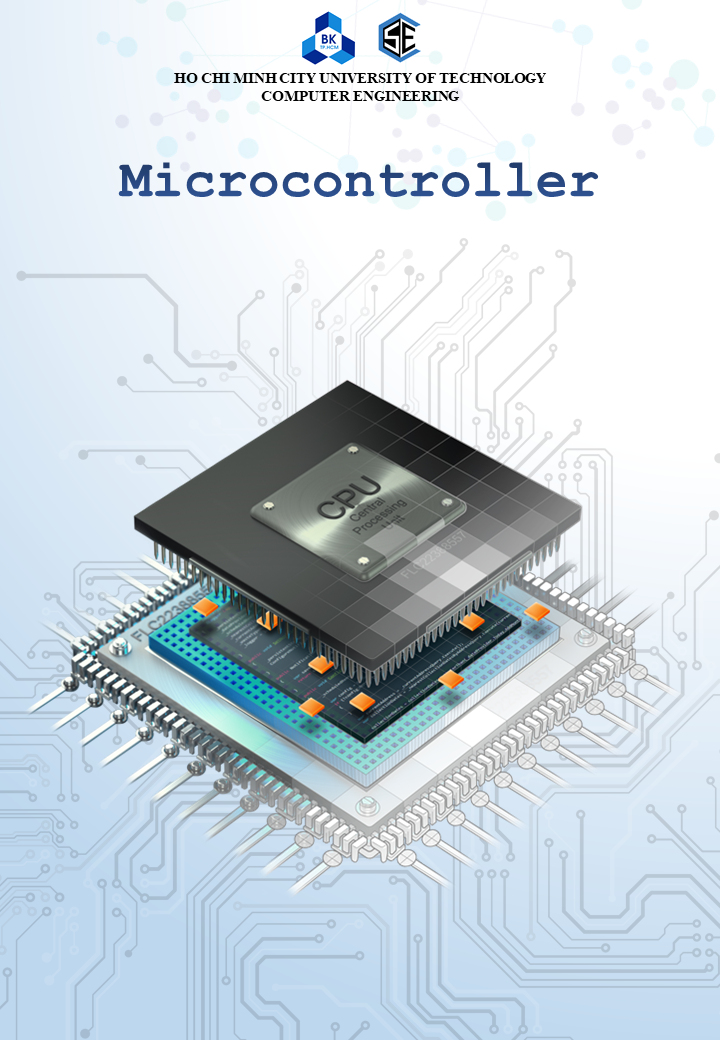
\includegraphics[width=\paperwidth,height=\paperheight]{source/picture/cover.png}}

\begin{textblock*}{22cm}(0cm,27cm)
\begin{center}
    \textbf{Dr. Le Trong Nhan}
\end{center}
\end{textblock*}

\thispagestyle{empty}
\debugline
\newpage

\thispagestyle{empty}
\debugline
\newpage

\thispagestyle{empty}
\begin{center}
\bf{\Large }
\end{center}





\afterpage{\blankpage}

\tableofcontents
\lstset{style=codingstyle}

\chap{LED Animations}

\section{Introduction}
In this manual, the STM32CubeIDE is used as an editor to program the ARM micro-controller. STM32CubeIDE is an advanced C/C++ development platform with peripheral configuration, code generation, code compilation, and debug features for STM32 microcontrollers and microprocessors.\\

\begin{figure}[!htp]
    \centering
    
\includegraphics[width=4in]{source/picture/bai_1/cubeide.jpg}
    \caption{\textit{STM32Cube IDE for STM32 Programming}}
    \label{bai1_cube}
\end{figure}

The most interest of STM32CubeIDE is that after the selection of an empty STM32 MCU or MPU, or preconfigured microcontroller or microprocessor from the selection of a board, the initialization code generated automatically. At any time during the development, the user can return to the initialization and configuration of the peripherals or middleware and regenerate the initialization code with no impact on the user code. This feature can simplify the initialization process and speedup the development application running on STM32 micro-controller. The software can be downloaded from the link bellow:
\begin{center}
    \link{https://ubc.sgp1.digitaloceanspaces.com/BKU\_Softwares/STM32/stm32cubeide\_1.7.0.zip}
\end{center}

Moreover, for a hangout class, the program is firstly simulated on Proteus. Students are also supposed to download and install this software as well:

\begin{center}
    \link{https://ubc.sgp1.digitaloceanspaces.com/BKU\_Softwares/STM32/Proteus\_8.10\_SP0\_Pro.exe}
\end{center}

The rest of this manual consists of:
\begin{itemize}
    \item Create a project on STM32Cube IDE
    \item Create a project on Proteus
    \item Simulate the project on Proteus
\end{itemize}

Finally, students are supposed to finish 10 different projects. 

\newpage
\section{First project on STM32Cube}
\textbf{Step 1: } Launch STM32CubeIDE, from the menu \textbf{File}, select \textbf{New}, then chose \textbf{STM32 Project} 

\begin{figure}[!htp]
    \centering
    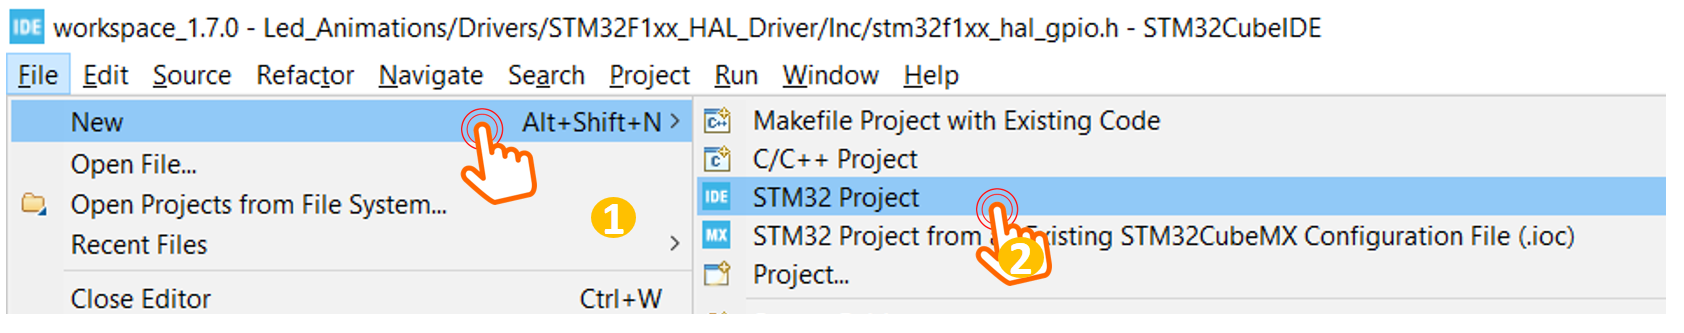
\includegraphics[width=5in]{source/picture/bai_1/stm_01.PNG}
    \caption{\textit{Create a new project on STM32CubeIDE}}
    \label{bai1_stm1}
\end{figure}

The IDE needs to download some packages, which normally takes time in this first time a project is created.\\

\textbf{Step 2: } Select the STM32F103C6 in the following dialog, then click on \textbf{Next}

\begin{figure}[!htp]
    \centering
    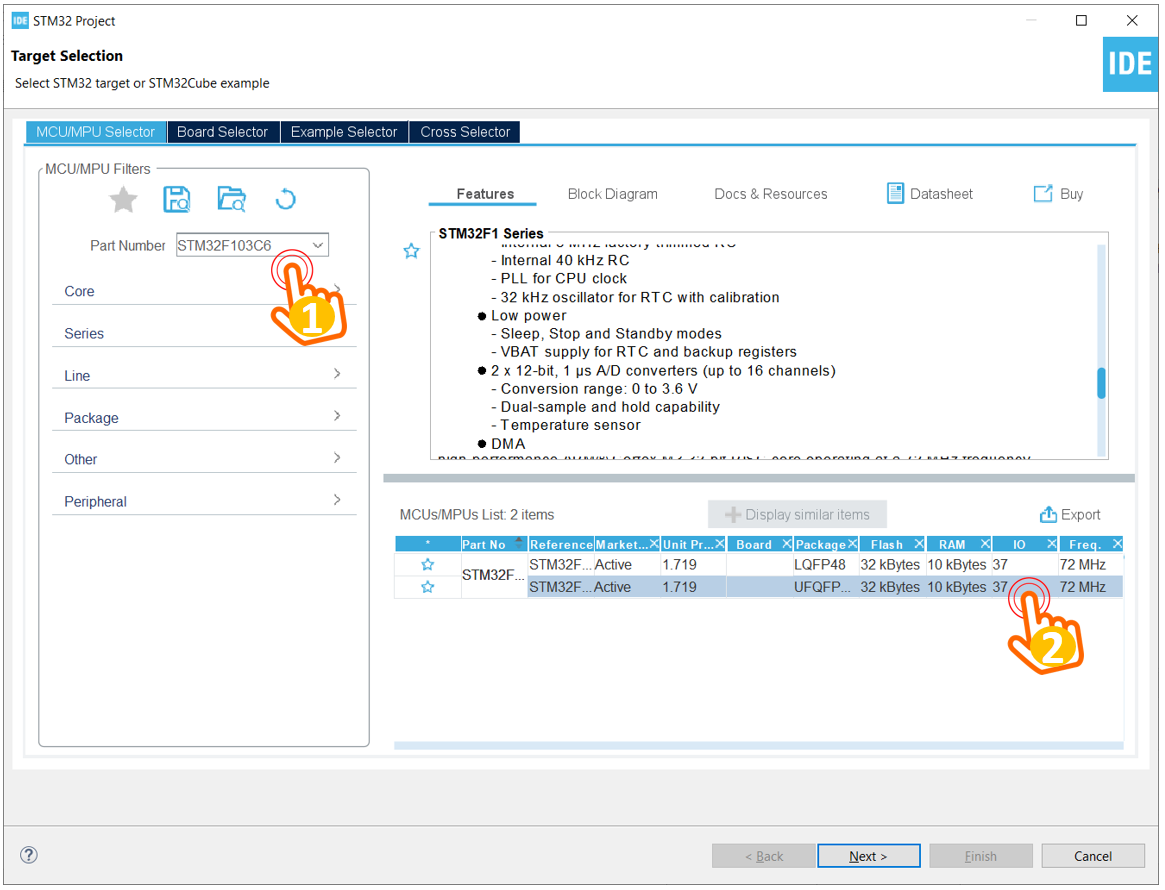
\includegraphics[width=5in]{source/picture/bai_1/stm_02.PNG}
    \caption{\textit{Select the target device}}
    \label{bai1_stm2}
\end{figure}

\textbf{Step 3: } Provide the \textbf{Name} and the \textbf{Location} for the project.

\newpage
\begin{figure}[!htp]
    \centering
    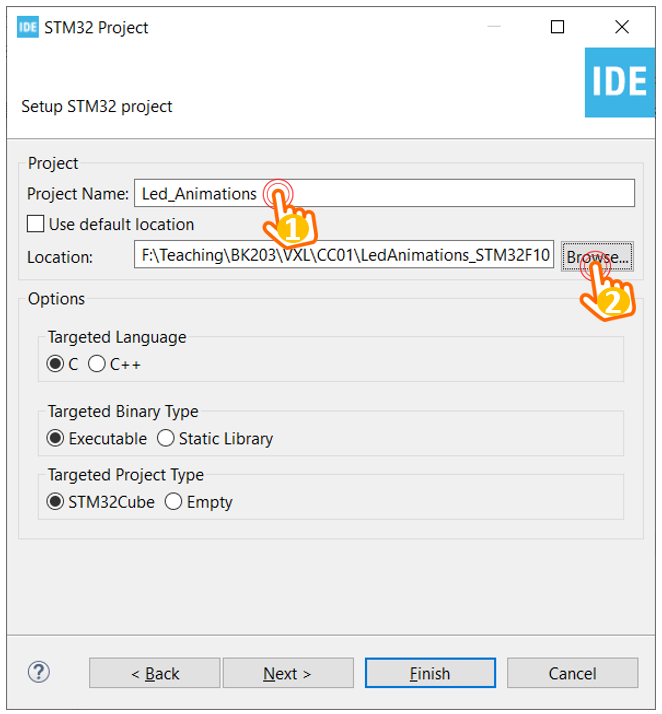
\includegraphics[width=3.5in]{source/picture/bai_1/stm_03.PNG}
    \caption{\textit{Select the target device}}
    \label{bai1_stm3}
\end{figure}

It is important to notice that the \textbf{Targeted Project Type} should be \textbf{STM32Cube}. In the case this option is disable, step 1 must be repeated. The location path should not contain special characters (e.g. the space). Finally, click on the \textbf{Next} button.\\

\textbf{Step 4: } On the last dialog, just keep the default firmware version and click on \textbf{Finish} button.

\begin{figure}[!htp]
    \centering
    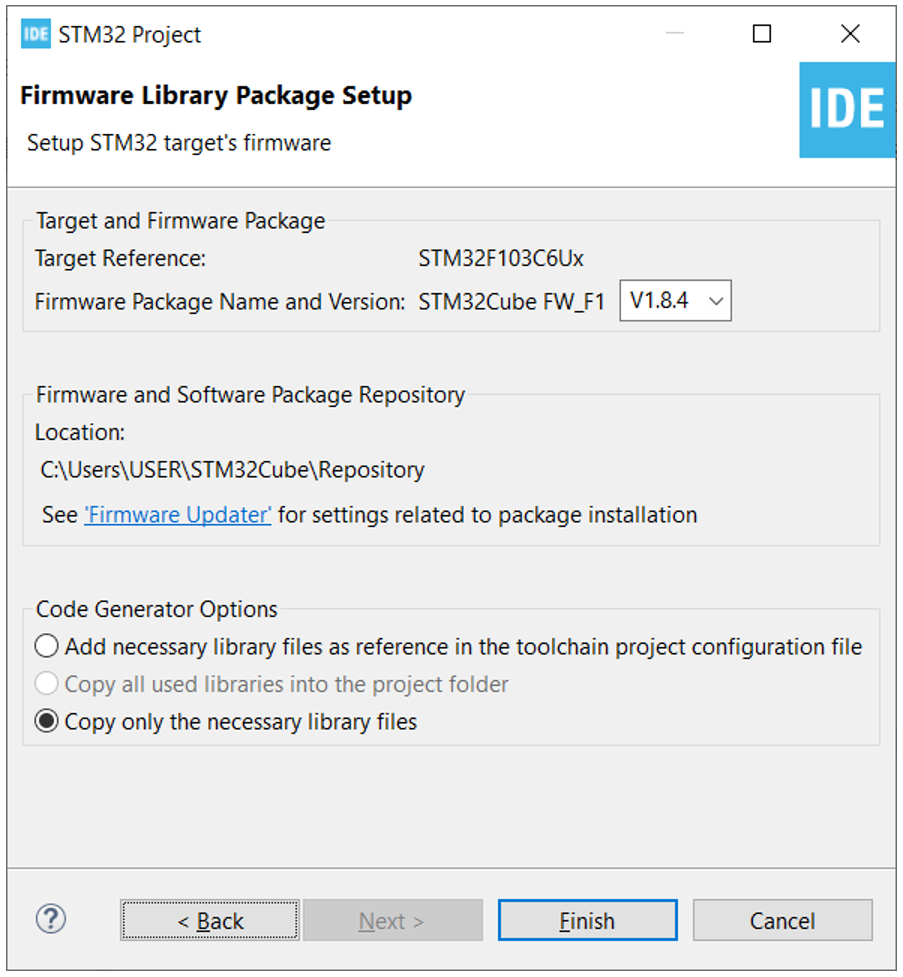
\includegraphics[width=3.5in]{source/picture/bai_1/stm_04.PNG}
    \caption{\textit{Keep default firmware version}}
    \label{bai1_stm4}
\end{figure}

\textbf{Step 5: } The project is created and the wizard for configuration is display. This utility from CubeIDE can simplify the configuration process for an ARM micro-controller like the STM32.

\begin{figure}[!htp]
    \centering
    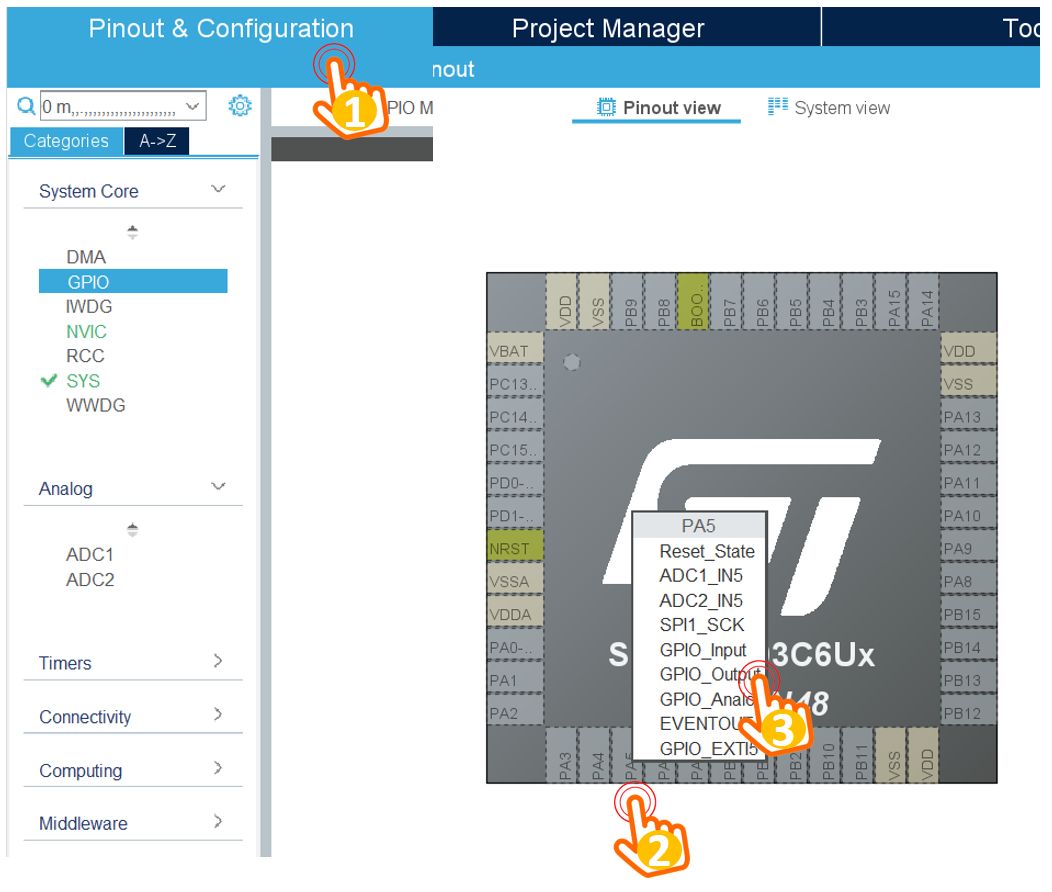
\includegraphics[width=3.5in]{source/picture/bai_1/stm_05.PNG}
    \caption{\textit{Set PA5 to GPIO Output mode}}
    \label{bai1_stm5}
\end{figure}

From the configuration windows, select \textbf{Pin configuration}, select the pin \textbf{PA5} and set to \textbf{GPIO Output} mode, since this pin is connected to an LED in the STM32 development kit.\\

\textbf{Step 6: } Right click on PA5 and select \textbf{Enter user lable}, and provide the name for this pin (e.g. \textbf{LED\_RED}). This step helps programming afterward more memorable.

\begin{figure}[!htp]
    \centering
    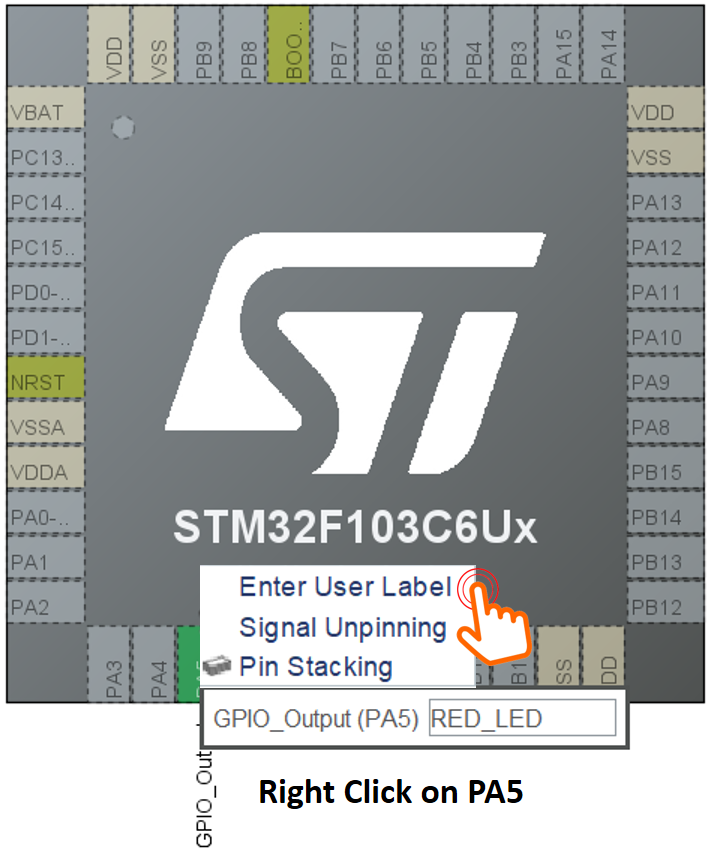
\includegraphics[width=2.5in]{source/picture/bai_1/stm_06.PNG}
    \caption{\textit{Provide a name for PA5}}
    \label{bai1_stm6}
\end{figure}

Finally, save the configuration process by pressing \textbf{Ctrl + S} and confirm this step by clicking on \textbf{OK} button. The code generation is started.\\

\textbf{Step 7: } Implement the first blinky project in the main function as follow:
\begin{lstlisting}[caption=First blinky LED project]
int main(void)
{
  /* USER CODE BEGIN 1 */

  /* USER CODE END 1 */

  /* MCU Configuration--------------------------------------------------------*/

  /* Reset of all peripherals, Initializes the Flash interface and the Systick. */
  HAL_Init();

  /* USER CODE BEGIN Init */

  /* USER CODE END Init */

  /* Configure the system clock */
  SystemClock_Config();

  /* USER CODE BEGIN SysInit */

  /* USER CODE END SysInit */

  /* Initialize all configured peripherals */
  MX_GPIO_Init();
  /* USER CODE BEGIN 2 */

  /* USER CODE END 2 */

  /* Infinite loop */
  /* USER CODE BEGIN WHILE */
 
  while (1)
  {
	  HAL_GPIO_TogglePin(LED_RED_GPIO_Port, LED_RED_Pin);
	  HAL_Delay(1000);
    /* USER CODE END WHILE */

    /* USER CODE BEGIN 3 */
  }
  /* USER CODE END 3 */
}
\end{lstlisting}

Actually, what is added to the main function is line number 34 and 35. Please put your code in a right place, otherwise it can be deleted when the code is generated (e.g. change the configuration of the project). When coding, frequently use the suggestions by pressing \textbf{Ctrl+Space}.

\textbf{Step 7: } Due to the simulation on Proteus, the hex file should be generated from STM32Cube IDE. From menu \textbf{Project}, select \textbf{Properties} to open the dialog bellow:

\begin{figure}[!htp]
    \centering
    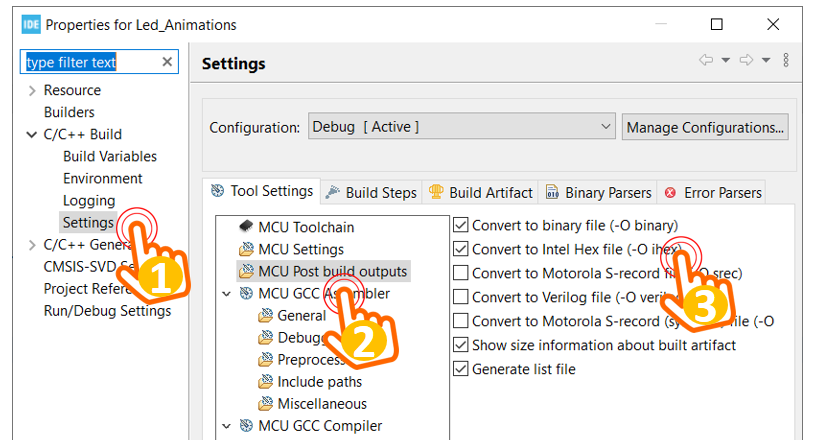
\includegraphics[width=5in]{source/picture/bai_1/stm_07.PNG}
    \caption{\textit{Config for hex file output}}
    \label{bai1_pic5}
\end{figure}

Navigate to \textbf{C/C++ Build}, select \textbf{Settings, MCU Post build outputs}, and check to the \textbf{Intel Hex file}. \\

\textbf{Step 8: } Build the project by clicking on menu \textbf{Project} and select \textbf{Build Project}. Please check on the output console of the IDE to be sure that the hex file is generated, as follow:

\begin{figure}[!htp]
    \centering
    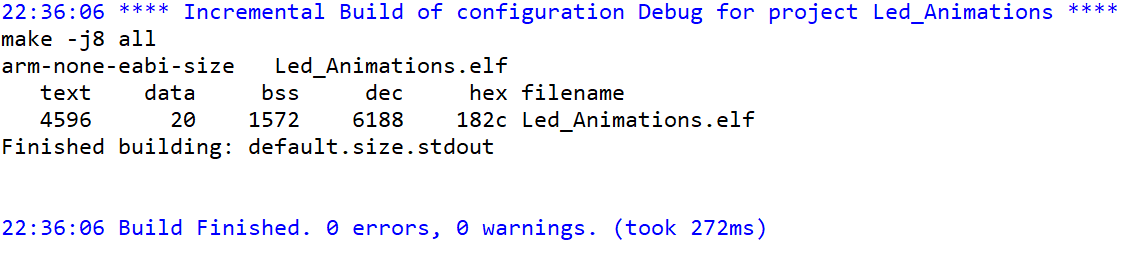
\includegraphics[width=5in]{source/picture/bai_1/stm_08.PNG}
    \caption{\textit{Compile the project and generate Hex file}}
    \label{bai1_pic8}
\end{figure}

The hex file is located under the \textbf{Debug} folder of your project, which is used for the simulation in Proteus afterward. In the case a development kit is connected to your PC, from menu \textbf{Run}, select \textbf{Run} to download the program to the hardware platform. \\

In the case there are multiple project in a work-space, double click on the project name to activate this project. Whenever a project is built, check the output files to make sure that you are working in a right project.


\newpage
\section{Simulation on Proteus}
For an online training, a simulation on Proteus can be used. The details to create an STM32 project on Proteus are described bellow.\\

\textbf{Step 1: } Launch Proteus (\textbf{with administration access}) and from menu \textbf{File}, select \textbf{New Project}.\\

\begin{figure}[!htp]
    \centering
    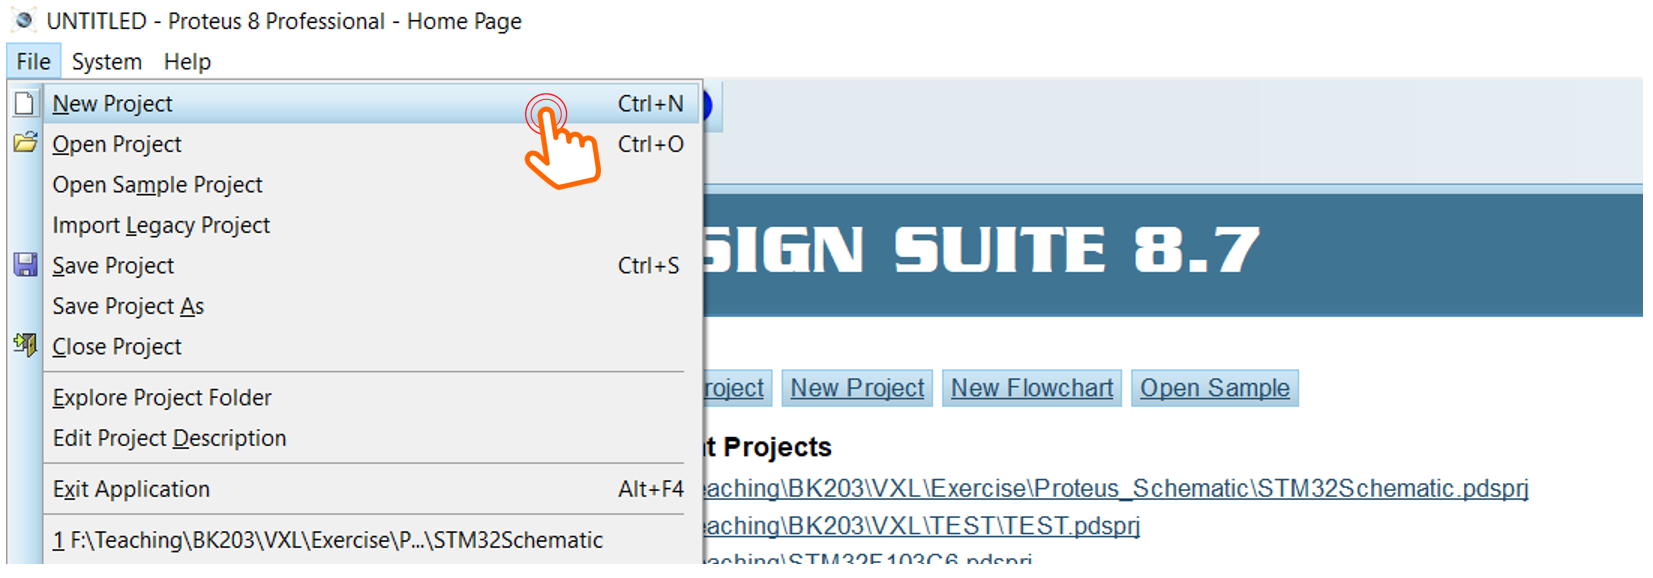
\includegraphics[width=5in]{source/picture/bai_1/pic5.PNG}
    \caption{\textit{Create a new project on Proteus}}
    \label{bai1_pic5}
\end{figure}


\textbf{Step 2: } Provide the name and the location of the project, then click on \textbf{Next} button.\\

\begin{figure}[!htp]
    \centering
    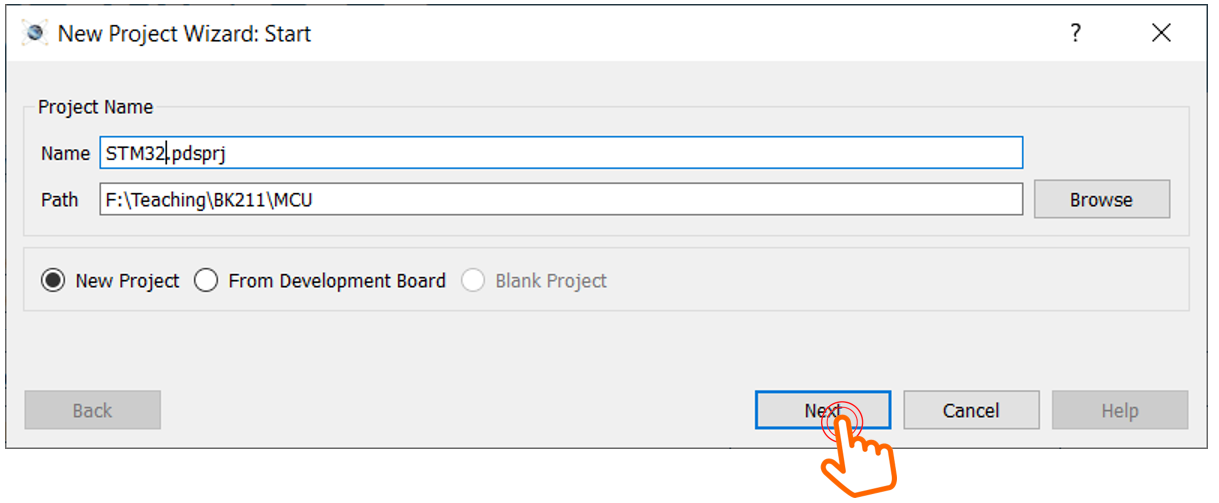
\includegraphics[width=4in]{source/picture/bai_1/pic6.PNG}
    \caption{\textit{Provide project name and location}}
    \label{bai1_pic6}
\end{figure}

\textbf{Step 3: } For following dialog, just click on \textbf{Next} button as just a schematic is required for the lab.

\begin{figure}[!htp]
    \centering
    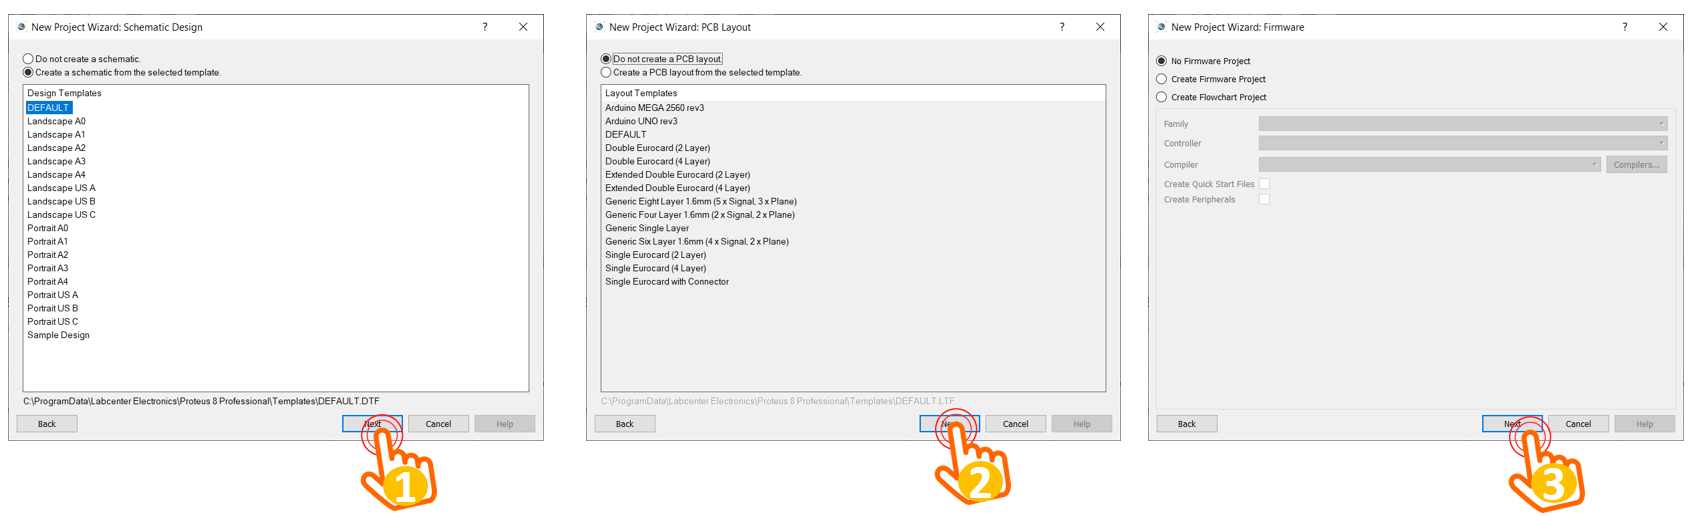
\includegraphics[width=5.5in]{source/picture/bai_1/pic7.PNG}
    \caption{\textit{Keep the default options by clicking on Next}}
    \label{bai1_pic7}
\end{figure}
\newpage
\textbf{Step 4: } Finally, click on \textbf{Finish} button to close the project wizard. \\

\begin{figure}[!htp]
    \centering
    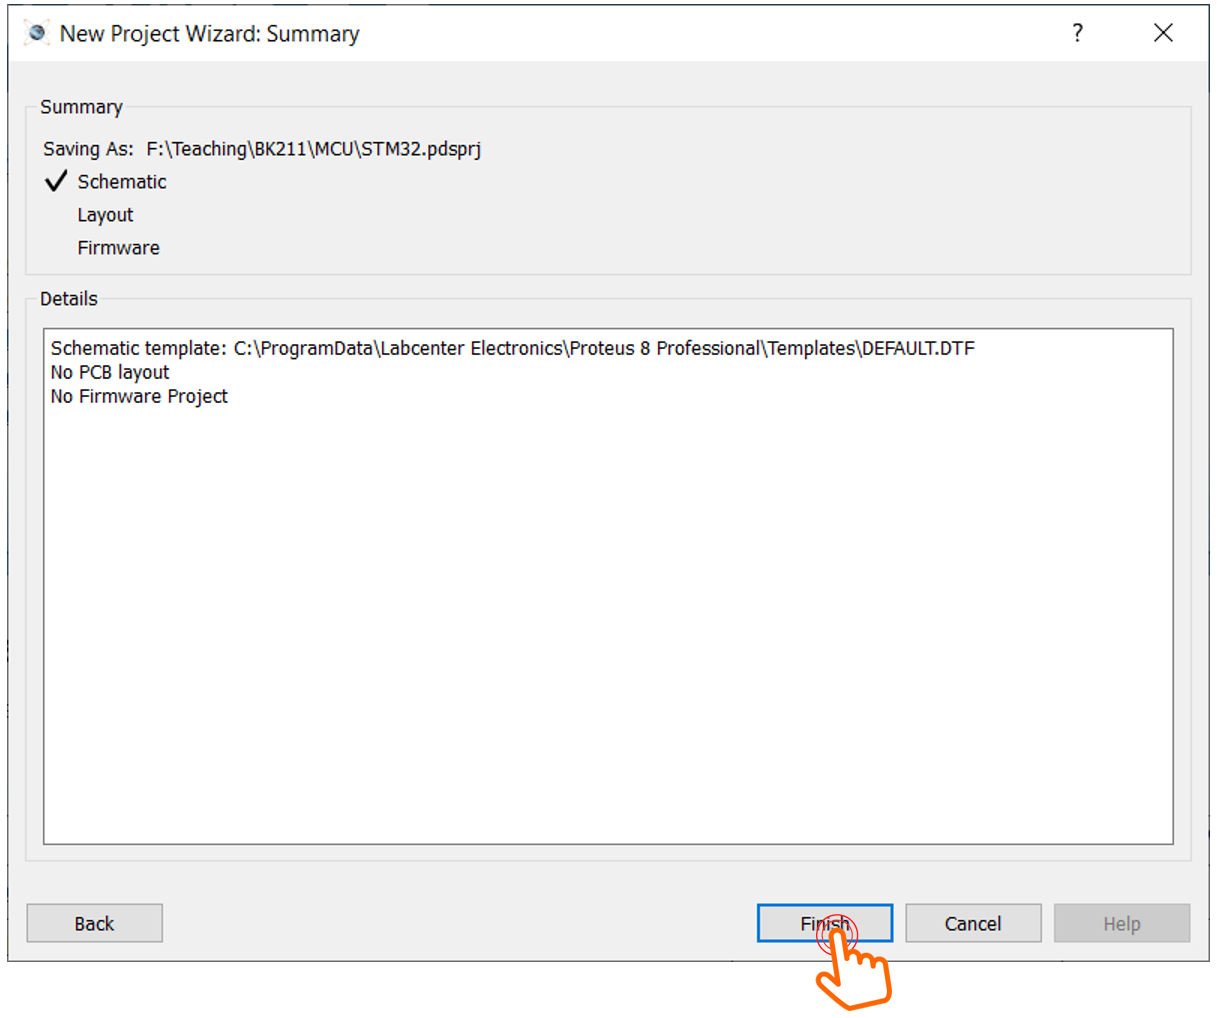
\includegraphics[width=4in]{source/picture/bai_1/pic8.PNG}
    \caption{\textit{Finish the project wizard}}
    \label{bai1_pic8}
\end{figure}

\textbf{Step 5: } On the main page of the project, right click to select \textbf{Place, Components, From Libraries}, as follows:
\begin{figure}[!htp]
    \centering
    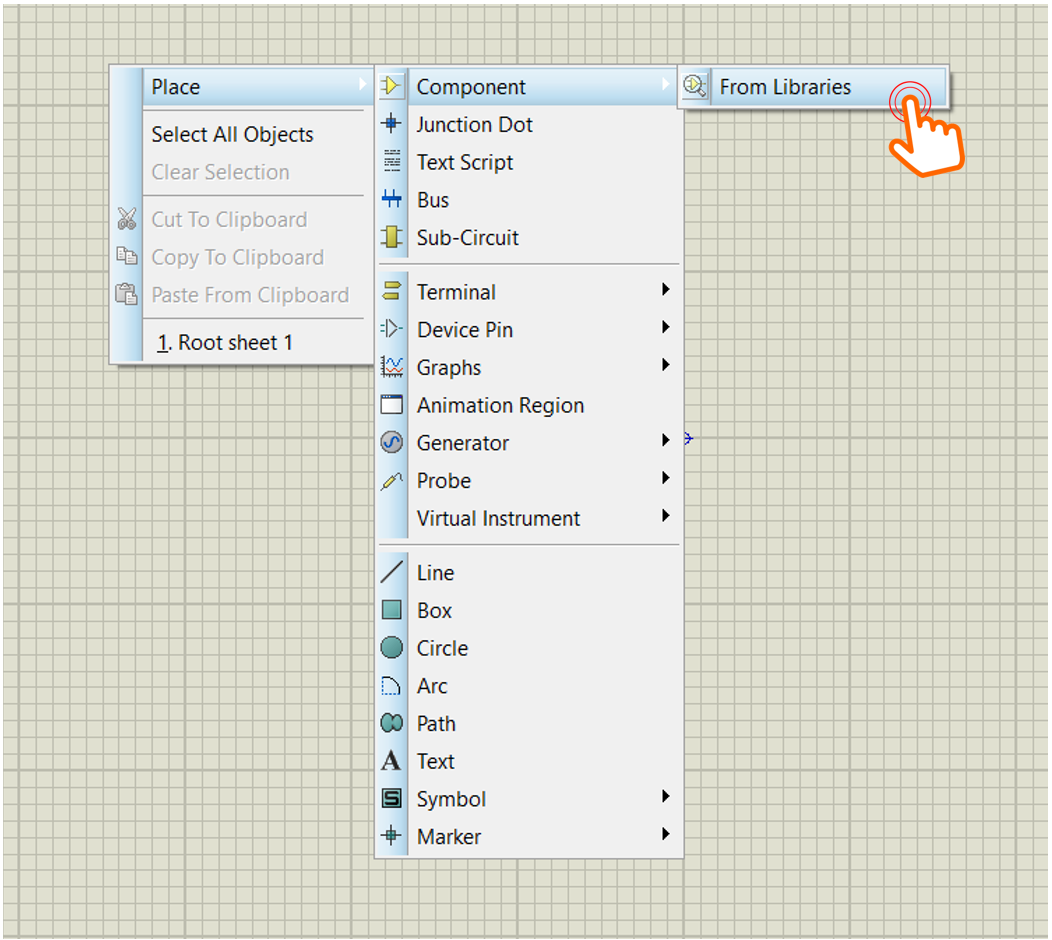
\includegraphics[width=4in]{source/picture/bai_1/pic9.PNG}
    \caption{\textit{Select a component from the library}}
    \label{bai1_pic9}
\end{figure}

\textbf{If there is an error with no library found, please restart the Proteus software with Run as administrator option.\\}

\textbf{Step 6: } From the list of components in the library, select STM32F103C6, as follows:

\begin{figure}[!htp]
    \centering
    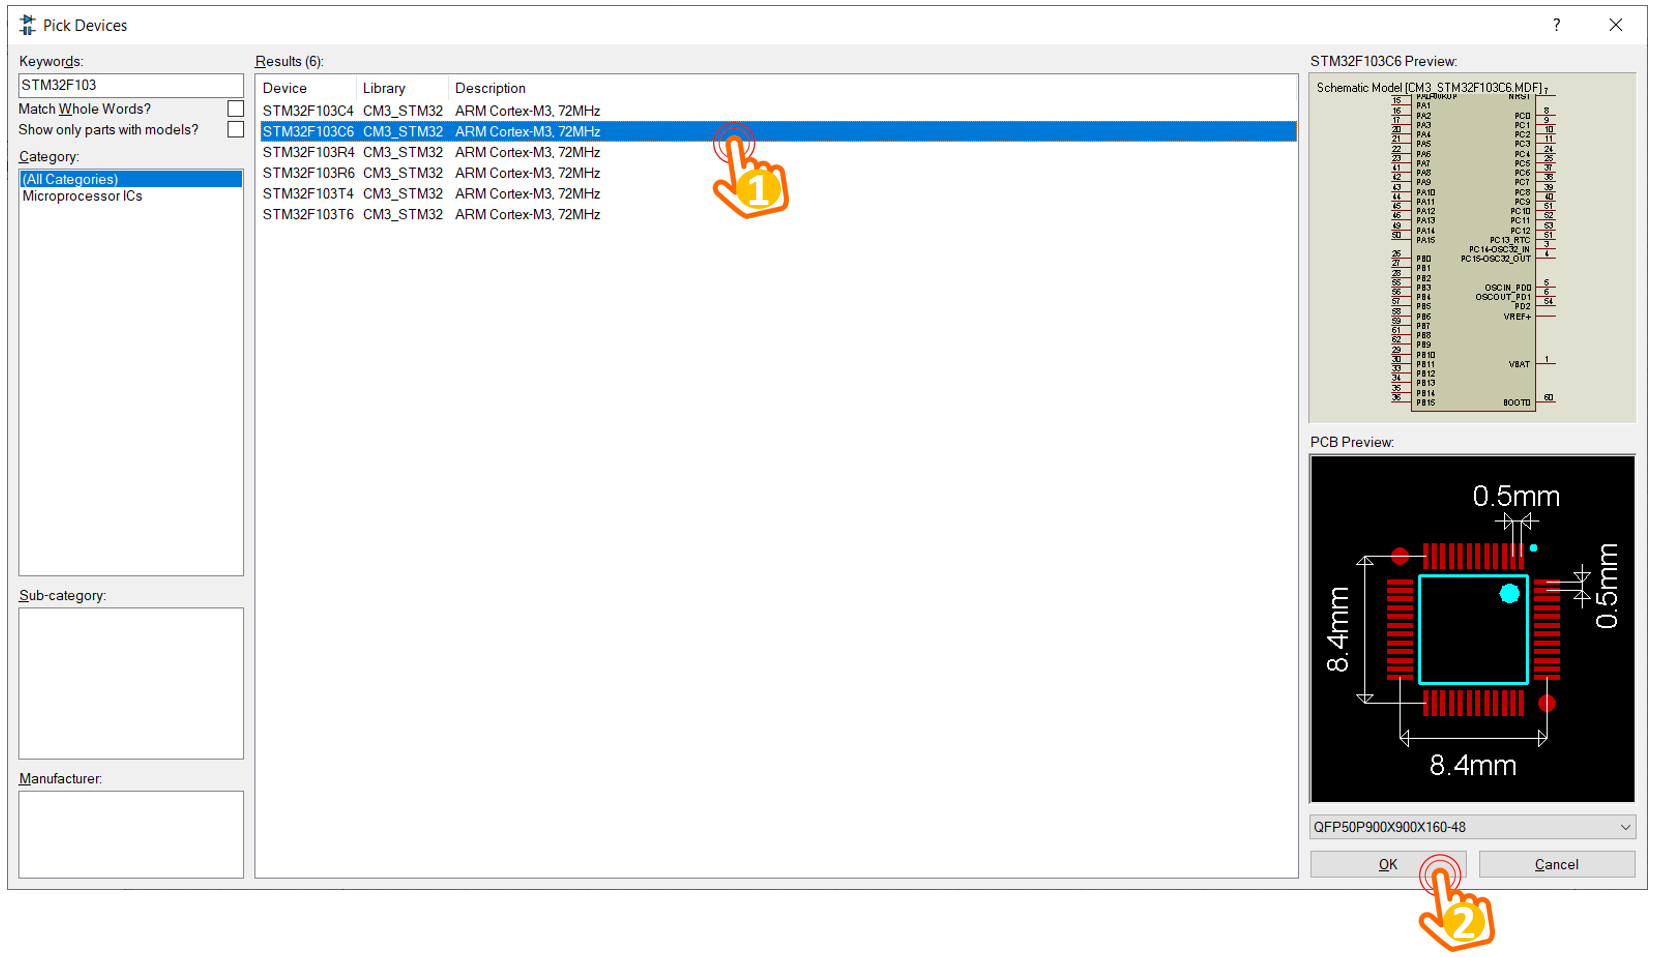
\includegraphics[width=5.5in]{source/picture/bai_1/pic10.PNG}
    \caption{\textit{Select STM32F103C6}}
    \label{bai1_pic10}
\end{figure}

Repeat step 5 and 6 to select an LED, named \textbf{LED-RED} in Proteus. Finally, these components are appeared on the DEVICES windows, which is on left hand side as follows:
\begin{figure}[!htp]
    \centering
    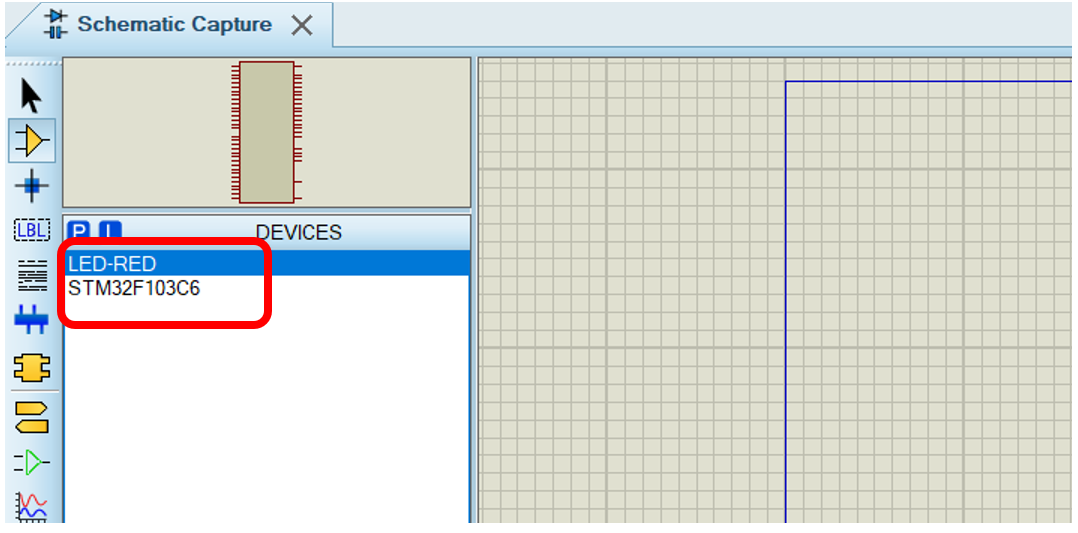
\includegraphics[width=4in]{source/picture/bai_1/pic11.PNG}
    \caption{\textit{STM32 and an LED in the project}}
    \label{bai1_pic9}
\end{figure}

\textbf{Step 7: } Place the components to the project: right click on the main page, select on \textbf{Place, Component}, and select device added in Step 6. To add the Power and the Ground,  right click on the main page, select on \textbf{Place, Terminal}. The result in this step is expected as follows:
\newpage
\begin{figure}[!htp]
    \centering
    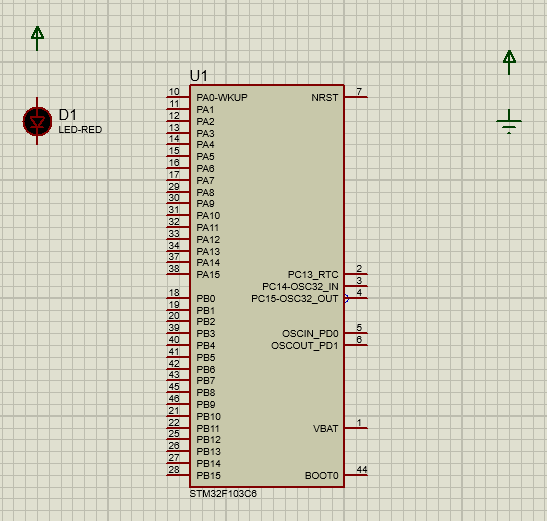
\includegraphics[width=4in]{source/picture/bai_1/pic14.PNG}
    \caption{\textit{Place components to the project}}
    \label{bai1_pic14}
\end{figure}

\textbf{Step 8: } Start wiring the circuit. The negative pin of the LED is connected to PA5 while its positive pin is connected to the power supply. For the power and the ground on the right, just make a short wire, which will labeled in the next step.

\begin{figure}[!htp]
    \centering
    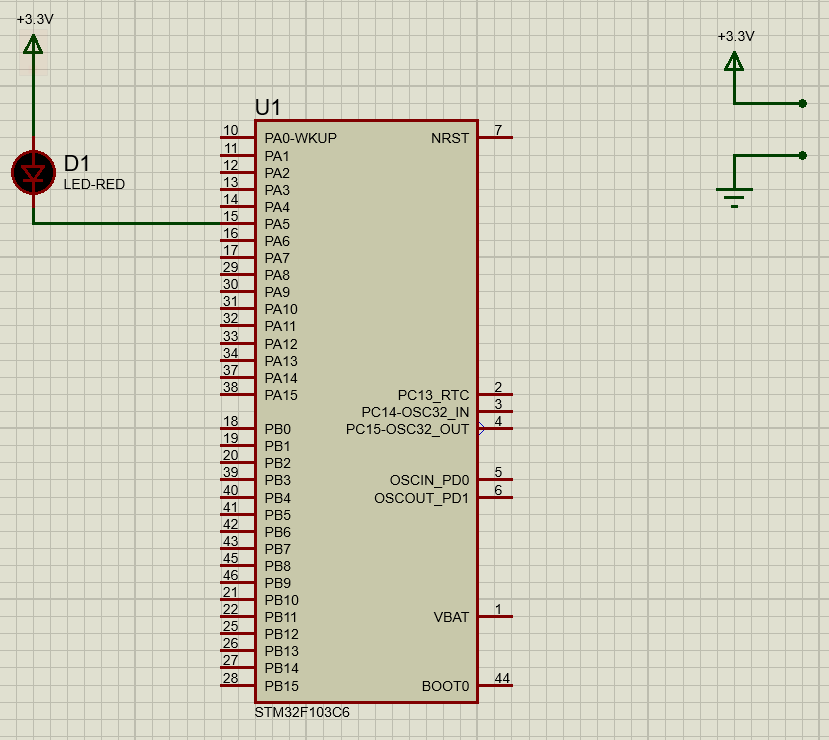
\includegraphics[width=4in]{source/picture/bai_1/pic15.PNG}
    \caption{\textit{Connect components and set the power to 3.3V}}
    \label{bai1_pic15}
\end{figure}

In this step, also double click on the power supply in order to provide the String property to \textbf{+3.3V}.

\textbf{Step 8: } Right click on the wire of the power supply and the ground, and select \textbf{Place wire Label}

\begin{figure}[!htp]
    \centering
    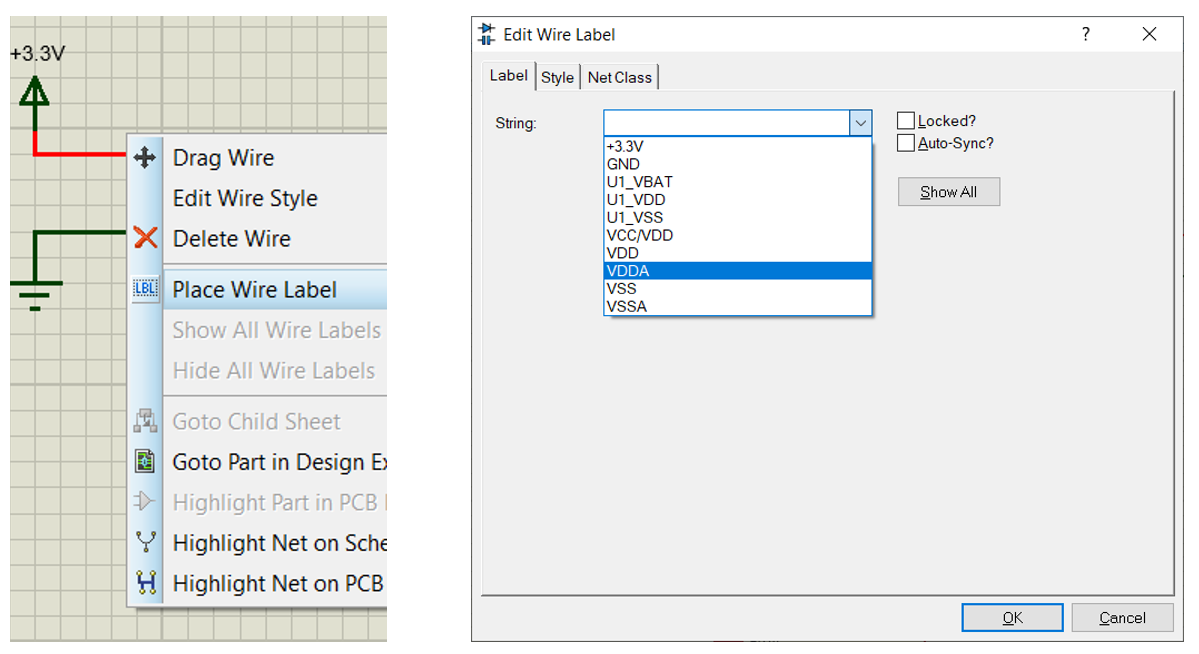
\includegraphics[width=4in]{source/picture/bai_1/pic16.PNG}
    \caption{\textit{Place label for Power and Ground}}
    \label{bai1_pic16}
\end{figure}

This step is required as VDDA and VSSA of the STM32 must be connected to provide the reference voltage. Therefore, VDDA is connected to 3.3V, while the VSSA is connected to the Ground. Finally, the image of our schematic is shown bellow:

\begin{figure}[!htp]
    \centering
    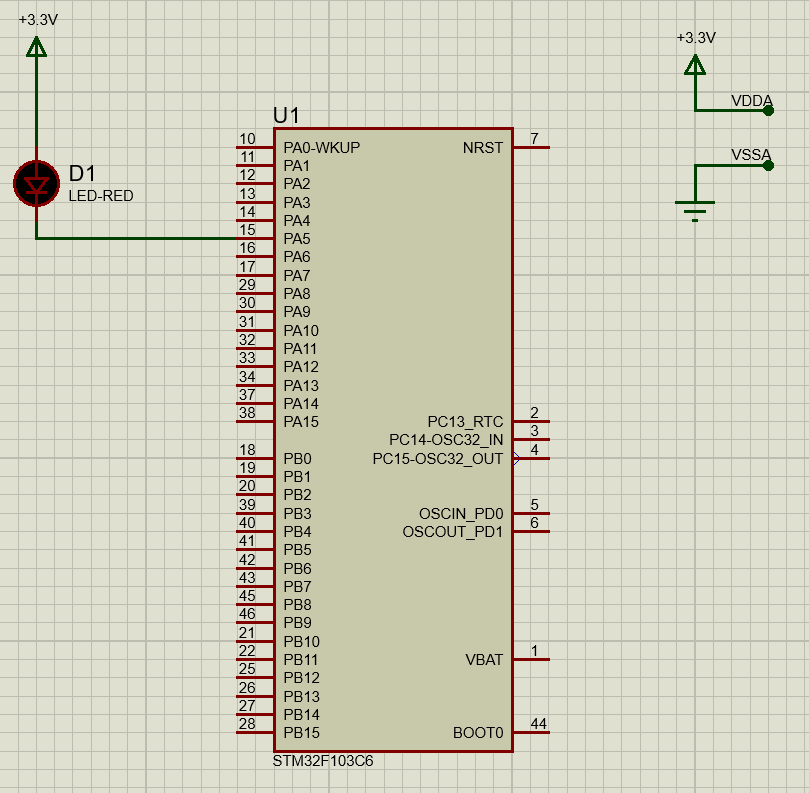
\includegraphics[width=4in]{source/picture/bai_1/pic17.PNG}
    \caption{\textit{Finalize the schematic}}
    \label{bai1_pic17}
\end{figure}
\newpage
\textbf{Step 9: } Double click on the STM32, and set the \textbf{Program File} to the Hex file, which is generated from Cube IDE, as following:

\begin{figure}[!htp]
    \centering
    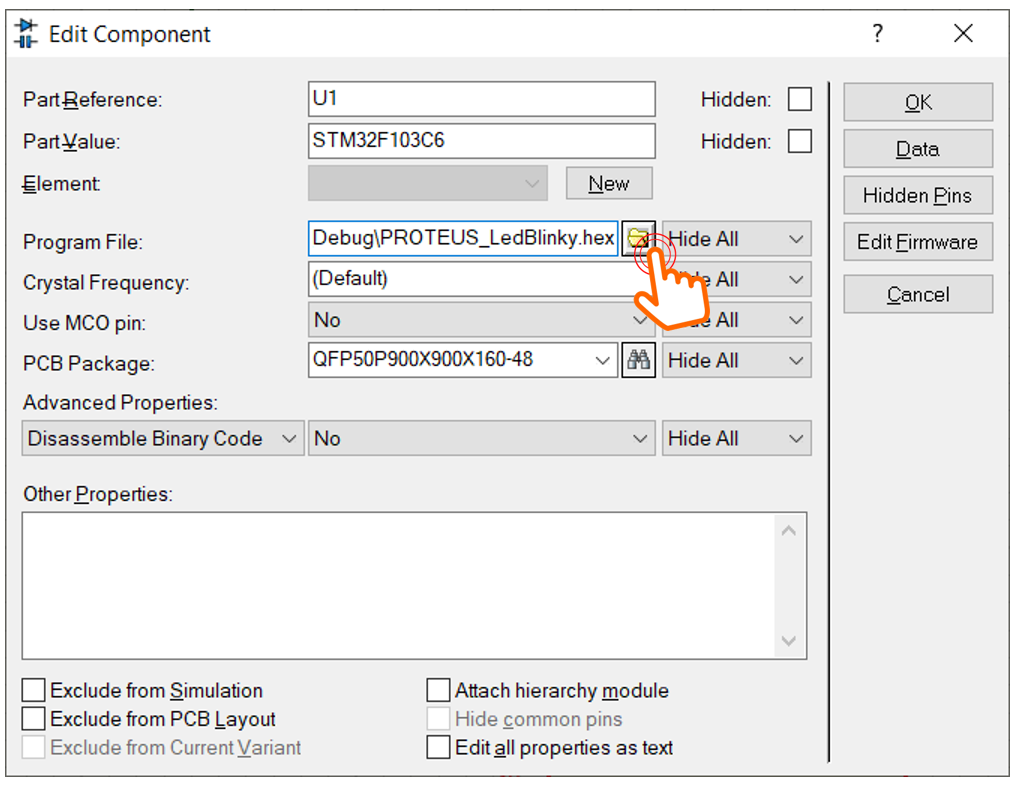
\includegraphics[width=4in]{source/picture/bai_1/pic18.PNG}
    \caption{\textit{Set the program of the STM32 to the hex file from Cube IDE}}
    \label{bai1_pic18}
\end{figure}

From now, the simulation is ready to start by clicking on the menu \textbf{Debug}, and select on \textbf{Run simulation}. To stop the simulation, click on \textbf{Debug} and select \textbf{Stop VMS Debugging}. Moreover, there are some quick access bottom on the left corner of the Proteus to start or stop the simulation, as shown following:\\
\begin{figure}[!htp]
    \centering
    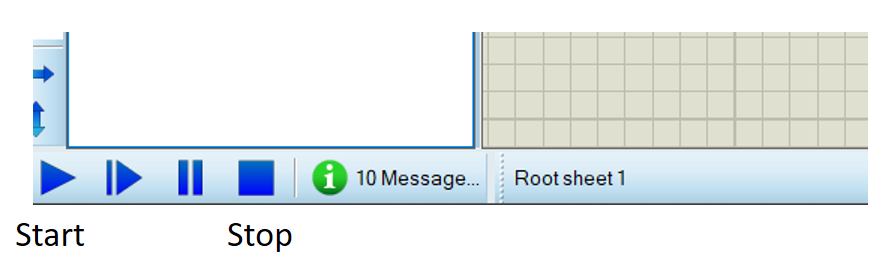
\includegraphics[width=4in]{source/picture/bai_1/pic18a.PNG}
    \caption{\textit{Quick access buttons to start and stop the simulation}}
    \label{bai1_pic18}
\end{figure}

If everything is success, students can see the LED is blinking every second. Please stop the simulation before updating the project, either in Proteus or STM32Cube IDE. However, the step 9 (set the program file for STM32 in Proteus) is required to do once. Beside the toggle instruction, student can set or reset a pin as following:

\begin{lstlisting}[caption=An example for LED blinky]
while (1){
  HAL_GPIO_WritePin(LED_RED_GPIO_Port, LED_RED_Pin, GPIO_PIN_SET);
  HAL_Delay(1000);
  HAL_GPIO_WritePin(LED_RED_GPIO_Port, LED_RED_Pin, GPIO_PIN_RESET);
  HAL_Delay(1000);
}
\end{lstlisting}
\newpage
\section{Exercise and Report}
\subsection{Exercise 1}
From the simulation on Proteus, one more LED is connected to pin \textbf{PA6} of the STM32 (negative pin of the LED is connected to PA6). The component suggested in this exercise is \textbf{LED-YELLOW}, which can be found from the device list.\\



In this exercise, the status of two LEDs are switched every 2 seconds, as demonstrated in the figure bellow.

\begin{figure}[!htp]
    \centering
    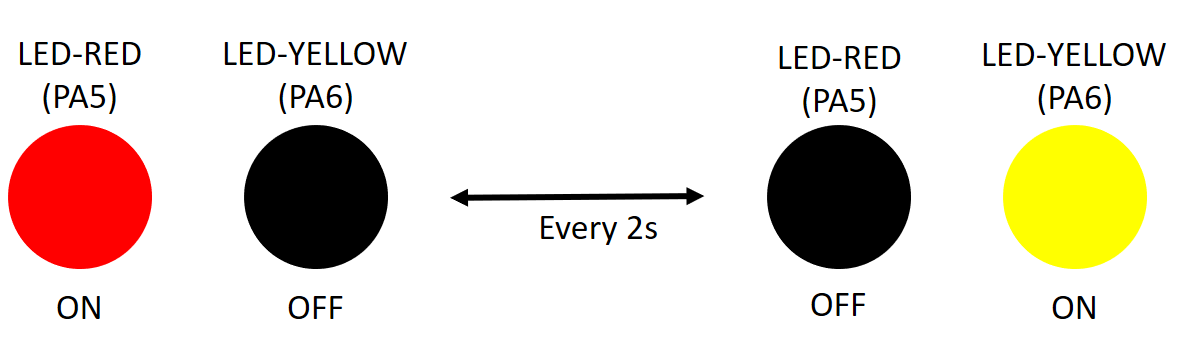
\includegraphics[width=5in]{source/picture/bai_1/pic1.PNG}
    \caption{\textit{State transitions for 2 LEDs}}
    \label{bai1_pic1}
\end{figure}

\textbf{Report 1: }Depict the schematic from Proteus simulation in this report. The caption of the figure is a downloadable link to the Proteus project file (e.g. a github link).
\begin{figure}[!htp]
    \centering
    \includegraphics[width=5in]{source/Image/bai1.png}
\end{figure}

\textbf{Report 2: } Present the source code in the infinite loop while of your project. If a user-defined functions is used, it is required to present in this part. A brief description can be added for this function (e.g. using comments). A template to present your source code is presented bellow.

\begin{lstlisting}[caption=An example for your source code]
  int counter = 4;
  int reset_counter = 4;
  int flag = 0; // red = 0 yellow = 1
  while (1)
  {
	  if (counter <= 0) {
		  counter = reset_counter;
	  }
	  if (counter > 2) {
		  flag = 0;
	  } else {
		  flag = 1;
	  }
	  if (flag == 0) {
		  HAL_GPIO_WritePin(GPIOA, GPIO_PIN_5, RESET);
		  HAL_GPIO_WritePin(GPIOA, GPIO_PIN_6, SET);
	  } else if (flag == 1) {
		  HAL_GPIO_WritePin(GPIOA, GPIO_PIN_5, SET);
		  HAL_GPIO_WritePin(GPIOA, GPIO_PIN_6, RESET);
	  }
	  counter--;
	  HAL_Delay(1000);
    /* USER CODE END WHILE */

    /* USER CODE BEGIN 3 */
  }
\end{lstlisting}

\subsection{Exercise 2}
Extend the first exercise to simulate the behavior of a traffic light. A third LED, named \textbf{LED-GREEN} is added to the system, which is connected to \textbf{PA7}. A cycle in this traffic light is 5 seconds for the RED, 2 seconds for the YELLOW and 3 seconds for the GREEN. The LED-GREEN is also controlled by its negative pin.\\

Similarly, the report in this exercise includes the schematic of your circuit and a your source code in the while loop.

\textbf{Report 1: } Present the schematic.\\

\begin{figure}[!htp]
    \centering
    \includegraphics[width=5in]{source/Image/bai2.png}
\end{figure}

\textbf{Report 2: } Present the source code in while.\\

\begin{lstlisting}
  int counter = 10;
  int reset_counter = 10;
  int flag = 0; // red = 0 yellow = 1 green = 2
  while (1)
  {
	  if (counter <= 0) {
		  counter = reset_counter;
	  }
	  if (counter > 5) {
		  flag = 0;
	  } else if (counter > 3) {
		  flag = 1;
	  } else {
		  flag = 2;
	  }
	  if (flag == 0) {
		  HAL_GPIO_WritePin(GPIOA, GPIO_PIN_5, RESET);
		  HAL_GPIO_WritePin(GPIOA, GPIO_PIN_6, SET);
		  HAL_GPIO_WritePin(GPIOA, GPIO_PIN_7, SET);
	  } else if (flag == 1) {
		  HAL_GPIO_WritePin(GPIOA, GPIO_PIN_5, SET);
		  HAL_GPIO_WritePin(GPIOA, GPIO_PIN_6, RESET);
		  HAL_GPIO_WritePin(GPIOA, GPIO_PIN_7, SET);
	  } else if (flag == 2) {
		  HAL_GPIO_WritePin(GPIOA, GPIO_PIN_5, SET);
		  HAL_GPIO_WritePin(GPIOA, GPIO_PIN_6, SET);
		  HAL_GPIO_WritePin(GPIOA, GPIO_PIN_7, RESET);
	  }
	  counter--;
	  HAL_Delay(1000);
    /* USER CODE END WHILE */

    /* USER CODE BEGIN 3 */
  }
\end{lstlisting}

\subsection{Exercise 3}
Extend to the 4-way traffic light. Arrange 12 LEDs in a nice shape to simulate the behaviors of a traffic light. A reference design can be found in the figure bellow.

\begin{figure}[!htp]
    \centering
    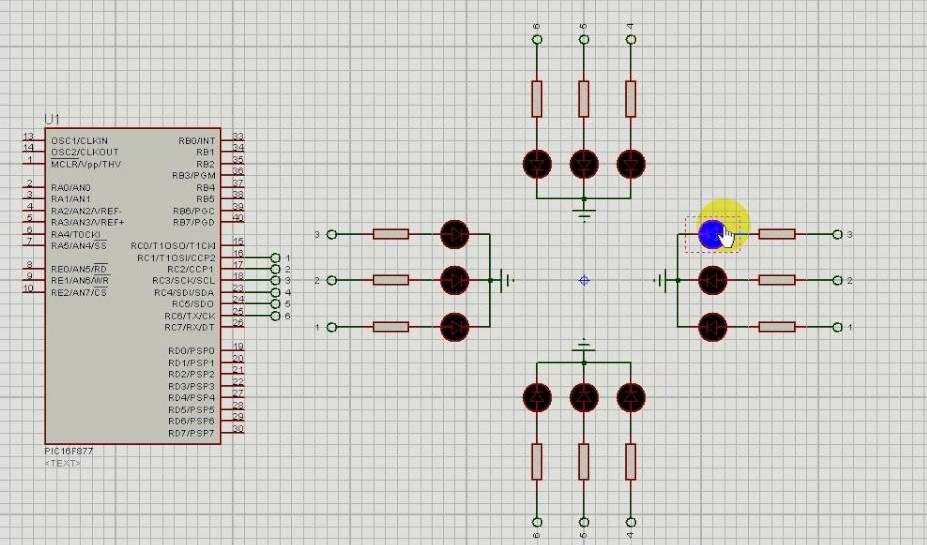
\includegraphics[width=5in]{source/picture/bai_1/pic2.jpg}
    \caption{\textit{Reference design for a 4 way traffic light}}
    \label{bai1_pic2}
\end{figure}

\subsection{Exercise 4}
Add \textbf{only one 7 led segment} to the schematic in Exercise 3. This component can be found in Proteus by the keyword \textbf{7SEG-COM-ANODE}. For this device, the common pin should be connected to the power supply and other pins are supposed to connected to PB0 to PB6. Therefore, to turn-on a segment in this 7SEG, the STM32 pin should be in logic 0 (0V).\\

Implement a function named \textbf{display7SEG(int num)}. The input for this function is from 0 to 9 and the outputs are listed as following:

\begin{figure}[!htp]
    \centering
    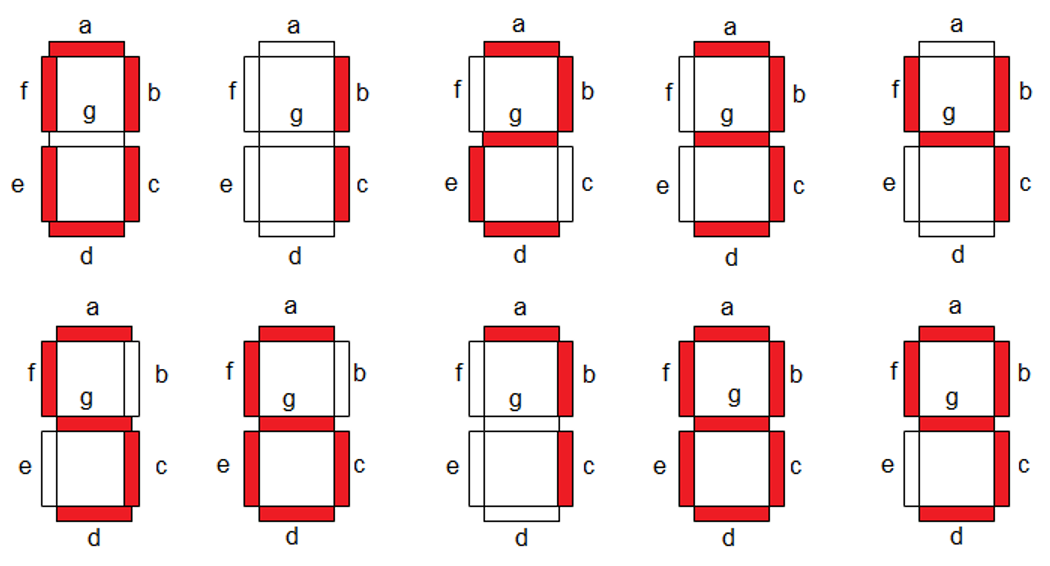
\includegraphics[width=4in]{source/picture/bai_1/pic3.PNG}
    \caption{\textit{Display a number on  7 segment LED}}
    \label{bai1_pic3}
\end{figure}

\newpage
This function is invoked in the while loop for testing as following:
\begin{lstlisting}[caption=An example for your source code]
int counter = 0;
while (1){
    if(counter >= 10) counter = 0;    
    display7SEG(counter++);
    HAL_Delay(1000);

}
\end{lstlisting}

\textbf{Report 1: } Present the schematic.\\

\begin{figure}[!htp]
    \centering
    \includegraphics[width=5in]{source/Image/bai4.png}
\end{figure}

\textbf{Report 2: } Present the source code for display7SEG function.
\begin{lstlisting}
void display7SEG(int num) {
	switch (num) {
		case 0:
			GPIOB->ODR = 0x0040; // 0100 0000
			break;
		case 1:
			GPIOB->ODR = 0x0079; // 0111 1001
			break;
		case 2:
			GPIOB->ODR = 0x0024; // 0010 0100
			break;
		case 3:
			GPIOB->ODR = 0x0030; // 0011 0000
			break;
		case 4:
			GPIOB->ODR = 0x0019; // 0001 1001
			break;
		case 5:
			GPIOB->ODR = 0x0012; // 0001 0010
			break;
		case 6:
			GPIOB->ODR = 0x0002; // 0000 0010
			break;
		case 7:
			GPIOB->ODR = 0x0078; // 0111 1000
			break;
		case 8:
			GPIOB->ODR = 0x0000; // 0000 0000
			break;
		case 9:
			GPIOB->ODR = 0x0010; // 0001 0000
			break;
		default:
			break;
	}
}
\end{lstlisting}

\subsection{Exercise 5}
Integrate the 7SEG-LED to the 4 way traffic light. In this case, the 7SEG-LED is used to display countdown value.\\

In this exercise, only source code is required to present. The function display7SEG in previous exercise can be re-used.
\begin{figure}[!htp]
    \centering
    \includegraphics[width=5in]{source/Image/bai5.png}
\end{figure}
\begin{lstlisting}
unsigned int buffer = 0x0000;
void display7SEG_One(int num) {
	buffer = buffer & 0xFF00;
	switch (num) {
		case 0:
			buffer += 0x0040; // 0100 0000
			break;
		case 1:
			buffer += 0x0079; // 0111 1001
			break;
		case 2:
			buffer += 0x0024; // 0010 0100
			break;
		case 3:
			buffer += 0x0030; // 0011 0000
			break;
		case 4:
			buffer += 0x0019; // 0001 1001
			break;
		case 5:
			buffer += 0x0012; // 0001 0010
			break;
		case 6:
			buffer += 0x0002; // 0000 0010
			break;
		case 7:
			buffer += 0x0078; // 0111 1000
			break;
		case 8:
			buffer += 0x0000; // 0000 0000
			break;
		case 9:
			buffer += 0x0010; // 0001 0000
			break;
		default:
			break;
	}
	GPIOB->ODR = buffer;
}
void display7SEG_Two(int num) {
	buffer = buffer & 0x00FF;
	switch (num) {
		case 0:
			buffer += 0x4000; // 0100 0000
			break;
		case 1:
			buffer += 0x7900; // 0111 1001
			break;
		case 2:
			buffer += 0x2400; // 0010 0100
			break;
		case 3:
			buffer += 0x3000; // 0011 0000
			break;
		case 4:
			buffer += 0x1900; // 0001 1001
			break;
		case 5:
			buffer += 0x1200; // 0001 0010
			break;
		case 6:
			buffer += 0x0200; // 0000 0010
			break;
		case 7:
			buffer += 0x7800; // 0111 1000
			break;
		case 8:
			buffer += 0x0000; // 0000 0000
			break;
		case 9:
			buffer += 0x1000; // 0001 0000
			break;
		default:
			break;
	}
	GPIOB->ODR = buffer;
}
  int counter = 10;
  int reset_counter = 10;
  int time_7SEG1 = 3, time_7SEG2 = 5;
  int flag1, flag2; // red = 0 yellow = 1 green = 2
  while (1)
  {
	  if (counter == 7) {
		  time_7SEG1 = 2;
	  } else if (counter == 5) {
		  time_7SEG1 = 5;
	  } else if (counter == 0) {
		  time_7SEG1 = 3;
	  }
	  if (counter == 5) {
		  time_7SEG2 = 3;
	  } else if (counter == 2) {
		  time_7SEG2 = 2;
	  } else if (counter == 0) {
		  time_7SEG2 = 5;
	  }
	  if (counter <= 0) {
		  counter = reset_counter;
	  }
	  if (counter > 5) {
		  flag1 = 0;
	  } else if (counter > 2) {
		  flag1 = 2;
	  } else {
		  flag1 = 1;
	  }
	  if (counter > 7) {
		  flag2 = 2;
	  } else if (counter > 5) {
		  flag2 = 1;
	  } else {
		  flag2 = 0;
	  }
	  if (flag1 == 0) {
		  HAL_GPIO_WritePin(GPIOA, GPIO_PIN_1, SET);
		  HAL_GPIO_WritePin(GPIOA, GPIO_PIN_2, RESET);
		  HAL_GPIO_WritePin(GPIOA, GPIO_PIN_3, RESET);
	  } else if (flag1 == 1) {
		  HAL_GPIO_WritePin(GPIOA, GPIO_PIN_1, RESET);
		  HAL_GPIO_WritePin(GPIOA, GPIO_PIN_2, SET);
		  HAL_GPIO_WritePin(GPIOA, GPIO_PIN_3, RESET);
	  } else if (flag1 == 2) {
		  HAL_GPIO_WritePin(GPIOA, GPIO_PIN_1, RESET);
		  HAL_GPIO_WritePin(GPIOA, GPIO_PIN_2, RESET);
		  HAL_GPIO_WritePin(GPIOA, GPIO_PIN_3, SET);
	  }
	  if (flag2 == 0) {
		  HAL_GPIO_WritePin(GPIOA, GPIO_PIN_4, SET);
		  HAL_GPIO_WritePin(GPIOA, GPIO_PIN_5, RESET);
		  HAL_GPIO_WritePin(GPIOA, GPIO_PIN_6, RESET);
	  } else if (flag2 == 1) {
		  HAL_GPIO_WritePin(GPIOA, GPIO_PIN_4, RESET);
		  HAL_GPIO_WritePin(GPIOA, GPIO_PIN_5, SET);
		  HAL_GPIO_WritePin(GPIOA, GPIO_PIN_6, RESET);
	  } else if (flag2 == 2) {
		  HAL_GPIO_WritePin(GPIOA, GPIO_PIN_4, RESET);
		  HAL_GPIO_WritePin(GPIOA, GPIO_PIN_5, RESET);
		  HAL_GPIO_WritePin(GPIOA, GPIO_PIN_6, SET);
	  }
	  display7SEG_One(time_7SEG1);
	  display7SEG_Two(time_7SEG2);
	  time_7SEG1--;
	  time_7SEG2--;
	  counter--;
	  HAL_Delay(1000);
    /* USER CODE END WHILE */

    /* USER CODE BEGIN 3 */
  }
\end{lstlisting}

\subsection{Exercise 6}
In this exercise, a new Proteus schematic is designed to simublate an analog clock, with 12 different number. The connections for 12 LEDs are supposed from PA4 to PA15 of the STM32. The arrangement of 12 LEDs is depicted as follows.

\begin{figure}[!htp]
    \centering
    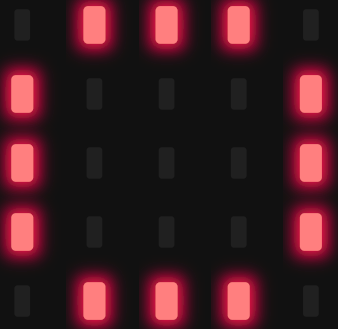
\includegraphics[width=3in]{source/picture/bai_1/pic4.PNG}
    \caption{\textit{12 LEDs for an analog clock}}
    \label{bai1_pic3}
\end{figure}

Report 1: Present the schematic.
\begin{figure}[!htp]
    \centering
    \includegraphics[width=5in]{source/Image/bai6.png}
\end{figure}
Report 2: Implement a simple program to test the connection of every single LED. This testing program should turn every LED in a sequence.
\begin{lstlisting}
  int counter = 12;
  int reset_counter = 12;
  unsigned int hex_num = 0x10;
  while (1)
  {
	  if (counter <= 0) {
		  counter = reset_counter;
		  hex_num = 0x10;
	  }
	  GPIOA->ODR = hex_num;
	  hex_num = hex_num << 1;
	  counter--;
	  HAL_Delay(1000);
    /* USER CODE END WHILE */

    /* USER CODE BEGIN 3 */
  }
\end{lstlisting}

\subsection{Exercise 7}
Implement a function named \textbf{clearAllClock()} to turn off all 12 LEDs. Present the source code of this function.

\begin{lstlisting}[caption=Function Implementation]
unsigned char status[12] = {};
void clearAllClock() {
	GPIOA->ODR = 0x0000;
	for (int i = 0; i < 11; i++) {
		status[i] = 0;
	}
}
\end{lstlisting}

\subsection{Exercise 8}
Implement a function named \textbf{setNumberOnClock(int num)}. The input for this function is from \textbf{0 to 11} and an appropriate LED is turn on. Present the source code of this function.
\begin{lstlisting}
unsigned char status[12] = {};
unsigned int buffer = 0x0000;
void setNumberOnClock(int num) {
	if (num < 0 || num > 11) {
		return;
	}
	if (status[num] == 0) {
		unsigned int hex_num = 0x10 << num;
		buffer += hex_num;
		status[num] = 1;
		GPIOA->ODR = buffer;
	}
}
\end{lstlisting}

\subsection{Exercise 9}
Implement a function named \textbf{clearNumberOnClock(int num)}. The input for this function is from \textbf{0 to 11} and an appropriate LED is turn off. 
\begin{lstlisting}
unsigned char status[12] = {};
unsigned int buffer = 0x0000;
void clearNumberOnClock(int num) {
	if (num < 0 || num > 11) {
		return;
	}
	if (status[num] == 1) {
		unsigned int hex_num = 0x10 << num;
		buffer -= hex_num;
		status[num] = 0;
		GPIOA->ODR = buffer;
	}
}
\end{lstlisting}

\subsection{Exercise 10}
Integrate the whole system and use 12 LEDs to display a clock. At a given time, there are only 3 LEDs are turn on for hour, minute and second information.
\begin{lstlisting}
unsigned char status[12] = {};
unsigned int buffer = 0x0000;
void clearAllClock() {
	GPIOA->ODR = 0x0000;
	buffer = 0x0000;
	for (int i = 0; i < 12; i++) {
		status[i] = 0;
	}
}
void setNumberOnClock(int num) {
	if (num < 0 || num > 11) {
		return;
	}
	if (status[num] == 0) {
		unsigned int hex_num = 0x10 << num;
		buffer += hex_num;
		status[num] = 1;
		GPIOA->ODR = buffer;
	}
}
void clearNumberOnClock(int num) {
	if (num < 0 || num > 11) {
		return;
	}
	if (status[num] == 1) {
		unsigned int hex_num = 0x10 << num;
		buffer -= hex_num;
		status[num] = 0;
		GPIOA->ODR = buffer;
	}
}
  GPIOA->ODR = 0x0000;
  unsigned char second = 0, minute = 0, hour = 0;
  while (1)
  {
	  second++;
	  if (second == 60) {
		  second = 0;
		  minute++;
	  }
	  if (minute == 60) {
		  minute = 0;
		  hour++;
	  }
	  if (hour == 12) {
		  hour = 0;
	  }
	  clearAllClock();
	  setNumberOnClock(second / 5);
	  setNumberOnClock(minute / 5);
	  setNumberOnClock(hour);
	  HAL_Delay(1000);
    /* USER CODE END WHILE */

    /* USER CODE BEGIN 3 */
  }
\end{lstlisting}
\chap{Timer Interrupt and LED Scanning}

\section{Introduction}
Timers are one of the most important features in modern micro-controllers. They allow us to measure how long something takes to execute, create non-blocking code, precisely control pin timing, and even run operating systems. In this manual, how to configure a timer using STM32CubeIDE is presented how to use them to flash an LED. Finally, students are proposed to finalize 10 exercises using timer interrupt for applications based LED Scanning.

\begin{figure}[!htp]
    \centering
    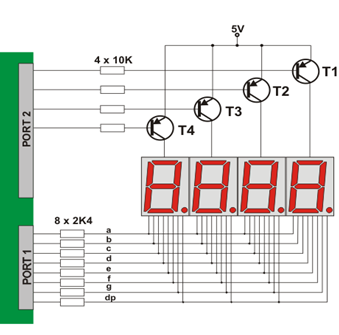
\includegraphics[width=3.5in]{source/picture/bai_2/led_scanning1.png}
    \caption{\textit{Four seven segment LED interface for a micro-controller}}
    \label{bai2_intro1}
\end{figure}


Design an interface for with multiple LED (seven segment or matrix) displays which is to be controlled is depends on the number of input and output pins needed for controlling all the LEDs in the given matrix display, the amount of current that each pin can source and sink and the speed at which the micro-controller can send out control signals. With all these specifications, interfacing can be done for 4 seven segment LEDs with a micro-controller is proposed in the figure above. \\


In the above diagram each seven segment display is having 8 internal LEDs, leading to the total number of LEDs is 32. However, not all the LEDs are required to turn ON, but one of them is needed. Therefore, only 12 lines are needed to control the whole 4 seven segment LEDs.   By controlling with the micro-controller, we can turn ON an LED during a same interval \textbf{$T_S$}. Therfore, the period for controlling all 4 seven segment LEDs is \textbf{$4T_S$}. In other words, these LEDs are scanned at frequecy \textbf{$f = 1 / 4T_S$}. Finally, it is obviously that if the frequency is greater than 30Hz (e.g. f = 50Hz), it seems that all LEDs are turn ON at the same time.\\

In this manual, the timer interrupt is used to design the interval $T_S$ for LED scanning. Unfortunately, the simulation on Proteus can not execute at high frequency, the frequency $f$ is set to a low value (e.g. 1Hz). In a real implementation, this frequency should be 50Hz.


\newpage
\section{Timer Interrupt Setup}
\textbf{Step 1: } Create a simple project, which LED connected to PA5. The manual can be found in the first lab.\\

\textbf{Step 2: } Check the clock source of the system on the tab \textbf{Clock Configuration} (from *.ioc file). In the default configuration, the internal clock source is used with 8MHz, as shown in the figure bellow.

\begin{figure}[!htp]
    \centering
    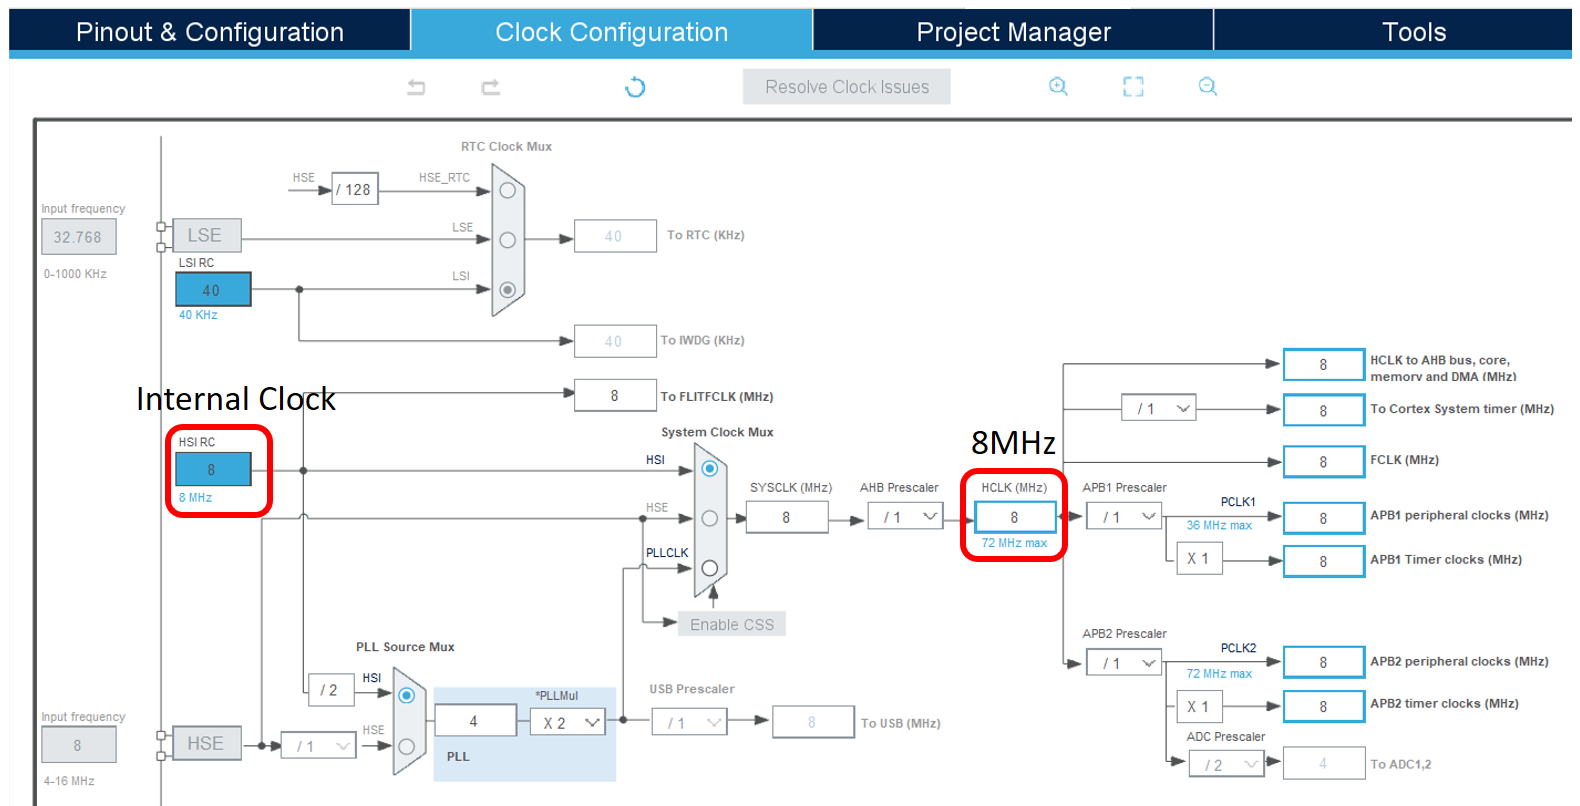
\includegraphics[width=5.5in]{source/picture/bai_2/lab2_m1.PNG}
    \caption{\textit{Default clock source for the system}}
    \label{bai2_m1}
\end{figure}

\textbf{Step 3: } Configure the timer on the \textbf{Parameter Settings}, as follows:
\begin{figure}[!htp]
    \centering
    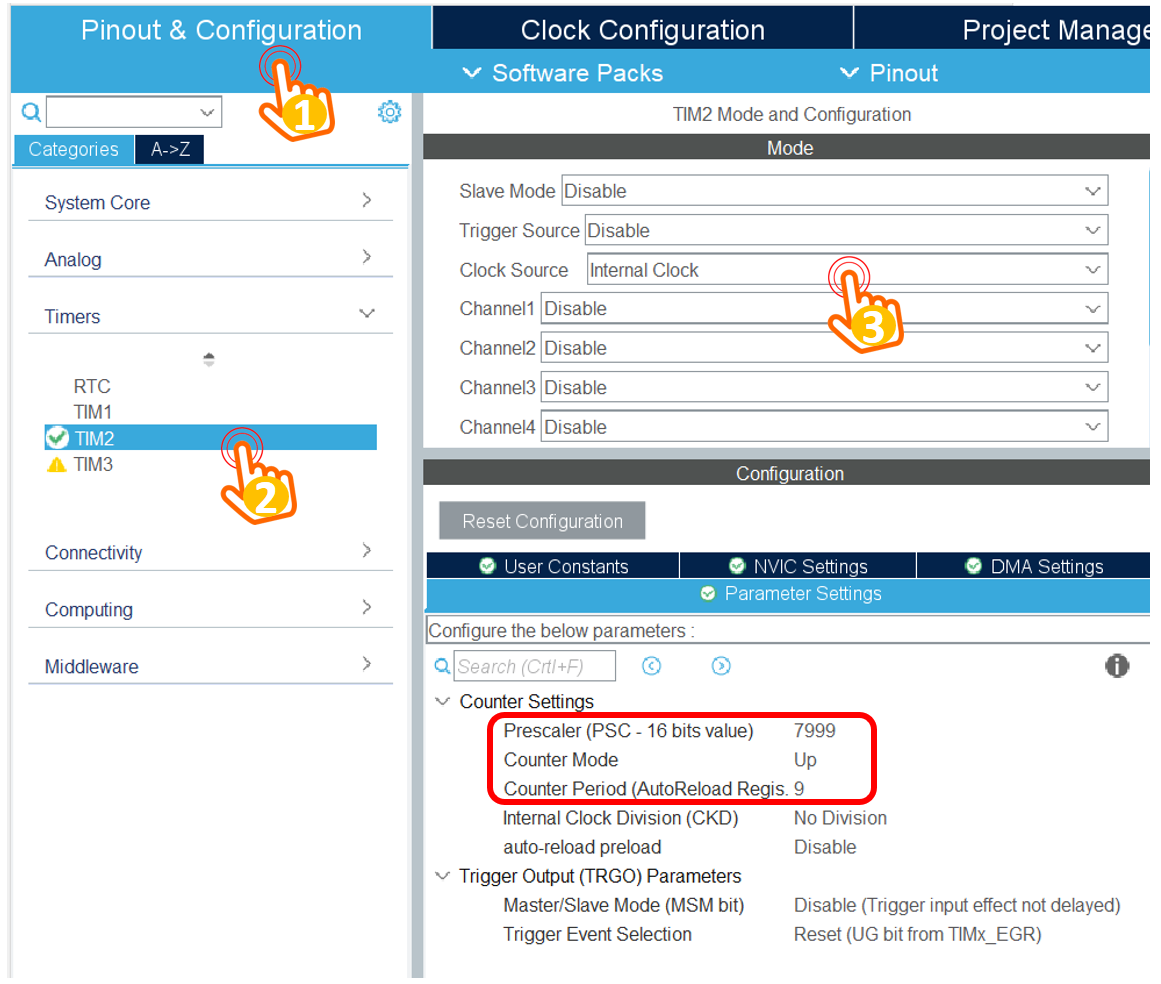
\includegraphics[width=3.5in]{source/picture/bai_2/lab2_m2.PNG}
    \caption{\textit{Configure for Timer 2}}
    \label{bai2_m2}
\end{figure}

Select the clock source for timer 2 to the \textbf{Internal Clock}. Finally, set the prescaller and the counter to 7999 and 9, respectively. These values are explained as follows:
\begin{itemize}
    \item The target is to set an interrupt timer to 10ms
    \item The clock source is 8MHz, by setting the prescaller to 7999, the input clock source to the timer is \textbf{8MHz/(7999+1) = 1000Hz}.
    \item The interrupt is raised when the timer counter is counted from 0 to 9, meaning that the frequency is divided by 10, which is 100Hz.
    \item The frequency of the timer interrupt is 100Hz, meaning that the period is \textbf{1/100Hz = 10ms}.
\end{itemize}

\textbf{Step 4: } Enable the timer interrupt by switching to \textbf{NIVC Settings} tab, as follows:

\begin{figure}[!htp]
    \centering
    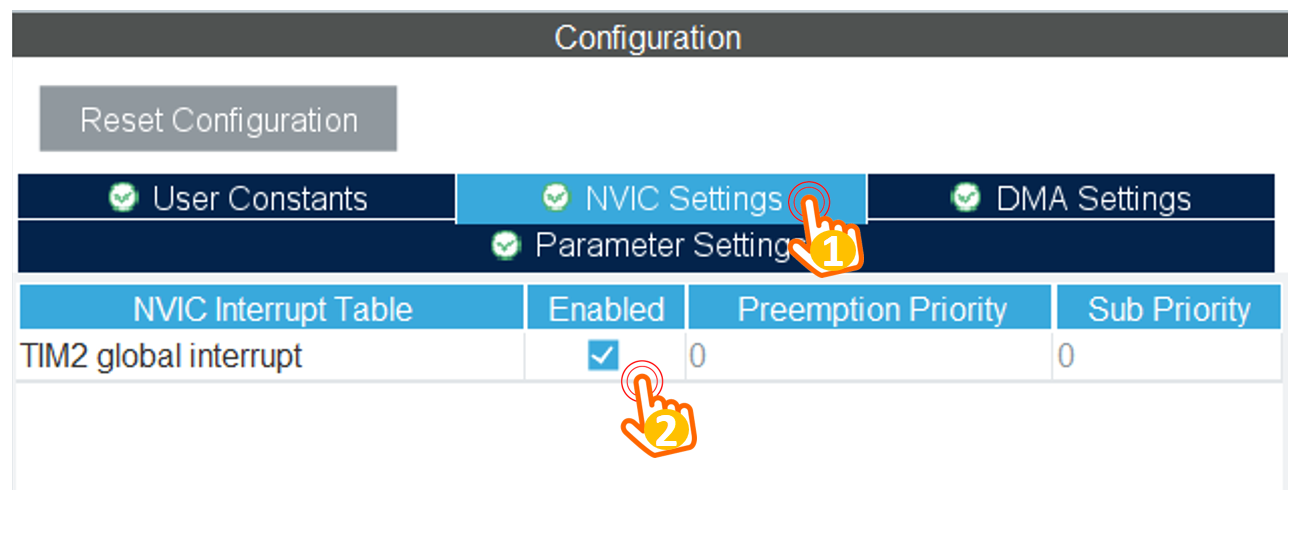
\includegraphics[width=4in]{source/picture/bai_2/lab2_m3.PNG}
    \caption{\textit{Enable timer interrupt}}
    \label{bai2_m3}
\end{figure}

Finally, save the configuration file to generate the source code.\\

\textbf{Step 5: } On the \textbf{main()} function, call the timer init function, as follows:

\begin{lstlisting}[caption=Init the timer interrupt in main]
int main(void)
{
  HAL_Init();
  SystemClock_Config();

  MX_GPIO_Init();
  MX_TIM2_Init();
  
  /* USER CODE BEGIN 2 */
  HAL_TIM_Base_Start_IT(&htim2);
  /* USER CODE END 2 */g3

  while (1){
  
  }
}
\end{lstlisting}

Please put the init function in a right place to avoid conflicts when code generation is executed (e.g. ioc file is updated).\\
\newpage
\textbf{Step 6: } Add the interrupt service routine function, this function is invoked every 10ms, as follows:

\begin{lstlisting}[caption=Add an interrupt service routine]
/* USER CODE BEGIN 4 */
void HAL_TIM_PeriodElapsedCallback(TIM_HandleTypeDef *htim){
	
}
/* USER CODE END 4 */
\end{lstlisting}

\textbf{Step 7: } To run a LED Blinky demo using interrupt, a short manual is presented as follows:
\begin{lstlisting}[caption=LED Blinky using timer interrupt]
/* USER CODE BEGIN 4 */
int counter = 100;
void HAL_TIM_PeriodElapsedCallback(TIM_HandleTypeDef *htim){
	counter--;
	if(counter <= 0){
		counter = 100;
		HAL_GPIO_TogglePin(LED_RED_GPIO_Port, LED_RED_Pin);
	}
}
/* USER CODE END 4 */
\end{lstlisting}

The \textbf{HAL\_TIM\_PeriodElapsedCallback} function is an infinite loop, which is invoked every cycle of the timer 2, in this case, is 10ms.\\



\newpage
\section{Exercise and Report}
\subsection{Exercise 1}
The first exercise show how to interface for multiple seven segment LEDs to STM32F103C6 micro-controller (MCU). Seven segment displays are common anode type, meaning that the anode of all LEDs are tied together as a single terminal and cathodes are left alone as individual pins. \\

In order to save the resource of the MCU, individual cathode pins from all the seven segment LEDs are connected together, and connect to 7 pins of the MCU. These pins are popular known as the \textbf{signal pins}. Meanwhile, the anode pin of each seven segment LEDs are controlled under a power enabling circuit, for instance, an PNP transistor. At a given time, only one seven segment LED is turned on. However, if the delay is small enough, it seems that all LEDs are enabling. \\

Implement the circuit simulation in Proteus with two 7-SEGMENT LEDs as following:

\begin{figure}[!htp]
    \centering
    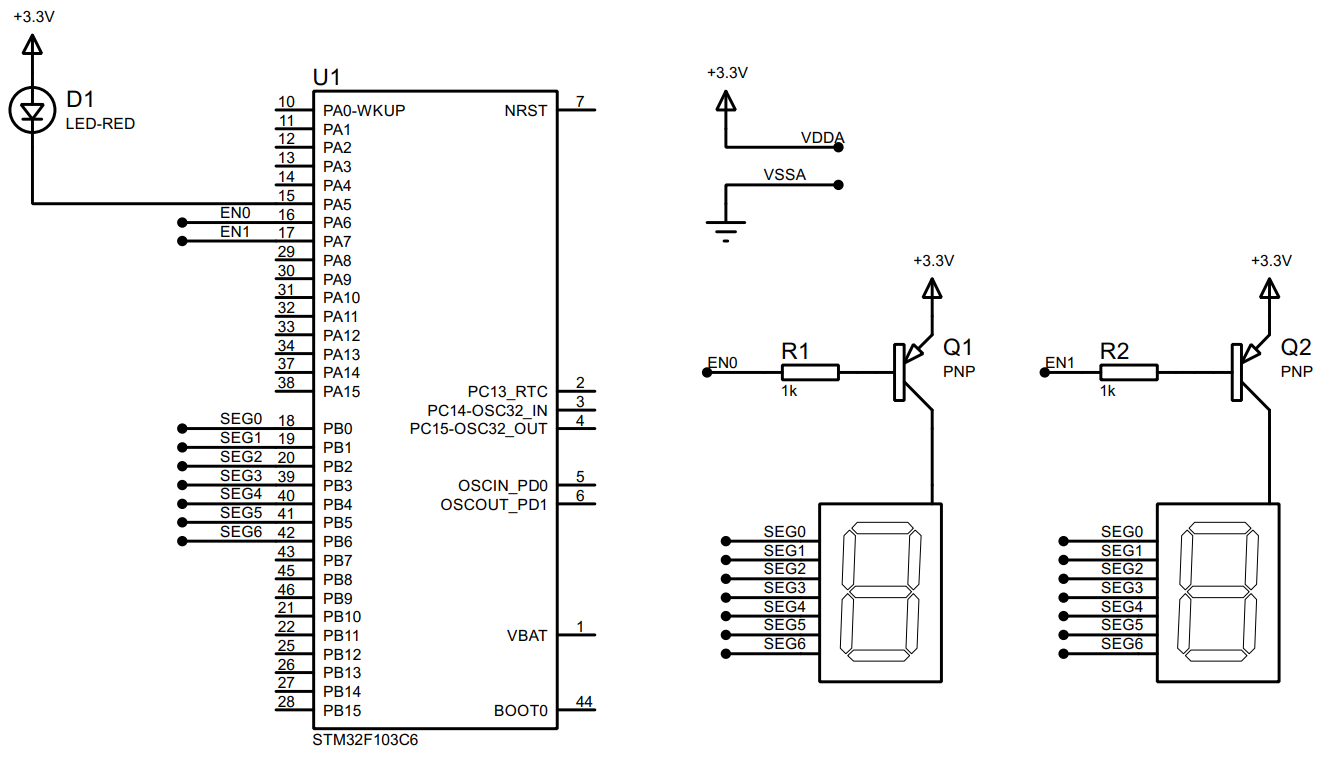
\includegraphics[width=5.5in]{source/picture/bai_2/lab2_ex1a.PNG}
    \caption{\textit{Simulation schematic in Proteus}}
    \label{bai2_pic1a}
\end{figure}
Components used in the schematic are listed bellow:
\begin{itemize}
    \item 7SEG-COM-ANODE (connected from PB0 to PB6)
    \item LED-RED
    \item PNP
    \item RES
    \item STM32F103C6
\end{itemize}


Students are proposed to use the function \textbf{display7SEG(int num)} in the Lab 1 in this exercise. Implement the source code in the interrupt callback function to display number \textbf{"1"} on the first seven segment and number \textbf{"2"} for second one. The switching time between 2 LEDs is half of second. \\

\textbf{Report 1: } Capture your schematic from Proteus and show in the report.\\

\textbf{Report 2: } Present your source code in the \textbf{HAL\_TIM\_PeriodElapsedCallback} function.\\

\textbf{Short question: } What is the frequency of the scanning process?\\

\subsection{Exercise 2}
Extend to 4 seven segment LEDs and two LEDs (connected to PA4, labeled as \textbf{DOT}) in the middle as following:

\begin{figure}[!htp]
    \centering
    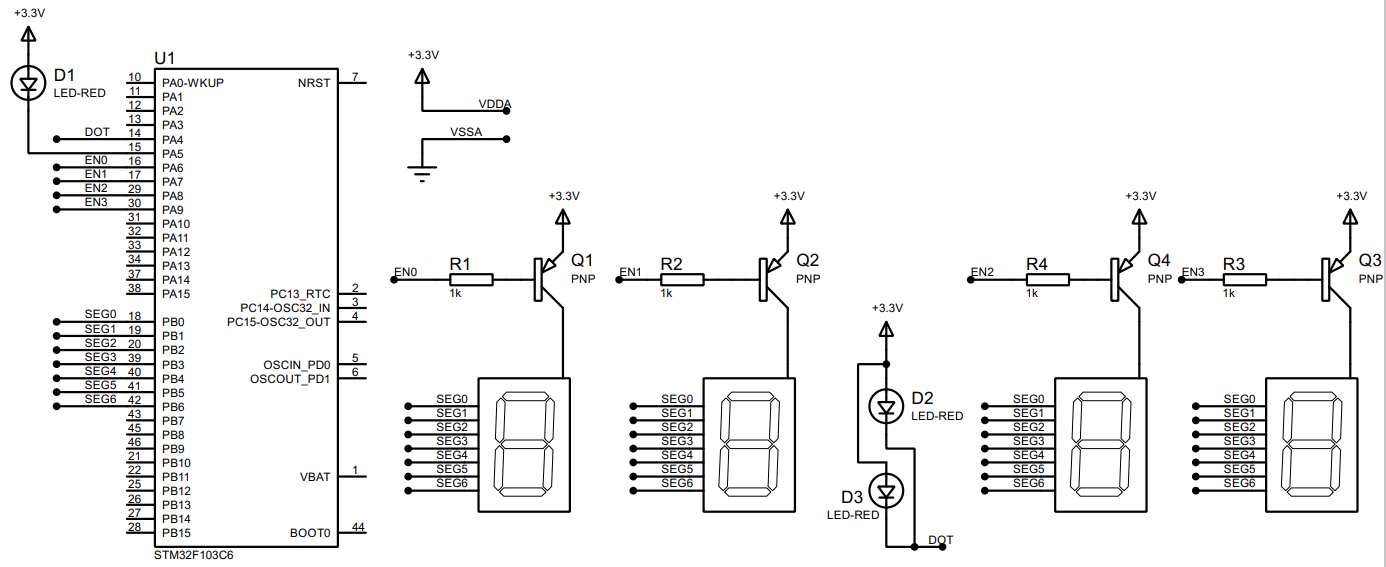
\includegraphics[width=5.5in]{source/picture/bai_2/lab2_ex2a.PNG}
    \caption{\textit{Simulation schematic in Proteus}}
    \label{bai2_pic1a}
\end{figure}

Blink the two LEDs every second. Meanwhile, number 3 is displayed on the third seven segment and number 0 is displayed on the last one (to present 12 hour and a half). The switching time for each seven segment LED is also a half of second (500ms). \textbf{Implement your code in the timer interrupt function.}\\

\textbf{Report 1: } Capture your schematic from Proteus and show in the report.\\

\textbf{Report 2: } Present your source code in the \textbf{HAL\_TIM\_PeriodElapsedCallback} function.\\

\textbf{Short question: } What is the frequency of the scanning process?\\

\subsection{Exercise 3}
Implement a function named \textbf{update7SEG(int index)}. An array of 4 integer numbers are declared in this case. The code skeleton in this exercise is presented as following:
\newpage
\begin{lstlisting}[caption=An example for your source code]
const int MAX_LED = 4;
int index_led = 0;
int led_buffer[4] = {1, 2, 3, 4};
void update7SEG(int index){
    switch (index){
        case 0:
            //Display the first 7SEG with led_buffer[0]
            break;
        case 1:
            //Display the second 7SEG with led_buffer[1]
            break;
        case 2:
            //Display the third 7SEG with led_buffer[2]
            break;
        case 3:
            //Display the forth 7SEG with led_buffer[3]
            break;
        default:
            break;
    }
}
\end{lstlisting}

This function should be invoked in the timer interrupt, e.g update7SEG(index\_led++). The variable \textbf{index\_led} is updated to stay in a valid range, which is from 0 to 3. \\

\textbf{Report 1: } Present the source code of the update7SEG function. \\

\textbf{Report 2: } Present the source code in the HAL\_TIM\_PeriodElapsedCallback.\\

Students are proposed to change the values in the \textbf{led\_buffer} array for unit test this function, which is used afterward.

\subsection{Exercise 4}
Change the period of invoking update7SEG function in order to set the frequency of 4 seven segment LEDs to 1Hz. The DOT is still blinking every second.\\


\textbf{Report 1: } Present the source code in the \textbf{HAL\_TIM\_PeriodElapsedCallback}. \\

\subsection{Exercise 5}
Implement a digital clock with \textbf{hour} and \textbf {minute} information displayed by 2 seven segment LEDs. The code skeleton in the \textbf{main} function is presented as follows:
\begin{lstlisting}[caption=An example for your source code]
int hour = 15, minute = 8, second = 50;

while(1){
    second++;
    if (second >= 60){
        second = 0;
        minute++;
    }
    if(minute >= 60){
        minute = 0;
        hour++;
    }
    if(hour >=24){
        hour = 0;
    }
    updateClockBuffer();
    HAL_Delay(1000);
}
\end{lstlisting}

The function \textbf{updateClockBuffer} will generate values for the array \textbf{led\_buffer} according to the values of hour and minute. In the case these values are 1 digit number, digit 0 is added. \\

\textbf{Report 1: } Present the source code in the \textbf{updateClockBuffer} function.

\subsection{Exercise 6}
The main target from this exercise to reduce the complexity (or reduce code processing) in the timer interrupt. The time consumed in the interrupt can lead to the nested interrupt issue, which can crash the whole system. A simple solution can disable the timer whenever the interrupt occurs, the enable it again. However, the real-time processing is not guaranteed anymore.\\

In this exercise, a software timer is created and its counter is count down every timer interrupt is raised (every 10ms). By using this timer, the \textbf{Hal\_Delay(1000)} in the main function is removed. In a MCU system, non-blocking delay is better than blocking delay. The details to create a software timer are presented bellow. The source code is added to your current program, \textbf{do not delete the source code you have on Exercise 5.}\\

\textbf{Step 1: } Declare variables and functions for a software timer, as following:
\begin{lstlisting}[caption=Software timer based timer interrupt]
/* USER CODE BEGIN 0 */
int timer0_counter = 0;
int timer0_flag = 0;
int TIMER_CYCLE = 10;
void setTimer0(int duration){
	timer0_counter = duration /TIMER_CYCLE;
	timer0_flag = 0;
}
void timer_run(){
	if(timer0_counter > 0){
		timer0_counter--;
		if(timer0_counter == 0) timer0_flag = 1;
	}
}
/* USER CODE END 0 */
\end{lstlisting}

Please change the \textbf{TIMER\_CYCLE} to your timer interrupt period. In the manual code above, it is \textbf{10ms}. \\

\textbf{Step 2: } The \textbf{timer\_run()} is invoked in the timer interrupt as following:

\begin{lstlisting}[caption=Software timer based timer interrupt]
void HAL_TIM_PeriodElapsedCallback(TIM_HandleTypeDef *htim){
	
	timer_run();
	
	//YOUR OTHER CODE
}
\end{lstlisting}

\textbf{Step 3: } Use the timer in the main function by invoked setTimer0 function, then check for its flag (timer0\_flag). An example to blink an LED connected to PA5 using software timer is shown as follows:
\begin{lstlisting}[caption=Software timer is used in main fuction to blink the LED]
setTimer0(1000);
while (1){
    if(timer0_flag == 1){
        HAL_GPIO_TogglePin(LED_RED_GPIO_Port, LED_RED_Pin);
        setTimer0(2000);
    }
}
\end{lstlisting}

\textbf{Report 1: } if in line 1 of the code above is miss, what happens after that and why?\\


\textbf{Report 2: } if in line 1 of the code above is changed to setTimer0(1), what happens after that and why?\\

\textbf{Report 3: } if in line 1 of the code above is changed to setTimer0(10), what is changed compared to 2 first questions and why?\\

\subsection{Exercise 7}
Upgrade the source code in Exercise 5 (update values for hour, minute and second) by using the software timer and remove the HAL\_Delay function at the end. Moreover, the DOT (connected to PA4) of the digital clock is also moved to main function. \\

\textbf{Report 1: } Present your source code in the while loop on main function.

\subsection{Exercise 8}
Move also the update7SEG() function from the interrupt  timer to the main. Finally, the timer interrupt only used to handle  software timers. All processing (or complex computations) is move to an infinite loop on the main function, optimizing the complexity of the interrupt  handler function.\\

\textbf{Report 1: } Present your source code in the the main function. In the case more extra functions are used (e.g. the second software timer), present them in the report as well.

\subsection{Exercise 9}

This is an extra works for this lab. A LED Matrix is added to the system. A reference design is shown in figure bellow:
\begin{figure}[!htp]
    \centering
    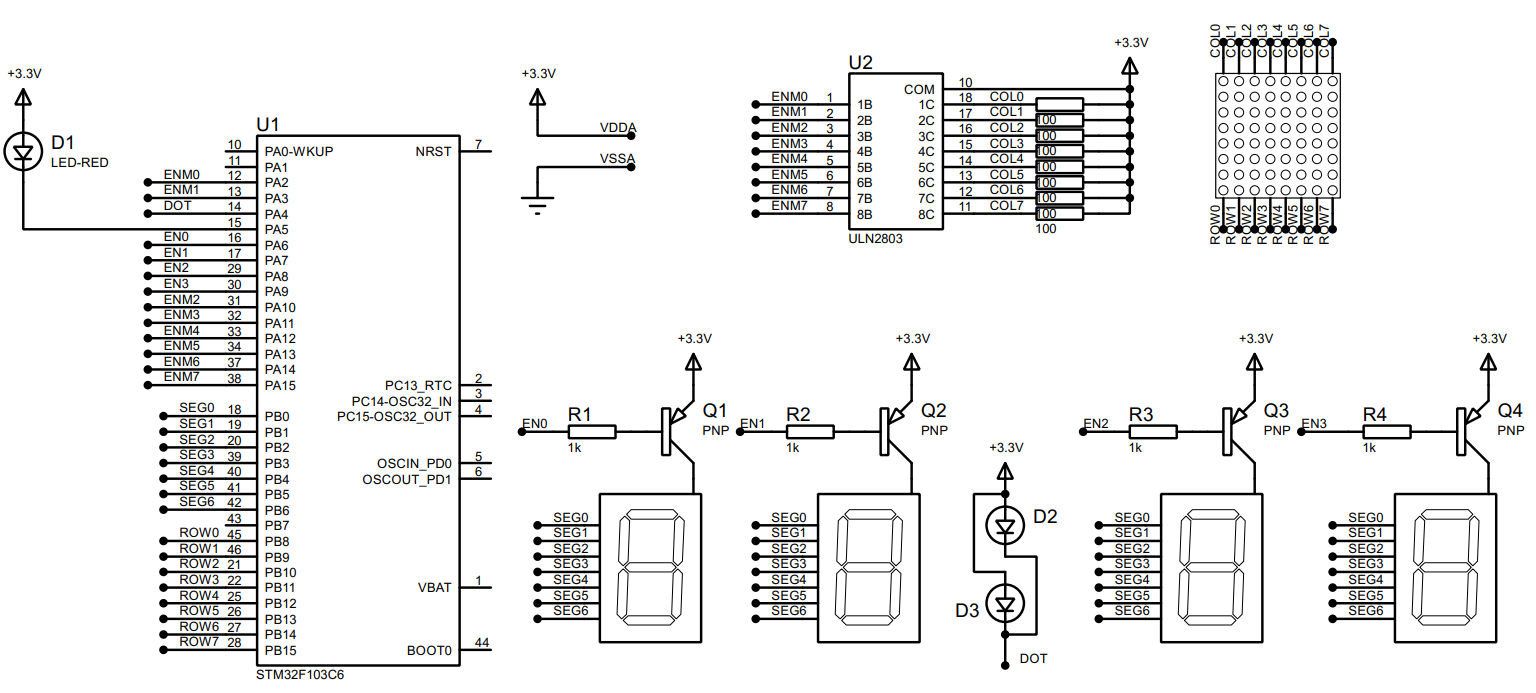
\includegraphics[width=5.5in]{source/picture/bai_2/lab2_m4.PNG}
    \caption{\textit{LED matrix is added to the simulation}}
    \label{bai2_pic9}
\end{figure}

In this schematic, two new components are added, including the \textbf{MATRIX-8X8-RED} and \textbf{ULN2803}, which is an NPN transistor array to enable the power supply for a column of the LED matrix. Students can change the enable signal (from ENM0 to  ENM7) if needed. Finally, the data signal (from ROW0 to ROW7) is connected to PB8 to PB15. \\

\textbf{Report 1: } Present the schematic of your system by capturing the screen in Proteus.\\

\textbf{Report 2: } Implement the function, updateLEDMatrix(int index), which is similarly  to 4 seven led segments.

\begin{lstlisting}[caption=Function to display data on LED Matrix]
const int MAX_LED_MATRIX = 8;
int index_led_matrix = 0;
uint8_t matrix_buffer[8] = {0x01, 0x02, 0x03, 0x04, 0x05, 0x06, 0x07, 0x08};
void updateLEDMatrix(int index){
    switch (index){
        case 0:
            break;
        case 1:
            break;
        case 2:
            break;
        case 3:
            break;
        case 4:
            break;
        case 5:
            break;
        case 6:
            break;
        case 7:
            break;
        default:
            break;
    }
}
\end{lstlisting}

Student are free to choose the invoking frequency of this function. However, this function is supposed to invoked in main function. Finally, please update the \textbf{matrix\_buffer} to display character \textbf{"A"}.

\subsection{Exercise 10}
Create an animation on LED matrix, for example, the character is shifted to the left. 

\textbf{Report 1: } Briefly describe your solution and present your source code in the report.

\chap{Buttons/Switches}


\section{Objectives}
In this lab, you will
\begin{itemize}
    \item Learn how to add new C source files and C header files in an STM32 project, 
    \item Learn how to read digital inputs and display values to LEDs using a timer interrupt of a microcontroller (MCU). 
    \item Learn how to debounce when reading a button.
    \item Learn how to create an FSM and implement an FSM in an MCU.
\end{itemize}

\section{Introduction}
Embedded systems usually use buttons (or keys, or switches, or any form of mechanical contacts) as part of their user interface. This general rule applies from the most basic remote-control system for opening a garage door, right up to the most sophisticated aircraft autopilot system. Whatever the system you create, you need to be able to create a reliable button interface. 

%add a picture of buttons/switch

A button is generally hooked up to an MCU so as to generate a certain logic level when pushed or closed or ``active" and the opposite logic level when unpushed or open or ``inactive."  The active logic level can be either `0' or `1', but for reasons both historical and electrical, an active level of '0' is more common.

We can use a button if we want to perform operations such as:
\begin{itemize}
    \item Drive a motor while a switch is pressed.
    \item Switch on a light while a switch is pressed.
    \item Activate a pump while a switch is pressed.
\end{itemize}
These operations could be implemented using an electrical button without using an MCU; however, use of an MCU may well be appropriate if we require more complex behaviours. For example:
\begin{itemize}
    \item Drive a motor while a switch is pressed. 
    
    \textbf{Condition}: If the safety guard is not in place, don't turn the motor. Instead sound a buzzer for 2 seconds. 
    \item Switch on a light while a switch is pressed.
    
    \textbf{Condition}: To save power, ignore requests to turn on the light during daylight hours. 
    
    \item Activate a pump while a switch is pressed
    
    \textbf{Condition}: If the main water reservoir is below 300 litres, do not start the main pump: instead, start the reserve pump and draw the water from the emergency tank. 
\end{itemize}

In this lab, we consider how you read inputs from mechanical buttons in your embedded application using an MCU. 

% Before considering button/switches themselves, we will consider the process of reading the state of port pins.
\newpage
\section{Basic techniques for reading from port pins}
\subsection{The need for pull-up resistors}
\begin{figure}[!htp]
    \centering
    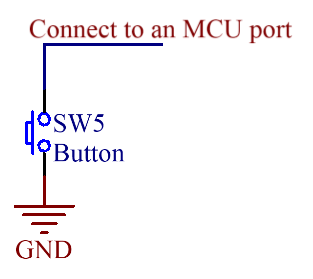
\includegraphics[width=2in]{source/picture/bai_3/Button_Schematic_0.png}
    \caption{\textit{Connecting a button to an MCU}}
    \label{bai4_pic_button_schematic_0}
\end{figure}
Figure \ref{bai4_pic_button_schematic_0} shows a way to connect a button to an MCU. This hardware operates as follows:
\begin{itemize}
    \item When the switch is open, it has no impact on the port pin. An internal resistor on the port ``pulls up" the pin to the supply voltage of the MCU (typically 3.3V for STM32F103). If we read the pin, we will see the value `1'. 
    \item When the switch is closed (pressed), the pin voltage will be 0V. If we read the pin, we will see the value `0'. 
\end{itemize}
 
 However, if the MCU does not have a pull-up resistor inside, when the button is pressed, the read value will be `0', but even we release the button, the read value is still `0' as shown in Figure \ref{bai4_pic_the_need_of_pull_up_resistors}.
 \begin{figure}[!htp]
    \centering
    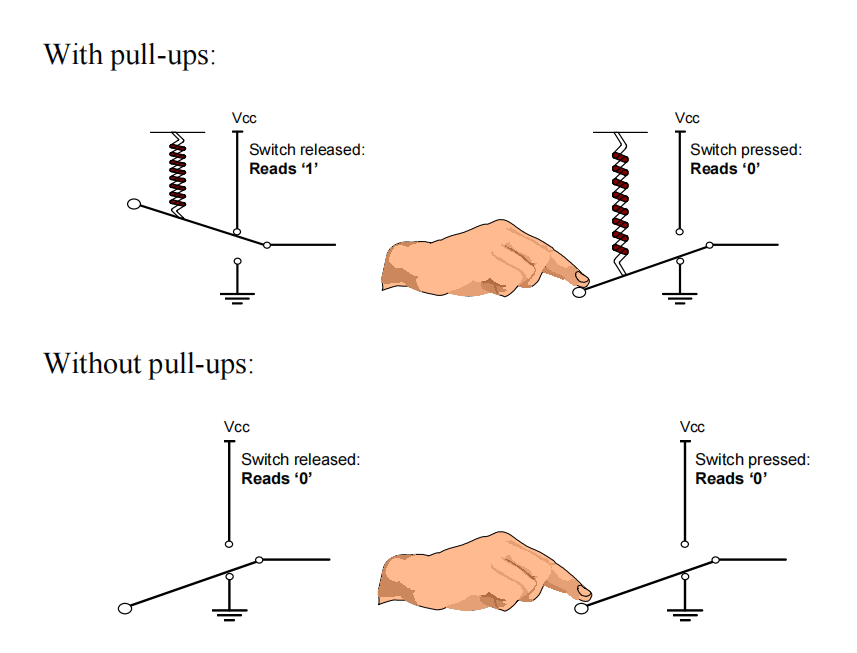
\includegraphics[width=4.5in]{source/picture/bai_3/pullup_resistors.png}
    \caption{\textit{The need of pull up resistors}}
    \label{bai4_pic_the_need_of_pull_up_resistors}
\end{figure}
%add a picture 

So a reliable way to connect a button/switch to an MCU is that we explicitly use an external pull-up resistor as shown in Figure \ref{bai4_pic_button_schematic_1}.

 \begin{figure}[!htp]
    \centering
    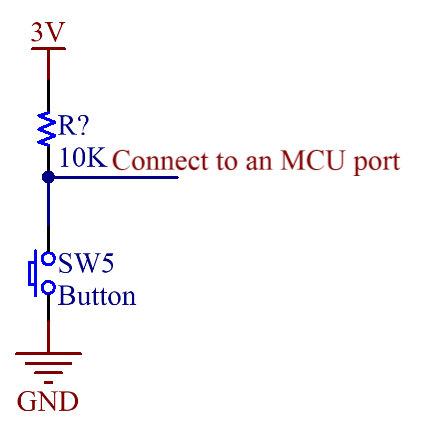
\includegraphics[width=2in]{source/picture/bai_3/Button_Schematic.png}
    \caption{\textit{A reliable way to connect a button to an MCU}}
    \label{bai4_pic_button_schematic_1}
\end{figure}
 
%\newpage 
\subsection{Dealing with switch bounces}
In practice, all mechanical switch contacts bounce (that is, turn on and off, repeatedly, for short period of time) after the switch is closed or opened as shown in Figure \ref{bai4_pic_switchsbounce}.
\begin{figure}[!htp]
    \centering
    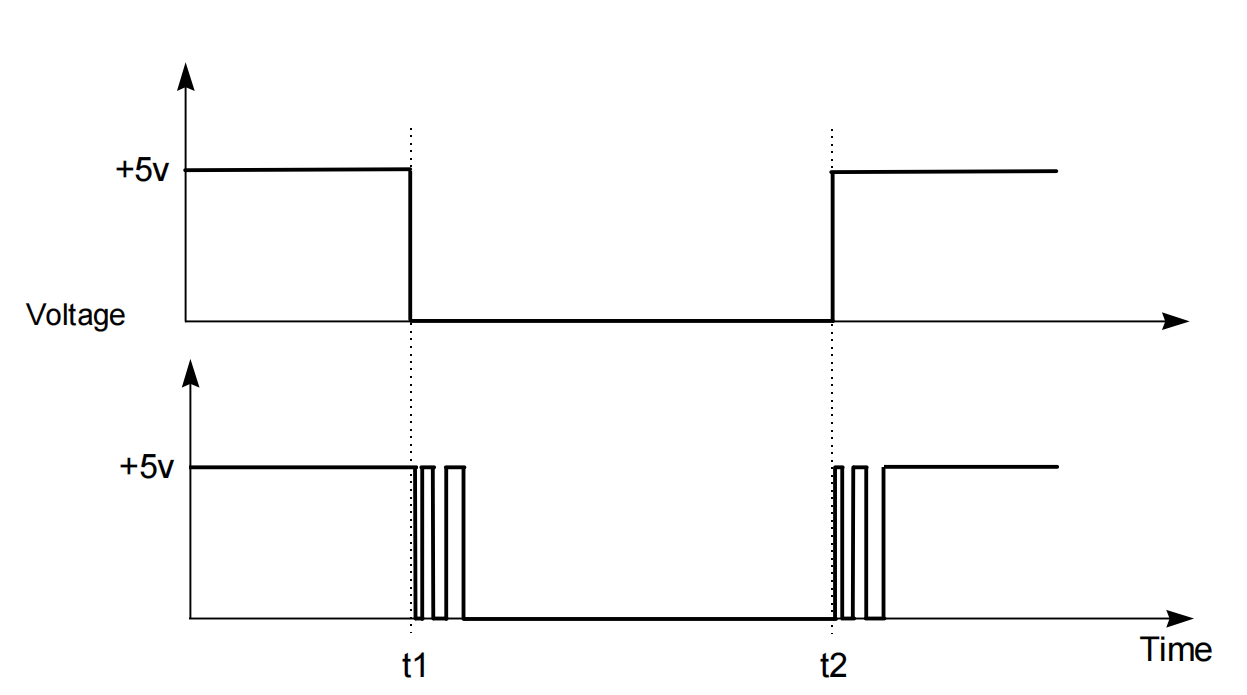
\includegraphics[width=4.5in]{source/picture/bai_3/switchsbounce.png}
    \caption{\textit{Switch bounces}}
    \label{bai4_pic_switchsbounce}
\end{figure}

Every system that uses any kind of mechanical switch must deal with the issue of debouncing.  The key task is to make sure that one mechanical switch or button action is only read as one action by the MCU, even though the MCU will typically be fast enough to detect the unwanted switch bounces and treat them as separate events.  Bouncing can be eliminated by special ICs or by RC circuitry, but in most cases debouncing is done in software because software is ``free".

As far as the MCU concerns, each ``bounce" is equivalent to one press and release of an ``ideal” switch. 
Without appropriate software design, this can give several problems:
\begin{itemize}
    \item Rather than reading ‘A’ from a keypad, we may read ‘AAAAA’
    \item Counting the number of times that a switch is pressed becomes extremely difficult
    \item If a switch is depressed once, and then released some time later, the `bounce' may make it appear as if the switch has been pressed again (at the time of release). 
\end{itemize}


The key to debouncing is to establish a minimum criterion for a valid button push, one that can be implemented in software.  This criterion must involve differences in time - two button presses in 20ms must be treated as one button event, while two button presses in 2 seconds must be treated as two button events.  So what are the relevant times we need to consider?  They are these:
\begin{itemize}
    \item Bounce time:  most buttons seem to stop bouncing within 10ms
    \item Button press time: the shortest time a user can press and release a button seems to be between 50 and 100ms
    \item Response time: a user notices if the system response is 100ms after the button press, but not if it is 50ms after
\end{itemize}



Combining all of these times, we can set a few goals
\begin{itemize}
    \item Ignore all bouncing within 10ms
    \item Provide a response within 50ms of detecting a button push (or release)
    \item Be able to detect a 50ms push and a 50ms release    
\end{itemize}


The simplest debouncing method is to examine the keys (or buttons or switches) every N milliseconds, where N > 10ms (our specified button bounce upper limit) and N <= 50ms (our specified response time).   We then have three possible outcomes every time we read a button:
\begin{itemize}
    \item We read the button in the solid `0' state
    \item We read the button in the solid `1' state
    \item We read the button while it is bouncing (so we will get either a `0' or a `1')
\end{itemize}

Outcomes 1 and 2 pose no problems, as they are what we would always like to happen.  Outcome 3 also poses no problem because during a bounce either state is acceptable.  If we have just pressed an active-low button and we read a '1' as it bounces, the next time through we are guaranteed to read a '0' (remember, the next time through all bouncing will have ceased), so we will just detect the button push a bit later.  Otherwise, if we read a '0' as the button bounces, it will still be '0' the next time after all bouncing has stopped, so we are just detecting the button push a bit earlier.  The same applies to releasing a button.  Reading a single bounce (with all bouncing over by the time of the next read) will never give us an invalid button state.  It's only reading multiple bounces (multiple reads while bouncing is occurring) that can give invalid button states such as repeated push signals from one physical push. 

So if we guarantee that all bouncing is done by the time we next read the button, we're good.  Well, almost good, if we're lucky...

MCUs often live among high-energy beasts, and often control the beasts.  High energy devices make electrical noise, sometimes great amounts of electrical noise.  This noise can, at the worst possible moment, get into your delicate button-and-high-value-pullup circuit and act like a real button push.  Oops, missile launched, sorry!

If the noise is too intense we cannot filter it out using only software, but will need hardware of some sort (or even a redesign).  But if the noise is only occasional, we can filter it out in software without too much bother.  The trick is that instead of regarding a single button `make' or `break' as valid, we insist on N contiguous makes or breaks to mark a valid button event.  N will be a factor of your button scanning rate and the amount of filtering you want to add.  Bigger N gives more filtering.  The simplest filter (but still a big improvement over no filtering) is just an N of 2, which means compare the current button state with the last button state, and only if both are the same is the output valid.

Note that now we have not two but three button states: active (or pressed), inactive (or released), and indeterminate or invalid (in the middle of filtering, not yet filtered).  In most cases we can treat the invalid state the same as the inactive state, since we care in most cases only about when we go active (from whatever state) and when we cease being active (to inactive or invalid).  With that simplification we can look at simple \mathbf{N = 2} filtering reading a button wired to STM32 MCU:
\begin{lstlisting}[caption=Read port pin and deboucing]
void button_reading(void){
    static unsigned char last_button;
    unsigned char raw_button;
    unsigned char filtered_button;
    last_button = raw_button;
    raw_button = HAL_GPIO_ReadPin(BUTTON_1_GPIO_Port, BUTTON_1_Pin);
    if(last_button == raw_button){
        filtered_button = raw_button;
    }
}
\end{lstlisting}

The function button\_reading() must be called no more often than our debounce time (10ms).

To expand to greater filtering (larger N), keep in mind that the filtering technique essentially involves reading the current button state and then either counting or reseting the counter.  We count if the current button state is the same as the last button state, and if our count reaches N we then report a valid new button state.  We reset the counter if the current button state is different than the last button state, and we then save the current button state as the new button state to compare against the next time.  Also note that the larger our value of N the more often our filtering routine must be called, so that we get a filtered response within our specified 50ms deadline.  So for example with an N of 8 we should be calling our filtering routine every 2 - 5ms, giving a response time of 16 - 40ms (>10ms and <50ms).
% Creating a simple software to check for a valid switch input is straightforward:
% \begin{itemize}
%     \item Read the relevant port pin
%     \item If we think we have detected a switch depression, we wait for 50ms and then read the pin again.
%     \item If the second reading confirms the first reading, we assume the switch really has been depressed.
% \end{itemize}

% Note that the figure of ‘50ms’ will depend on the switch used and the deployed environment. 

\newpage
\section{Reading switch input (basic code) using STM32}


To demonstrate the use of buttons/switches in STM32, we use an example which requires to write a program that 
\begin{itemize}
    \item Has a timer which has an interrupt in every 10 milliseconds.  
    \item Reads values of button PB0 every 10 milliseconds. 
    \item Increases the value of LEDs connected to PORTA by one unit when the button PB0 is pressed.
    \item Increases the value of PORTA automatically in every 0.5 second, if the button PB0 is pressed in more than 1 second.

\end{itemize}
\subsection{Input Output Processing Patterns}
For both input and output processing, we have a similar pattern to work with. Normally, we have a module named driver which works directly to the hardware. We also have a buffer to store temporarily values. In the case of input processing, the driver will store the value of the hardware status to the buffer for further processing. In the case of output processing, the driver uses the buffer data to output to the hardware. 

\begin{figure}[!htp]
    \centering
    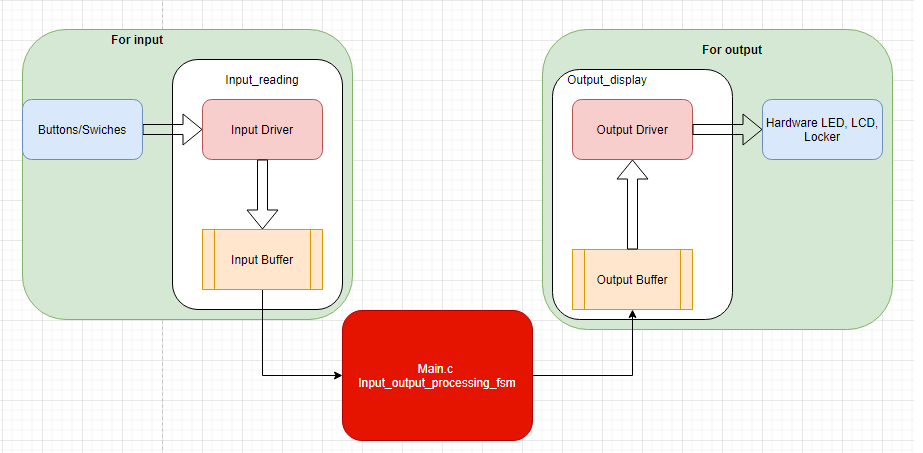
\includegraphics[width=5.5in]{source/picture/bai_3/Input_Output_patterns.png}
    \caption{\textit{Input Output Processing Patterns}}
    \label{bai4_pic_Input_Output_patterns}
\end{figure}

Figure \ref{bai4_pic_Input_Output_patterns} shows that we should have an \emph{input\_reading} module to processing the buttons, then store the processed data to the buffer. Then a module of \emph{input\_output\_processing\_fsm} will process the input data, and update the output buffer. The output driver gets the value from the output buffer to transfer to the hardware. 
\newpage
\subsection{Setting up}
\subsubsection{Create a project}
Please follow the instruction in Labs 1 and 2 to create a project that includes: 
\begin{itemize}
    \item PB0 as an input port pin, 
    \item PA0-PA7 as output port pins, and 
    \item Timer 2 10ms interrupt
\end{itemize}

% \begin{figure}[!htp]
%     \centering
%     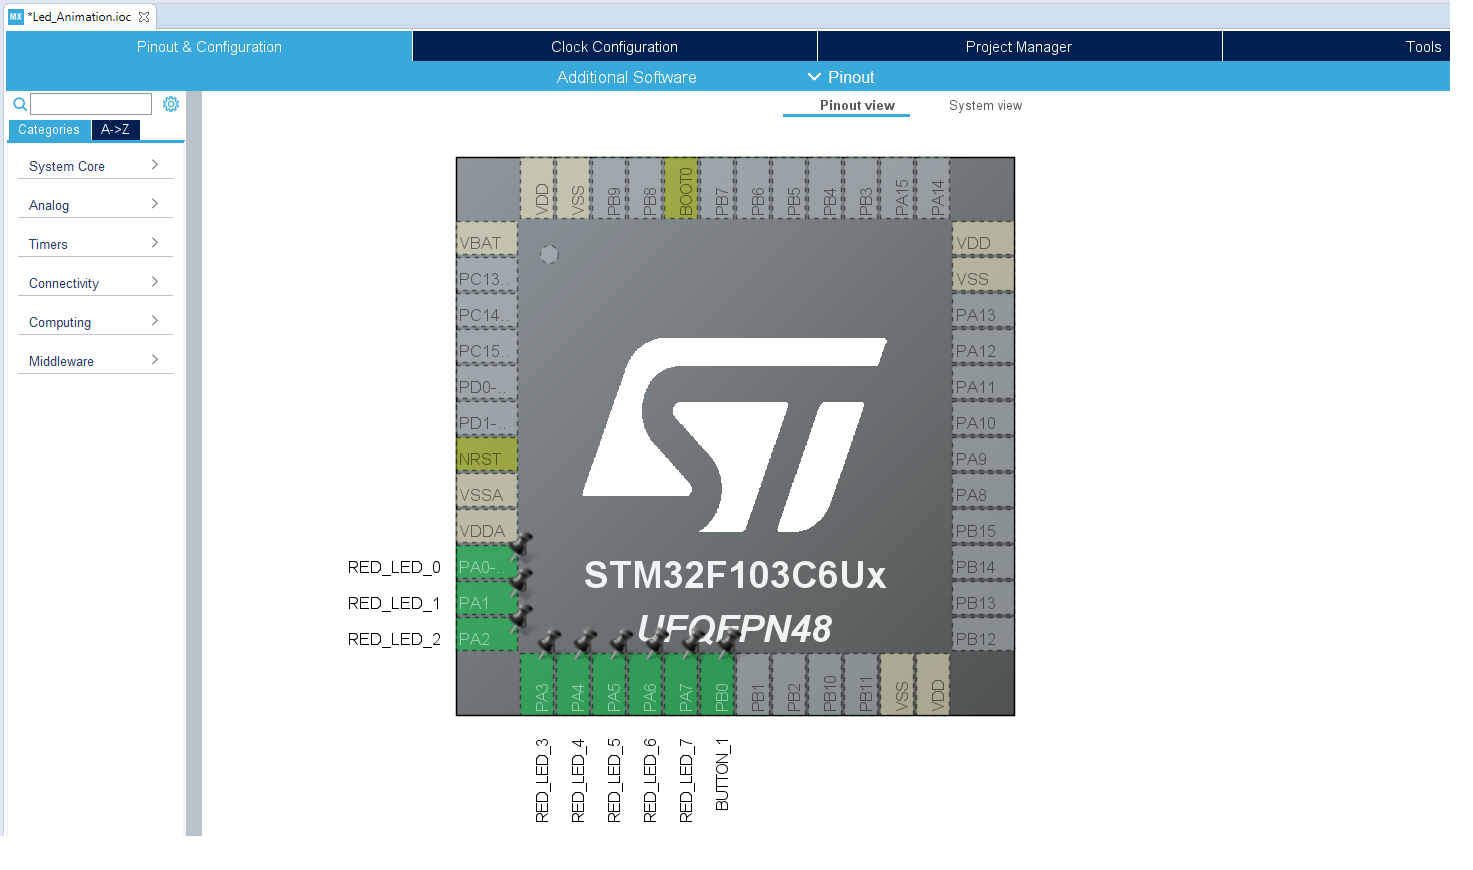
\includegraphics[width=5.5in]{source/picture/bai_3/Input_Output_Settings.png}
%     \caption{\textit{Input Output Setting}}
%     \label{bai4_pic_input_output_setting}
% \end{figure}


\subsubsection{Create a file C source file and header file for input reading}
We are expected to have files for button processing and led display as shown in Figure \ref{bai4_pic_Adding_new_files_to_project}.

\begin{figure}[!htp]
    \centering
    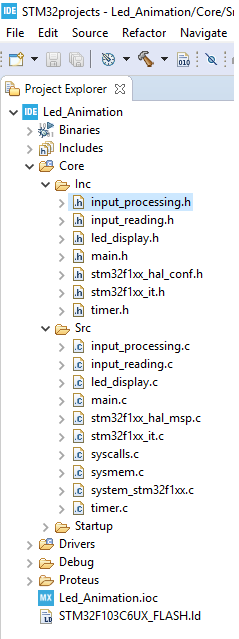
\includegraphics[width=1.5in]{source/picture/bai_3/Adding_new_files_to_project.png}
    \caption{\textit{File Organization}}
    \label{bai4_pic_Adding_new_files_to_project}
\end{figure}

Steps 1 (Figure \ref{bai4_pic_Adding_new_files_to_project_step_1}): Right click to the folder \textbf{Src}, select \textbf{New}, then select \textbf{Source File}. There will be a pop-up. Please type the file name, then click \textbf{Finish}.
\begin{figure}[!htp]
    \centering
    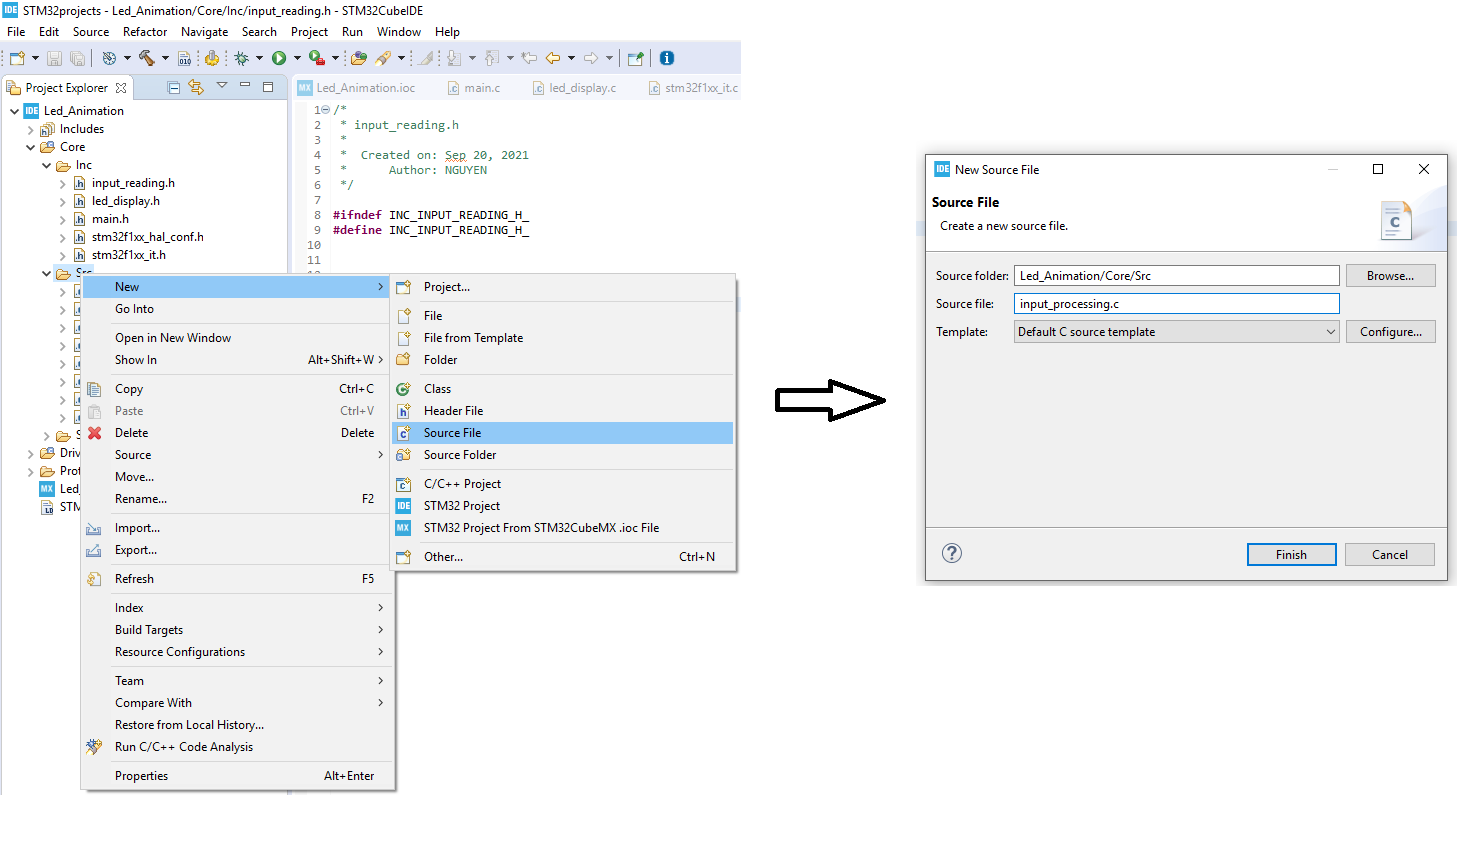
\includegraphics[width=5.5in]{source/picture/bai_3/Adding_new_files_to_project_step_1.png}
    \caption{\textit{Step 1: Create a C source file for input reading}}
    \label{bai4_pic_Adding_new_files_to_project_step_1}
\end{figure}

Step 2 (Figure \ref{bai4_pic_Adding_new_files_to_project_step_3}): Do the same for the C header file in the folder \textbf{Inc}.
\begin{figure}[!htp]
    \centering
    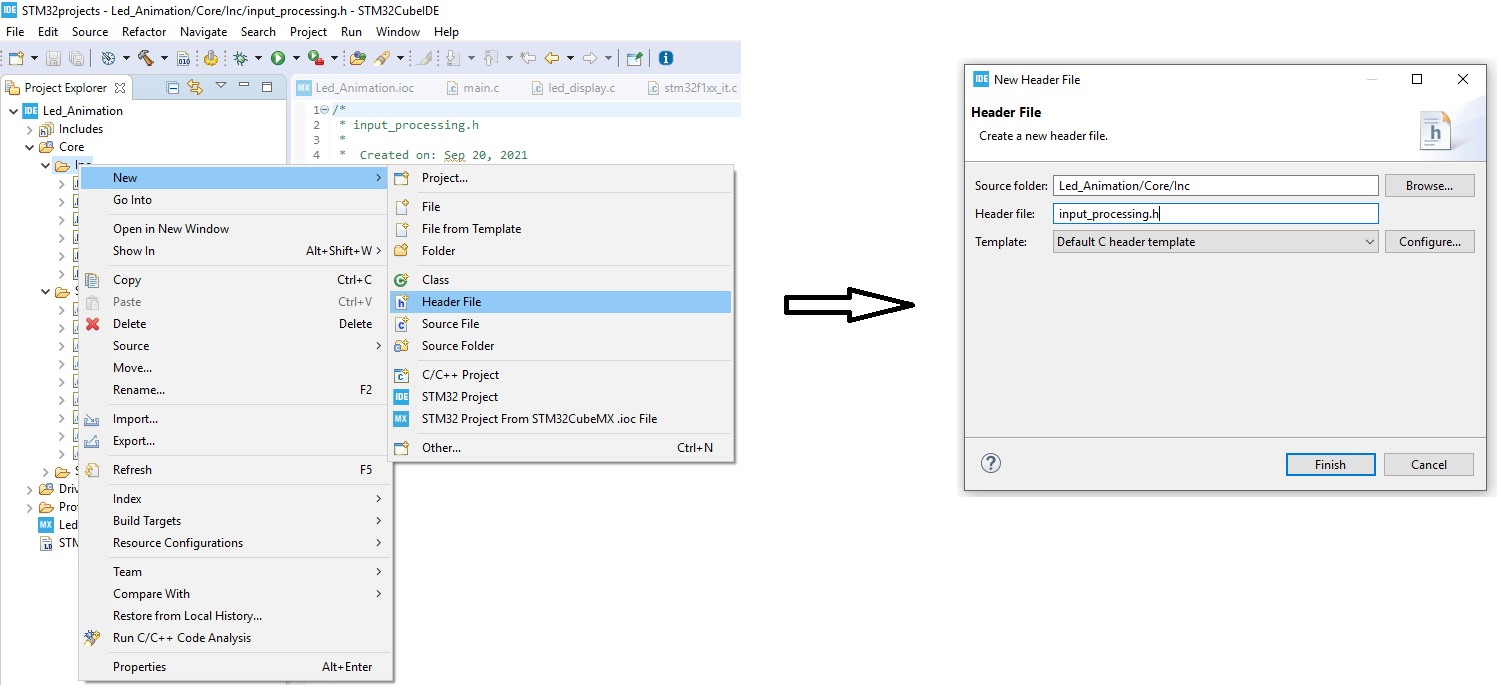
\includegraphics[width=5.5in]{source/picture/bai_3/Adding_new_files_to_project_step_3.png}
    \caption{\textit{Step 2: Create a C header file for input processing}}
    \label{bai4_pic_Adding_new_files_to_project_step_3}
\end{figure}


\newpage

\newpage
\subsection{Code For Read Port Pin and Debouncing}
\subsubsection{The code in the input\_reading.c file}
\begin{lstlisting}[caption=Define constants buffers and button\_reading function]
#include "main.h"
//we aim to work with more than one buttons
#define N0_OF_BUTTONS 				       1
//timer interrupt duration is 10ms, so to pass 1 second, 
//we need to jump to the interrupt service routine 100 time
#define DURATION_FOR_AUTO_INCREASING	   100
#define BUTTON_IS_PRESSED                  GPIO_PIN_RESET
#define BUTTON_IS_RELEASED                 GPIO_PIN_SET
//the buffer that the final result is stored after 
//debouncing
static GPIO_PinState buttonBuffer[N0_OF_BUTTONS];
//we define two buffers for debouncing
static GPIO_PinState debounceButtonBuffer1[N0_OF_BUTTONS];
static GPIO_PinState debounceButtonBuffer2[N0_OF_BUTTONS];
//we define a flag for a button pressed more than 1 second.
static uint8_t flagForButtonPress1s[N0_OF_BUTTONS];
//we define counter for automatically increasing the value 
//after the button is pressed more than 1 second.
static uint16_t counterForButtonPress1s[N0_OF_BUTTONS];
void button_reading(void){
	for(char i = 0; i < N0_OF_BUTTONS; i ++){
		debounceButtonBuffer2[i] =debounceButtonBuffer1[i];
		debounceButtonBuffer1[i] = HAL_GPIO_ReadPin(BUTTON_1_GPIO_Port, BUTTON_1_Pin);
		if(debounceButtonBuffer1[i] == debounceButtonBuffer2[i])
			buttonBuffer[i] = debounceButtonBuffer1[i];
			if(buttonBuffer[i] == BUTTON_IS_PRESSED){
			//if a button is pressed, we start counting
				if(counterForButtonPress1s[i] < DURATION_FOR_AUTO_INCREASING){
					counterForButtonPress1s[i]++;
				} else {
				//the flag is turned on when 1 second has passed 
				//since the button is pressed.
					flagForButtonPress1s[i] = 1;
					//todo
				}
			} else {
				counterForButtonPress1s[i] = 0;
				flagForButtonPress1s[i] = 0;
			}
	}
}
\end{lstlisting}

% The program reads all buttons two consecutive times and compare the values. If the values are the same, update the value to buttonBuffer. This function should be called inside the timer interrupt service routine.
% \begin{lstlisting}[caption=Read port pin and deboucing]
% void button_reading(void){
% 	for(char i = 0; i < N0_OF_BUTTONS; i ++){
% 		debounceButtonBuffer2[i] =debounceButtonBuffer1[i];
% 		debounceButtonBuffer1[i] = HAL_GPIO_ReadPin(BUTTON_1_GPIO_Port, BUTTON_1_Pin);
% 		if(debounceButtonBuffer1[i] == debounceButtonBuffer2[i])
% 			buttonBuffer[i] = debounceButtonBuffer1[i];
% 			if(buttonBuffer[i] == BUTTON_IS_PRESSED){
% 			//if a button is pressed, we start counting
% 				if(counterForButtonPress1s[i] < DURATION_FOR_AUTO_INCREASING){
% 					counterForButtonPress1s[i]++;
% 				} else {
% 				//the flag is turned on when 1 second has passed 
% 				//since the button is pressed.
% 					flagForButtonPress1s[i] = 1;
% 					//todo
% 				}

% 			} else {
% 				counterForButtonPress1s[i] = 0;
% 				flagForButtonPress1s[i] = 0;
% 			}
% 	}
% }
% \end{lstlisting}


\begin{lstlisting}[caption=Checking a button is pressed or not]
unsigned char is_button_pressed(uint8_t index){
	if(index >= N0_OF_BUTTONS) return 0;
	return (buttonBuffer[index] == BUTTON_IS_PRESSED);
}
\end{lstlisting}
\begin{lstlisting}[caption=Checking a button is pressed more than a second or not]
unsigned char is_button_pressed_1s(unsigned char index){
	if(index >= N0_OF_BUTTONS) return 0xff;
	return (flagForButtonPress1s[index] == 1);
}
\end{lstlisting}
\subsubsection{The code in the input\_reading.h file}
\begin{lstlisting}[caption=Prototype in input\_reading.h file]
#ifndef INC_INPUT_READING_H_
#define INC_INPUT_READING_H_
void button_reading(void);
unsigned char is_button_pressed(unsigned char index);
unsigned char is_button_pressed_1s(unsigned char index);
#endif /* INC_INPUT_READING_H_ */
\end{lstlisting}

\subsubsection{The code in the timer.c file}
\begin{lstlisting}[caption=Timer interrupt callback function]
#include "main.h"
#include "input_reading.h"

void HAL_TIM_PeriodElapsedCallback(TIM_HandleTypeDef *htim)
{
	if(htim->Instance == TIM2){
		button_reading();
	}
}

\end{lstlisting}



\newpage
\subsection{Button State Processing}
\subsubsection {Finite State Machine}
To solve the example problem, we define 3 states as follows:
\begin{itemize}
    \item State 0: The button is released or the button is in the initial state. 
    \item State 1: When the button is pressed, the FSM will change to State 1 that is increasing the values of PORTA by one value. If the button is released, the FSM goes back to State 0.
    \item State 2: while the FSM is in State 1, the button is kept pressing more than 1 second, the state of FSM will change from 1 to 2. In this state, if the button is kept pressing, the value of PORTA will be increased automatically in every 500ms. If the button is released, the FSM goes back to State 0.
\end{itemize}
\begin{figure}[!htp]
    \centering
    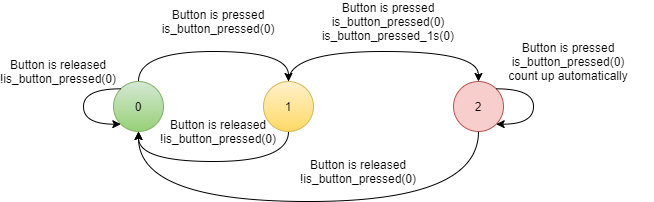
\includegraphics[width=5.5in]{source/picture/bai_3/fsm.png}
    \caption{\textit{An FSM for processing a button}}
    \label{bai4_pic_fsm_for_button_processing}
\end{figure}
\newpage
\subsubsection{The code for the FSM in the input\_processing.c file}
Please note that \emph{fsm\_for\_input\_processing} function should be called inside the super loop of the main functin. 
\begin{lstlisting}[caption=The code in the input\_processing.c file]
#include "main.h"
#include "input_reading.h"

enum ButtonState{BUTTON_RELEASED, BUTTON_PRESSED, BUTTON_PRESSED_MORE_THAN_1_SECOND} ;
enum ButtonState buttonState = BUTTON_RELEASED;
void fsm_for_input_processing(void){
	switch(buttonState){
	case BUTTON_RELEASED:
		if(is_button_pressed(0)){
			buttonState = BUTTON_PRESSED;
			//INCREASE VALUE OF PORT A BY ONE UNIT
		}
		break;
	case BUTTON_PRESSED:
		if(!is_button_pressed(0)){
			buttonState = BUTTON_RELEASED;
		} else {
			if(is_button_pressed_1s(0)){
				buttonState = BUTTON_PRESSED_MORE_THAN_1_SECOND;
			}
		}
		break;
	case BUTTON_PRESSED_MORE_THAN_1_SECOND:
		if(!is_button_pressed(0)){
			buttonState = BUTTON_RELEASED;
		}
		//todo
		break;
	}
}
\end{lstlisting}
\subsubsection{The code in the input\_processing.h}
\begin{lstlisting}[caption=Code in the input\_processing.h file]
#ifndef INC_INPUT_PROCESSING_H_
#define INC_INPUT_PROCESSING_H_

void fsm_for_input_processing(void);

#endif /* INC_INPUT_PROCESSING_H_ */
\end{lstlisting}


\subsubsection{The code in the main.c file}
\begin{lstlisting}[caption=The code in the main.c file]
#include "main.h"
#include "input_processing.h"
//don't modify this part
int main(void){
    HAL_Init();
    /* Configure the system clock */
    SystemClock_Config();
    /* Initialize all configured peripherals */
    MX_GPIO_Init();
    MX_TIM2_Init();
    while (1)
    {
        //you only need to add the fsm function here
        fsm_for_input_processing();
    }
}
\end{lstlisting}

\newpage
\section{Exercises and Report}
\subsection{Specifications}
You are required to build an application of a traffic light in a cross road which includes some features as described below:
\begin{itemize}
    \item The application has 12 LEDs including 4 red LEDs, 4 amber LEDs, 4 green LEDs.
    \item The application has 4 seven segment LEDs to display time with 2 for each road. The 2 seven segment LEDs will show time for each color LED corresponding to each road.
    \item The application has three buttons which are used
    \subitem - to select modes, 
    \subitem - to modify the time for each color led on the fly, and 
    \subitem - to set the chosen value. 
    \item The application has at least 4 modes which is controlled by the first button. Mode 1 is a normal mode, while modes 2 3 4 are  modification modes. You can press the first button to change the mode. Modes will change from 1 to 4 and back to 1 again. 
    
    \textbf{Mode 1 - Normal mode}: 
    \subitem - The traffic light application is running normally.   
    
    \textbf{Mode 2 - Modify time duration for the red LEDs}: This mode allows you to change the time duration of the red LED in the main road. The expected behaviours of this mode include:  
    \subitem - All single red LEDs are blinking in 2 Hz. 
    \subitem - Use two seven-segment LEDs to display the value.
    \subitem - Use the other two seven-segment LEDs to display the mode.
    \subitem - The second button is used to increase the time duration value for the red LEDs. 
    \subitem - The value of time duration is in a range of 1 - 99. 
    \subitem - The third button is used to set the value.
    
    
    \textbf{Mode 3 - Modify time duration for the amber LEDs}: Similar for the red LEDs described above with the amber LEDs.
    
    
    \textbf{Mode 4 - Modify time duration for the green LEDs}: Similar for the red LEDs described above with the green LEDs.
\end{itemize}

\newpage
\subsection{Exercise 1: Sketch an FSM}
Your task in this exercise is to sketch an FSM that describes your idea of how to solve the problem.

Please add your report here.

\subsection{Exercise 2: Proteus Schematic}
Your task in this exercise is to draw a Proteus schematic for the problem above. 

Please add your report here.


\subsection{Exercise 3: Create STM32 Project}
Your task in this exercise is to create a project that has pin corresponding to the Proteus schematic that you draw in previous section. You need to set up your timer interrupt is about 10ms.

Please add your report here.

\subsection{Exercise 4: Modify Timer Parameters}
Your task in this exercise is to modify the timer settings so that when we want to change the time duration of the timer interrupt, we change it the least and it will not affect the overall system. For example, the current system we have implemented is that it can blink an LED in 2 Hz, with the timer interrupt duration is 10ms. However, when we want to change the timer interrupt duration to 1ms or 100ms, it will not affect the 2Hz blinking LED. 

Please add your report here.
\subsection{Exercise 5: Adding code for button debouncing}
Following the example of button reading and debouncing in the previous section, your tasks in this exercise are:
\begin{itemize}
    \item To add new files for input reading and output display,
    \item To add code for button debouncing,
    \item To add code for increasing mode when the first button is pressed. 
\end{itemize}

Please add your report here.
\newpage
\subsection{Exercise 6: Adding code for displaying modes}
Your tasks in this exercise are:
\begin{itemize}
    \item To add code for display mode on seven-segment LEDs, and
    \item To add code for blinking LEDs depending on the mode that is selected. 
\end{itemize}

Please add your report here.
\subsection{Exercise 7: Adding code for increasing time duration value for the red LEDs}
Your tasks in this exercise are: 
\begin{itemize}
    \item to use the second button to increase the time duration value of  the red LEDs
    \item to use the third button to set the value for the red LEDs.
\end{itemize}
Please add your report here.

\subsection{Exercise 8: Adding code for increasing time duration value for the amber LEDs}

Your tasks in this exercise are: 
\begin{itemize}
    \item to use the second button to increase the time duration value of the amber LEDs
    \item to use the third button to set the value for the amber LEDs.
\end{itemize}
Please add your report here.
\subsection{Exercise 9: Adding code for increasing time duration value for the green LEDs}

Your tasks in this exercise are: 
\begin{itemize}
    \item to use the second button to increase the  time duration value of the green LEDs
    \item to use the third button to set the value for the green LEDs.
\end{itemize}
Please add your report here.

\subsection{Exercise 10: To finish the project}
Your tasks in this exercise are:
\begin{itemize}
    \item To integrate all the previous tasks to one final project
    \item To create a video to show all features in the specification
    \item To add a report to describe your solution for each exercise.
    \item To submit your report and code on the BKeL
\end{itemize}

% \section{Problem 1}

% In this week lab, assume you have two button and 8 LEDs, you have to write a program that
% \begin{itemize}
%     \item Has a timer which has an interrupt in every 10 milliseconds.  
%     \item  Reads values of buttons 1 and 2 every 10 milliseconds. The read button function should be called inside the timer interrupt service routine.
%     \item Increases the value of LEDs connected to PORTA when the button 1 is pressed.
%     \item Increases the value of PORTA automatically in every 0.5 second, if the button 1 is pressed in more than 1 second.
%     \item Increases the value of PORTA automatically in every 0.1 second, if the button 1 is pressed in more than 3 seconds.
%     \item Decreases the value of PORTA when the button 2 is pressed
%     \item Decreases the value of PORTA automatically in every 0.5 second, if the button 2 is pressed in more than 1 second.
%     \item Decreases the value of PORTA automatically in every 0.1 second, if the button 2 is pressed in more than 3 seconds.
%     \item The above values such as 10 ms, 0.5 s, 0.1s, 1 s and 3 s are fixed values as an example. Your program, however, needs to provide an easy way to change those values. For example, you should use DEFINE to define those values.
%     \item If both buttons 1 and 2 are pressed, button 1 has a higher priority.
% \end{itemize}


% \section{Problem 2 - A digital clock}
%  You have to write a program that mimics a Casio digital watch. Assume you have 2 buttons and 6 seven-segment LED, a program should have
% \begin{itemize}
%     \item A normal clock that shows hours, minutes, and seconds on 6 seven-segment LEDs.
%     \item  A stopwatch that shows minutes, seconds and 1/100 second
%     \item We use button 1 to change modes of a digital watch. Every time button 1 is pressed, the watch will change to the next mode.
%     \item Mode 0: runs normal clock (default)
%     \item Mode 1: modifies hours. In this mode, the hour number is blinking, and button 2 is used for increasing the hour number.  If button 2 is kept pressed more than 1 second, the hour number will increase automatically, i.e., 5 times per second. Please note that the hour number should be returned to 0 when it reaches 23.
%     \item  Mode 2: modifies minutes. Similar to mode 1, the minute number is blinking and increases when button 2 is pressed.
%     \item Mode 3: modifies seconds. Similar to mode 1, the second number is blinking and increases when button 2 is pressed.
%     \item Mode 4: runs a stopwatch. Using button 2 to start and stop the watch.  
 
% \end{itemize}
%  Please note that while the stopwatch is running, the normal clock is still running in the background.


 

% \section{Instructions}

% Your task is to sketch an FSM that describes your idea of how to solve the above problems and  writes a firmware that runs on STM32.



 

% \section{Submission}

% You need to
% \begin{itemize}
%     \item Demonstrate your work in the lab class and then
%     \item  Submit your FSM sketches and source code to the BKeL.
% \end{itemize}

\chap{Digital Clock Project}
 \chap{A cooperative scheduler}

\section{Introduction}
\subsection{Super Loop Architecture}
\begin{lstlisting}[basicstyle=\small, caption=Super loop program,label = {program_super_loop}]
}
void main(void){
    // Prepare for Task X
    X_Init();
    while(1) {// 'for ever' (Super Loop)
        X(); // Perform the task
    } 
}
\end{lstlisting}
The main advantages of the Super Loop architecture illustrated above are:
\begin{itemize}
    \item (1) that it is simple, and therefore easy to understand, and 
    \item (2) that it consumes virtually no system memory or CPU resources.
\end{itemize}

However, we get ‘nothing for nothing’: Super Loops consume little memory or
processor resources because they provide few facilities to the developer. A particular
limitation with this architecture is that it is very difficult to execute Task X at precise
intervals of time: as we will see, this is a very significant drawback.

For example, consider a collection of requirements assembled from a range of different embedded projects (in no particular order):
\begin{itemize}
    \item The current speed of the vehicle must be measured at 0.5 second intervals.
    \item The display must be refreshed 40 times every second. 
    \item The calculated new throttle setting must be applied every 0.5 seconds.
    \item A time-frequency transform must be performed 20 times every second.
    \item If the alarm sounds, it must be switched off (for legal reasons) after 20 minutes.
    \item If the front door is opened, the alarm must sound in 30 seconds if the correct
password is not entered in this time.    
\item The engine vibration data must be sampled 1,000 times per second.
    \item The frequency-domain data must be classified 20 times every second.
    \item The keypad must be scanned every 200 ms.
    \item The master (control) node must communicate with all other nodes (sensor nodes
and sounder nodes) once per second.
    \item The new throttle setting must be calculated every 0.5 seconds. 
    \item The sensors must be sampled once per second.
\end{itemize}

We can summarize this list by saying that many embedded systems must carry
out tasks at particular instants of time. More specifically, we have two kinds of activity to perform:
\begin{itemize}
    \item Periodic tasks, to be performed (say) once every 100 ms
    \item One-shot tasks, to be performed once after a delay of (say) 50 ms  
\end{itemize}

This is very difficult to achieve with the primitive architecture shown in Program above. Suppose, for example, that we need to start Task X every 200 ms, and that the
task takes 10 ms to complete. Program below illustrates one way in which we might
adapt the code in order to try to achieve this.

\begin{lstlisting}[basicstyle=\small, caption= Trying to use the Super Loop architecture to execute tasks at regular intervals, label = {program_super_loop}]
}
void main(void){
    // Prepare for Task X
    X_Init();
    while(1) {          // 'for ever' (Super Loop)
        X();            // Perform the task (10 ms duration)
        Delay_190ms();  // Delay for 190 ms
    } 
}
\end{lstlisting}

The approach is not generally adequate, because it will only work if the following conditions are satisfied:
\begin{itemize}
    \item We know the precise duration of Task X
    \item This duration never varies
\end{itemize}

In practical applications, determining the precise task duration is rarely straightforward. Suppose we have a very simple task that does not interact with the outside
world but, instead, performs some internal calculations. Even under these rather
restricted circumstances, changes to compiler optimization settings – even changes to
an apparently unrelated part of the program – can alter the speed at which the task
executes. This can make fine-tuning the timing very tedious and error prone.

The second condition is even more problematic. Often in an embedded system the
task will be required to interact with the outside world in a complex way. In these circumstances the task duration will vary according to outside activities in a manner
over which the programmer has very little control.


\subsection{Timer-based interrupts and interrupt service routines}
A better solution to the problems outlined is to use timer-based interrupts as a means
of invoking functions at particular times.

An interrupt is a hardware mechanism used to notify a processor that an ‘event’ has taken place: such events may be internal events or external events.


When an interrupt is generated, the processor ‘jumps’ to an address at the bottom
of the CODE memory area. These locations must contain suitable code with which
the microcontroller can respond to the interrupt or, more commonly, the locations
will include another ‘jump’ instruction, giving the address of suitable ‘interrupt service routine’ located elsewhere in (CODE) memory.

Please see lab 3 for the more information of this approach. 

\section{What is a scheduler?}
There are two ways of viewing a scheduler:
\begin{itemize}
    \item  At one level, a scheduler can be viewed as a simple operating system that allows
tasks to be called periodically or (less commonly) on a one-shot basis.  
    \item  At a lower level, a scheduler can be viewed as a single timer interrupt service routine that is shared between many different tasks. As a result, only one timer needs to be  initialized, and any changes to the timing generally requires only one function to be altered. Furthermore, we can generally use the same scheduler whether we need to execute one, ten or 100 different tasks. 

\end{itemize}
\begin{lstlisting}[caption=Example of how a scheduler uses]
void main(void) {
    // Set up the scheduler
    SCH_Init();
    // Add the tasks (1ms tick interval)
    // Function_A will run every 2 ms
    SCH_Add_Task(Function_A, 0, 2);
    // Function_B will run every 10 ms
    SCH_Add_Task(Function_B, 1, 10);
    // Function_C will run every 15 ms
    SCH_Add_Task(Function_C, 3, 15);
    while(1) {
        SCH_Dispatch_Tasks();
    } 
}
\end{lstlisting}

\subsection{The co-operative scheduler}

● A co-operative scheduler provides a single-tasking system architecture

\textbf{Operation}:
\begin{itemize}
    \item Tasks are scheduled to run at specific times (either on a periodic or one-shot basis)
\item When a task is scheduled to run it is added to the waiting list
\item When the CPU is free, the next waiting task (if any) is executed
\item The task runs to completion, then returns control to the scheduler
\end{itemize}


\textbf{Implementation}:
\begin{itemize}
    \item The scheduler is simple and can be implemented in a small amount of code
    \item The scheduler must allocate memory for only a single task at a time
    \item The scheduler will generally be written entirely in a high-level language (such as ‘C’)
   \item The scheduler is not a separate application; it becomes part of the developer’s code
\end{itemize}


\textbf{Performance}:
\begin{itemize}
    \item Obtaining rapid responses to external events requires care at the design stage
Reliability and safety:

\end{itemize}

\textbf{Co-operate scheduling is simple, predictable, reliable and safe}

A co-operative scheduler provides a simple, highly predictable environment. The
scheduler is written entirely in ‘C’ and becomes part of the application: this tends to
make the operation of the whole system more transparent and eases development,
maintenance and porting to different environments. Memory overheads are 17
bytes per task and CPU requirements (which vary with tick interval) are low.

\subsection{Function pointers}
One area of the language with which many `C' programmers are unfamiliar is the
function pointer. While comparatively rarely used in desktop programs, this language
feature is crucial in the creation of schedulers: we therefore provide a brief introductory example here.

The key point to note is that – just as we can, for example, determine the starting
address of an array of data in memory – we can also find the address in memory at
which the executable code for a particular function begins. This address can be used
as a ‘pointer’ to the function; most importantly, it can be used to call the function.
Used with care, function pointers can make it easier to design and implement complex programs. For example, suppose we are developing a large, safety-critical,
application, controlling an industrial plant. If we detect a critical situation, we may
wish to shut down the system as rapidly as possible. However, the appropriate way to
shut down the system will vary, depending on the system state. What we can do is
create a number of different recovery functions and a function pointer. Every time
the system state changes, we can alter the function pointer so that it is always pointing to the most appropriate recovery function. In this way, we know that – if there is
ever an emergency situation – we can rapidly call the most appropriate function, by
means of the function pointer.

\begin{lstlisting}[basicstyle=\small, caption=Example of how to use function pointers]
// ------ Private function prototypes -----------------------------
void Square_Number(int, int*);

int main(void)
{
    int a = 2, b = 3; 
    /* Declares pFn to be a pointer to fn with 
    int and int pointer parameters (returning void) */
    void (* pFn)(int, int*);
    
    int Result_a, Result_b;
    pFn = Square_Number; // pFn holds address of Square_Number
    printf("Function code starts at address: %u\n", (tWord) pFn);
    printf("Data item a starts at address: %u\n\n", (tWord) &a);
    // Call `Square_Number' in the conventional way
    Square_Number(a, &Result_a);
    // Call `Square_Number' using function pointer
    (*pFn)(b,&Result_b);
    printf("%d squared is %d (using normal fn call)\n", a, Result_a); 
    printf("%d squared is %d (using fn pointer)\n", b, Result_b); 
    while(1);
    return 0;
}

void Square_Number(int a, int* b)
{// Demo - calculate square of a
    *b = a * a;
}
\end{lstlisting}

\subsection{Solution}
A scheduler has the following key components:
\begin{itemize}
    \item  The scheduler data structure.
    \item  An initialization function.
    \item  A single interrupt service routine (ISR), used to update the scheduler at regular time
    intervals.
    \item  A function for adding tasks to the scheduler.
    \item  A dispatcher function that causes tasks to be executed when they are due to run.
    \item  A function for removing tasks from the scheduler (not required in all applications).
\end{itemize}

We consider each of the required components in this section

\subsubsection{Overview}
Before discussing the scheduler components, we consider how the scheduler will
typically appear to the user. To do this we will use a simple example: a scheduler used
to flash a single LED on and off repeatedly: on for one second off for one second etc.
\begin{lstlisting}[basicstyle=\small, caption=Example of how to use a scheduler]
int main(void){
    //Init all the requirments for the system to run
	System_Initialization();
	//Init a schedule
	SCH_Init();
	//Add a task to repeatly call in every 1 second.
	SCH_Add_Task(Led_Display, 0, 1000);
	while (1){
		SCH_Dispatch_Tasks();
	}
	return 0;
}
\end{lstlisting}
\begin{itemize}
    \item We assume that the LED will be switched on and off by means of a ‘task’
Led\_Display(). Thus, if the LED is initially off and we call
Led\_Display() twice, we assume that the LED will be switched on and
then switched off again. 

To obtain the required flash rate, we therefore require that the scheduler calls
Led\_Display() every second ad infinitum.

    \item We prepare the scheduler using the function SCH\_Init().
    \item After preparing the scheduler, we add the function Led\_Display() to the
scheduler task list using the SCH\_Add\_Task() function. At the same time we specify that the LED will be turned on and off at the required rate as follows:

\textbf{SCH\_Add\_Task(Led\_Display, 0, 1000);}

We will shortly consider all the parameters of SCH\_Add\_Task(), and examine its
internal structure.

\item The timing of the Led\_Display() function will be controlled by the function
SCH\_Update(), an interrupt service routine triggered by the overflow of Timer 2:
\begin{lstlisting}[basicstyle=\small, caption=Example of how to call SCH\_Update function]
void HAL_TIM_PeriodElapsedCallback(TIM_HandleTypeDef *htim){
	SCH\_Update();
}
\end{lstlisting}

\item The ‘Update’ function does not execute the task: it calculates when a task is due to run and sets a flag. The job of executing LED\_Display() falls to the dispatcher
function (SCH\_Dispatch\_Tasks()), which runs in the main (‘super’) loop:
\begin{lstlisting}
while(1){
    SCH_Dispatch_Tasks();
}
\end{lstlisting}

\end{itemize}

Before considering these components in detail, we should acknowledge that this is,
undoubtedly, a complicated way of flashing an LED: if our intention were to develop
an LED flasher application that requires minimal memory and minimal code size,
this would not be a good solution. However, the key point is that we will be able to
use the same scheduler architecture in all our subsequent examples, including a
number of substantial and complex applications and the effort required to understand the operation of this environment will be rapidly repaid.

It should also be emphasized that the scheduler is a ‘low-cost’ option: it consumes
a small percentage of the CPU resources (we will consider precise percentages shortly).
In addition, the scheduler itself requires no more than 17 bytes of memory for each
task. Since a typical application will require no more than four to six tasks, the task –
memory budget (around 60 bytes) is not excessive, even on an 8-bit microcontroller.

\subsubsection{The scheduler data structure and task array}
At the heart of the scheduler is the scheduler data structure: this is a user-defined data
type which collects together the information required about each task.

\begin{lstlisting}[basicstyle=\small, caption=A struct of a task]

typedef struct {
    // Pointer to the task (must be a 'void (void)' function)
	void ( * pTask)(void);
	// Delay (ticks) until the function will (next) be run
	uint32_t Delay;
	// Interval (ticks) between subsequent runs.
	uint32_t Period;
	// Incremented (by scheduler) when task is due to execute
	uint8_t RunMe;
	//This is a hint to solve the question below.
	uint32_t TaskID;
} sTask;

// MUST BE ADJUSTED FOR EACH NEW PROJECT
#define SCH_MAX_TASKS 			40
#define	NO_TASK_ID				0
sTask SCH_tasks_G[SCH_MAX_TASKS];
\end{lstlisting}

\textbf{The size of the task array}

You must ensure that the task array is sufficiently large to store the tasks required in
your application, by adjusting the value of SCH\_MAX\_TASKS.
For example, if you schedule three tasks as follows:
\begin{itemize}
    \item SCH\_Add\_Task(Function\_A, 0, 2);
    \item SCH\_Add\_Task(Function\_B, 1, 10);
    \item SCH\_Add\_Task(Function\_C, 3, 15);
\end{itemize}


then SCH\_MAX\_TASKS must have a value of three (or more) for correct operation of
the scheduler.

Note also that, if this condition is not satisfied, the scheduler should generate an
error code.
\subsubsection{The initialization function}
Like most of the tasks we wish to schedule, the scheduler itself requires an initialization function. While this performs various important operations – such as preparing
the scheduler array (discussed earlier) and the error code variable (discussed later) –
the main purpose of this function is to set up a timer that will be used to generate the
regular ‘ticks’ that will drive the scheduler.

\begin{lstlisting}[basicstyle=\small, caption=Example of how]
void SCH_Init(void) {
    unsigned char i;
    for (i = 0; i < SCH_MAX_TASKS; i++) {
        SCH_Delete_Task(i);
    }
    // Reset the global error variable
    // - SCH_Delete_Task() will generate an error code, 
    // (because the task array is empty)
    Error_code_G = 0;
    Timer_init();
    Watchdog_init();
}
\end{lstlisting}
\subsubsection{The ‘Update’ function}
The ‘Update’ function is involved in the ISR. It is invoked when the timer is overflow.

When it determines that a task is due to run, the update function increments the
RunMe field for this task: the task will then be executed by the dispatcher, as we discuss later.
\begin{lstlisting}[basicstyle=\small, caption=Example of how to write an SCH\_Update function]
void SCH_Update(void){
    unsigned char Index;
    // NOTE: calculations are in *TICKS* (not milliseconds)
    for (Index = 0; Index < SCH_MAX_TASKS; Index++) {
        // Check if there is a task at this location
        if (SCH_tasks_G[Index].pTask){
            if (SCH_tasks_G[Index].Delay == 0) {
                // The task is due to run
                // Inc. the 'RunMe' flag
                SCH_tasks_G[Index].RunMe += 1; 
                if (SCH_tasks_G[Index].Period) {
                    // Schedule periodic tasks to run again
                    SCH_tasks_G[Index].Delay = SCH_tasks_G[Index].Period;
                } 
            } else {
                // Not yet ready to run: just decrement the delay 
                SCH_tasks_G[Index].Delay -= 1;
            }
        } 
    }
}

void HAL_TIM_PeriodElapsedCallback(TIM_HandleTypeDef *htim) {
	SCH_Update();
}

\end{lstlisting}

\subsubsection{The ‘Add Task’ function}
As the name suggests, the ‘Add Task’ function is used to add tasks to the task array, to
ensure that they are called at the required time(s).
Here is the example of add task function: 
\textbf{unsigned   char   SCH\_Add\_Task ( Task\_Name  , Initial\_Delay, Period )}

The parameters for the ‘Add Task’ function are described as follows:
\begin{itemize}
    \item \textbf{Task\_Name}: the name of the function (task) that you wish to schedule 
    \item \textbf{Initial\_Delay}: the delay (in ticks) before task is first executed. If set to 0,
the task is executed immediately.
    \item \textbf{Period}: the interval (in ticks) between repeated executions of the task. If set to 0, the task is executed only once
    
\end{itemize}

Here are some examples.

This set of parameters causes the function Do\_X() to be executed once after 1,000
scheduler ticks:

\textbf{SCH\_Add\_Task(Do\_X,1000,0);}

This does the same, but saves the task ID (the position in the task array) so that the
task may be subsequently deleted, if necessary (see SCH\_Delete\_Task() for further
information about the removal of tasks from the task array):

\textbf{Task\_ID = SCH\_Add\_Task(Do\_X,1000,0);}

This causes the function Do\_X() to be executed regularly every 1,000 scheduler ticks;
the task will first be executed as soon as the scheduling is started:


\textbf{SCH\_Add\_Task(Do\_X,0,1000);}

This causes the function Do\_X() to be executed regularly every 1,000 scheduler
ticks; task will be first executed at T = 300 ticks, then 1,300, 2,300 etc:

\textbf{SCH\_Add\_Task(Do\_X,300,1000);}

\begin{lstlisting}[basicstyle=\small, caption=An implementation of the scheduler ‘add task’ function]
/*------------------------------------------------------------------*-
SCH_Add_Task() Causes a task (function) to be executed at regular intervals 
or after a user-defined delay
-*------------------------------------------------------------------*/
unsigned char SCH_Add_Task(void (* pFunction)(), unsigned int DELAY, unsigned int PERIOD) 
{
    unsigned char Index = 0;
    // First find a gap in the array (if there is one)
    while ((SCH_tasks_G[Index].pTask != 0) && (Index < SCH_MAX_TASKS))
    {
       Index++;
    } 
    // Have we reached the end of the list? 
    if (Index == SCH_MAX_TASKS)
    {
        // Task list is full
        // Set the global error variable
        Error_code_G = ERROR_SCH_TOO_MANY_TASKS;
        // Also return an error code
        return SCH_MAX_TASKS; 
    }
    // If we're here, there is a space in the task array
    SCH_tasks_G[Index].pTask = pFunction;
    SCH_tasks_G[Index].Delay = DELAY;
    SCH_tasks_G[Index].Period = PERIOD;
    SCH_tasks_G[Index].RunMe = 0;
    // return position of task (to allow later deletion)
    return Index; 
}
\end{lstlisting}


\subsubsection{The ‘Dispatcher’}
As we have seen, the ‘Update’ function does not execute any tasks: the tasks that are
due to run are invoked through the ‘Dispatcher’ function.

\begin{lstlisting}[basicstyle=\small, caption=An implementation of the scheduler ‘dispatch task’ function]
void SCH_Dispatch_Tasks(void) 
{
    unsigned char Index;
    // Dispatches (runs) the next task (if one is ready)
    for (Index = 0; Index < SCH_MAX_TASKS; Index++){
        if (SCH_tasks_G[Index].RunMe > 0) {
            (*SCH_tasks_G[Index].pTask)(); // Run the task
            SCH_tasks_G[Index].RunMe -= 1; // Reset / reduce RunMe flag
            // Periodic tasks will automatically run again
            // - if this is a 'one shot' task, remove it from the array
            if (SCH_tasks_G[Index].Period == 0)
            {
                SCH_Delete_Task(Index);
            }
        } 
    }
    // Report system status
    SCH_Report_Status(); 
    // The scheduler enters idle mode at this point 
    SCH_Go_To_Sleep(); 
}
\end{lstlisting}

The dispatcher is the only component in the Super Loop:
\begin{lstlisting} [basicstyle=\small, caption= The dispatcher in the super loop]
void main(void)
{
    ...
    while(1)
    {
        SCH_Dispatch_Tasks();
    }
\end{lstlisting}

\textbf{Do we need a Dispatch function?}

At first inspection, the use of both the ‘Update’ and ‘Dispatch’ functions may seem a
rather complicated way of running the tasks. Specifically, it may appear that the
Dispatch function in unnecessary and that the Update function could invoke the
tasks directly. However, the split between the Update and Dispatch operations is necessary, to maximize the reliability of the scheduler in the presence of long tasks.

Suppose we have a scheduler with a tick interval of 1 ms and, for whatever reason,
a scheduled task sometimes has a duration of 3 ms.

If the Update function runs the functions directly then – all the time the long task
is being executed – the tick interrupts are effectively disabled. Specifically, two ‘ticks’
will be missed. This will mean that all system timing is seriously affected and may
mean that two (or more) tasks are not scheduled to execute at all.

If the Update and Dispatch function are separated, system ticks can still be processed
while the long task is executing. This means that we will suffer task ‘jitter’ (the ‘missing’
tasks will not be run at the correct time), but these tasks will, eventually, run.

% \subsubsection{The ‘Start’ function}
% \begin{lstlisting}[basicstyle=\small, caption=An implementation of the scheduler ‘start’ function]
% void SCH_Start(void){
%     //to do 
%     //initialize all variables such as task array
%     //initalize watchdog timer
% }
% \end{lstlisting}
\subsubsection{The ‘Delete Task’ function}
When tasks are added to the task array, SCH\_Add\_Task() returns the position in the
task array at which the task has been added:
Task\_ID = SCH\_Add\_Task(Do\_X,1000,0);

Sometimes it can be necessary to delete tasks from the array. To do so,
SCH\_Delete\_Task() can be used as follows:
SCH\_Delete\_Task(Task\_ID)

\begin{lstlisting}[basicstyle=\small, caption=An implementation of the scheduler ‘delete task’ function]
/*------------------------------------------------------------------*/
unsigned char SCH_Delete_Task(const tByte TASK_INDEX){
    unsigned char Return_code;
    if (SCH_tasks_G[TASK_INDEX].pTask == 0) {
        // No task at this location...
        //
        // Set the global error variable
        Error_code_G = ERROR_SCH_CANNOT_DELETE_TASK
        
        // ...also return an error code
        Return_code = RETURN_ERROR;
    } else {
        Return_code = RETURN_NORMAL;
    } 
    SCH_tasks_G[TASK_INDEX].pTask = 0x0000;
    SCH_tasks_G[TASK_INDEX].Delay = 0;
    SCH_tasks_G[TASK_INDEX].Period = 0;
    SCH_tasks_G[TASK_INDEX].RunMe = 0;
    return Return_code; // return status
}
\end{lstlisting}
\subsubsection{Reducing power consumption}
An important feature of scheduled applications is that they can lend themselves to
low-power operation. This is possible because all modern MCU provide an ‘idle’ mode, where the CPU activity is halted, but the state of the processor is maintained. In this mode, the power required to run the processor is typically reduced by around 50%. 

This idle mode is particularly effective in scheduled applications because it may be
entered under software control, and the MCU returns to the normal operating mode when any interrupt is received. Because the scheduler generates regular timer interrupts as a matter of course, we can put the system ‘ to sleep’ at the end of every dispatcher call: it will then wake up when the next timer tick occurs.

This is an optional feature. Students can do by yourself by looking at the reference manual of the MCU that is used. 
\begin{lstlisting}[basicstyle=\small, caption=An implementation of the scheduler ‘go to sleep’ function]
void SCH_Go_To_Sleep(){
    //todo: Optional
}
\end{lstlisting}

\subsubsection{Reporting errors}
Hardware fails; software is never perfect; errors are a fact of life. 
To report errors at any part of the scheduled application, we can use an (8-bit) error
code variable Error\_code\_G

\textbf{unsigned char} Error\_code\_G = 0;

To record an error we include lines such as:
\begin{itemize}
   \item Error\_code\_G = ERROR\_SCH\_TOO\_MANY\_TASKS;
    \item Error\_code\_G = ERROR\_SCH\_WAITING\_FOR\_SLAVE\_TO\_ACK;
    \item Error\_code\_G = ERROR\_SCH\_WAITING\_FOR\_START\_COMMAND\_FROM\_MASTER;
    \item Error\_code\_G = ERROR\_SCH\_ONE\_OR\_MORE\_SLAVES\_DID\_NOT\_START;
    \item Error\_code\_G = ERROR\_SCH\_LOST\_SLAVE;
    \item Error\_code\_G = ERROR\_SCH\_CAN\_BUS\_ERROR;
    \item Error\_code\_G = ERROR\_I2C\_WRITE\_BYTE\_AT24C64;
\end{itemize}
To report these error codes, the scheduler has a function \textbf{SCH\_Report\_Status()},
which is called from the Update function.

\begin{lstlisting}[basicstyle=\small, caption=An implementation of the ‘report status’ function]
void SCH_Report_Status(void) {
#ifdef SCH_REPORT_ERRORS
    // ONLY APPLIES IF WE ARE REPORTING ERRORS
    // Check for a new error code
    if (Error_code_G != Last_error_code_G) {
        // Negative logic on LEDs assumed
        Error_port = 255 - Error_code_G;
        Last_error_code_G = Error_code_G;
        if (Error_code_G != 0){
            Error_tick_count_G = 60000;
        } else {
            Error_tick_count_G = 0;
        } 
    } else {
        if (Error_tick_count_G != 0){
            if (--Error_tick_count_G == 0)   {
                Error_code_G = 0; // Reset error code
            }    
        } 
    }
#endif
}


\end{lstlisting}

Note that error reporting may be disabled via the main.h header file:
\begin{lstlisting}[basicstyle=\small, caption=Define a constant to allow errors are reported]
// Comment this line out if error reporting is NOT required
//#define SCH_REPORT_ERRORS
//Where error reporting is required, the port on which error codes will be displayed
//is also determined via main.h:
#ifdef SCH_REPORT_ERRORS
// The port on which error codes will be displayed
// ONLY USED IF ERRORS ARE REPORTED
#define Error_port PORTA
#endif

\end{lstlisting}

Note that, in this implementation, error codes are reported for 60,000 ticks (1
minute at a 1 ms tick rate). 
The simplest way of displaying these codes is to attach eight LEDs (with suitable
buffers) to the error port, as discussed in IC DRIVER [page 134]: Figure 14.3 illustrates
one possible approach.



What does that error code mean?
The forms of error reporting discussed here are low-level in nature and are primarily
intended to assist the developer of the application or a qualified service engineer
performing system maintenance. An additional user interface may also be required
in your application to notify the user of errors, in a more user-friendly manner.
\subsubsection{Adding a watchdog}
The basic scheduler presented here does not provide support for a watchdog timer.
Such support can be useful and is easily added, as follows:
\begin{itemize}
    \item Start the watchdog in the scheduler Start function.
    \item Refresh the watchdog in the scheduler Update function.
\end{itemize}

\begin{lstlisting}[basicstyle=\small, caption=An implementation of the ‘watchdog’ functions]
IWDG_HandleTypeDef hiwdg;
static uint32_t counter_for_watchdog = 0;

void MX_IWDG_Init(void){
  hiwdg.Instance = IWDG;
  hiwdg.Init.Prescaler = IWDG_PRESCALER_32;
  hiwdg.Init.Reload = 4095;
  if (HAL_IWDG_Init(&hiwdg) != HAL_OK) {
    Error_Handler();
  }
}
void Watchdog_Refresh(void){
	HAL_IWDG_Refresh(&hiwdg);
}
unsigned char Is_Watchdog_Reset(void){
	if(counter_for_watchdog > 3){
		return 1;
	}
	return 0;
}
void Watchdog_Counting(void){
	counter_for_watchdog++;
}

void Reset_Watchdog_Counting(void){
	counter_for_watchdog = 0;
}
\end{lstlisting}
\subsubsection{Reliability and safety implications}
\begin{itemize}
    \item Make sure the task array is large enough
    \item Take care with function pointers
    \item Dealing with task overlap
    \subitem Suppose we have two tasks in our application (Task A, Task B). We further assume that Task A is to run every second and Task B every three seconds. We assume also that
each task has a duration of around 0.5 ms.  

    \subitem Suppose we schedule the tasks as follows (assuming a 1ms tick interval):
        \subsubitem \textbf{SCH\_Add\_Task(TaskA, 0, 1000);}
        \subsubitem \textbf{SCH\_Add\_Task(TaskB, 0, 3000);}

\subitem In this case, the two tasks will sometimes be due to execute at the same time. On
these occasions, both tasks will run, but Task B will always execute after Task A. This will mean that if Task A varies in duration, then Task B will suffer from ‘jitter’: it will not be called at the correct time when the tasks overlap.
\subitem Alternatively, suppose we schedule the tasks as follows:
\subsubitem \textbf{SCH\_Add\_Task(TaskA, 0, 1000);}
\subsubitem \textbf{SCH\_Add\_Task(TaskB, 5, 3000);}

\subitem Now, both tasks still run every 1,000 ms and 3,000 ms (respectively), as required. However, Task A is explicitly scheduled always to run 5 ms before Task B. As a result,Task B will always run on time.
\subitem In many cases, we can avoid all (or most) task overlaps simply by the judicious use
of the initial task delays.

\end{itemize}






\subsubsection{Portability}
\section{Objectives}
The aim of this lab is to design and implement a cooperate scheduler to accurately provide timeouts and trigger activities. You should add a file for the scheduler implementation and modify the main system call loop to handle timer interrupts.

\section{Problem}
   - Your system should have at least four functions:
   \begin{itemize}
       \item \textbf{void SCH\_Update(void)}:This function will be updated the remaining time of each tasks that are added to a queue. It will be called in the interrupt timer, for example 10 ms.
      \item \textbf{void SCH\_Dispatch\_Tasks(void)}: This function will get the task  in the queue to run. 
      \item \textbf{uint32\_t SCH\_Add\_Task(void (* pFunction)(), uint32\_t DELAY, uint32\_t PERIOD)}: This function is used to add a task to the queue. It should return an ID that is corresponding with the added task. 
       \item \textbf{uint8\_t SCH\_Delete\_Task(uint32\_t taskID)}: This function is used to delete the task based on its ID. 

   \end{itemize}

You should add more functions if you think it will help you to solve this problem. 
Your main program must have 5 tasks running periodically in 0.5 second, 1 second, 1.5 seconds, 2 seconds, 2.5 seconds. 

\section{Demonstration}

You should be able to show some test code that uses all the functions specified in the driver interface.

Specifically set up and demonstrate:
\begin{itemize}
    \item A regular 10ms timer tick. 
    \item Register a timeout to fire a callback every 10ms.     
    \item Then, print the value returned by get\_time every time this callback is received. 
     \item Note: Your timestamps must be at least accurate to the nearest 10ms.
     \item Register another timeout at a different interval in addition to the 500ms running concurrently (i.e. demo more than one timeout registered at a time).
     \item Before entering the main loop, set up a few calls to SCH\_Add\_Task. Make sure the delay used is long enough such that the loop is entered before these wake up. These callbacks should just print out the current timestamp as each delay expires.

\end{itemize}




Note this is not a complete list. The following designs are considered unsatisfactory:
\begin{itemize}
    \item Only supporting a single timeout registered at a time.
    \item Delivering callbacks in the wrong order
    \item O(n) searches in the SCH\_Update function.
    \item Interrupt frequencies greater than 10Hz, if your timer ticks regularly.
\end{itemize}





\section{Submission}

You need to 
\begin{itemize}
    \item Demonstrate your work in the lab class and then
    \item Submit your source code to the BKeL.    
\end{itemize}

\section{References}
\chap{Flow and Error Control in Communication}
% https://www.youtube.com/watch?v=T-EVqAZ9SVU
% https://www.youtube.com/watch?v=JQbhxgPEhns
% https://youtu.be/teI6O4bFpD4
% https://youtu.be/FbjBUlM6p8g

\section{Introduction}
Flow control and Error control are the two main responsibilities of the data link layer, which is a communication channel for node-to-node delivery of the data. The functions of the flow and error control are explained as follows.\\

Flow control mainly coordinates with the amount of data that can be sent before receiving an acknowledgment from the receiver and it is one of the major duties of the data link layer. For most of the communications, flow control is a set of procedures that mainly tells the sender how much data the sender can send before it must wait for an acknowledgment from the receiver.\\

A critical issue, but not really frequently occurred, in the flow control is that the processing rate is slower than the transmission rate. Due to this reason each receiving device has a block of memory that is commonly known as buffer, that is used to store the incoming data until this data will be processed. In case the buffer begins to fill-up then the receiver must be able to tell the sender to halt the transmission until once again the receiver become able to receive.\\

Meanwhile, error control contains both error detection and error correction. It mainly allows the receiver to inform the sender about any damaged or lost frames during the transmission and then it coordinates with the re-transmission of those frames by the sender.\\

The term Error control in the communications mainly refers to the methods of error detection and re-transmission. Error control is mainly implemented in a simple way and that is whenever there is an error detected during the exchange, then specified frames are re-transmitted and this process is also referred to as Automatic Repeat request(ARQ).\\

The target in this lab is to implement a UART communication between the STM32 and a simulated terminal. A data request is sent from the terminal to the STM32. Afterward, computations are performed at the STM32 before a data packet is sent to the terminal. The terminal is supposed to reply an ACK to confirm the communication successfully or not.

\newpage
\section{Proteus simulation platform}

\begin{figure}[!htp]
    \centering
    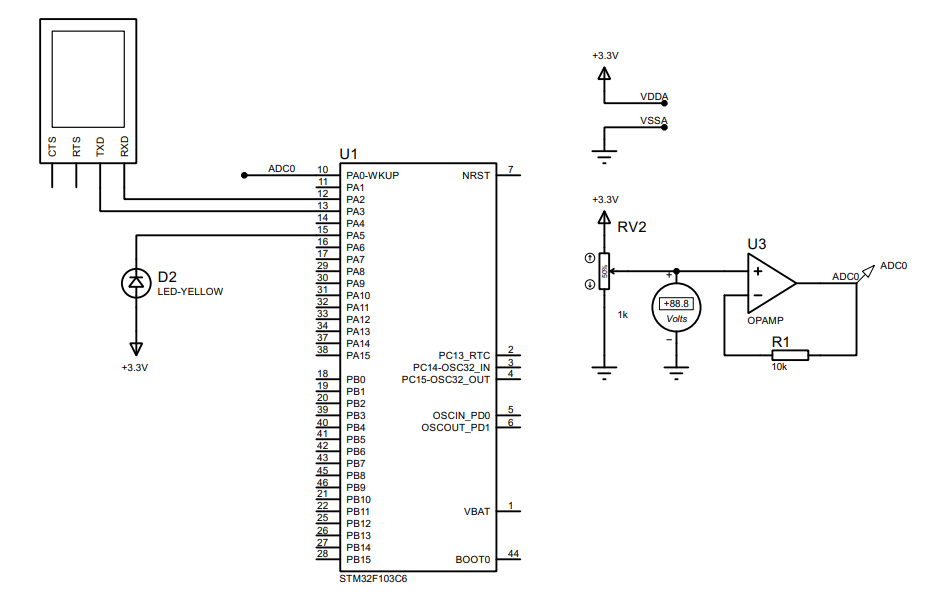
\includegraphics[width=5in]{source/picture/bai_6/Proteus_Simulation.PNG}
    \caption{\textit{Simulation circuit on Proteus}}
    \label{bai4_pic_button_schematic_0}
\end{figure}

Some new components are listed bellow:
\begin{itemize}
    \item Terminal: Right click, choose Place, Virtual Instrument, then select VIRTUAL TERMINAL.
    \item Variable resistor (RV2): Right click, choose Place, From Library, and search for the POT-HG device. The value of this device is set to the default 1k.
    \item Volt meter (for debug): Right click, choose Place, Virtual Instrument, the select DC VOLTMETER.
    \item OPAMP (U3): Right click, choose Place, From Library, and search for the OPAMP device.
\end{itemize}

The opamp is used to design a voltage follower circuit, which is one of the most popular applications for opamp. In this case, it is used to design an adc input signal, which is connected to pin PA0 of the MCU.\\

Double click on the virtual terminal and set its baudrate to 9600, 8 data bits, no parity and 1 stop bit, as follows:
\newpage
\begin{figure}[!htp]
    \centering
    \includegraphics[width=4in]{source/picture/bai_6/Proteus_Simulation2.PNG}
    \caption{\textit{Terminal configuration}}
    \label{bai4_pic_button_schematic_0}
\end{figure}

\section{Project configurations}
A new project is created with following configurations, concerning the UART for communications and ADC input for sensor reading. The pin PA5 should be an GPIO output, for LED blinky.
\subsection{UART Configuration}
From the ioc file, select \textbf{Connectivity}, and then select the \textbf{USART2}. The parameter settings for UART channel 2 (USART2) module are depicted as follows:

\begin{figure}[!htp]
    \centering
    \includegraphics[width=4.5in]{source/picture/bai_6/stm32_uart_1.PNG}
    \caption{\textit{UART configuration in STMCube}}
    \label{1}
\end{figure}

The UART channel in this lab is the Asynchronous mode, 9600 bits/s with no Parity and 1 stop bit. After the uart is configured, the pins PA2 (Tx) and PA3(Rx) are enabled. \\

Finally, the NVIC settings are checked to enable the UART interrupt, as follows:
\begin{figure}[!htp]
    \centering
    \includegraphics[width=3.5in]{source/picture/bai_6/stm32_uart_2.PNG}
    \caption{\textit{Enable UART interrupt}}
    \label{2}
\end{figure}

\subsection{ADC Input}
In order to read a voltage signal from a simulated sensor, this module is required. By selecting on \textbf{Analog}, then \textbf{ADC1}, following configurations are required:
\begin{figure}[!htp]
    \centering
    \includegraphics[width=4.5in]{source/picture/bai_6/stm32_adc_1.PNG}
    \caption{\textit{Enable UART interrupt}}
    \label{3}
\end{figure}

The ADC pin is configured to PA0 of the STM32, which is shown in the pinout view dialog. \\

Finally, the PA5 is configured as a GPIO output, connected to a blinky LED.

\section{UART loop-back communication}
This source is required to add in the main.c file, to verify the UART communication channel: sending back any character received from the terminal, which is well-known as the loop-back communication.

\begin{lstlisting}[caption= Implement the UART interrupt service routine]
/* USER CODE BEGIN 0 */
uint8_t temp = 0;

void HAL_UART_RxCpltCallback(UART_HandleTypeDef *huart){
	if(huart->Instance == USART2){
		HAL_UART_Transmit(&huart2, &temp, 1, 50);
		HAL_UART_Receive_IT(&huart2, &temp, 1);
	}
}
/* USER CODE END 0 */
\end{lstlisting}

When a character (or a byte) is received, this interrupt service routine is invoked. After the character is sent to the terminal, the interrupt is activated again. This source code should be placed in a user-defined section.\\

Finally, in the main function, the proposed source code is presented as follows:

\begin{lstlisting}[caption=Implement the main function]
int main(void)
{
  HAL_Init();
  SystemClock_Config();

  MX_GPIO_Init();
  MX_USART2_UART_Init();
  MX_ADC1_Init();

  HAL_UART_Receive_IT(&huart2, &temp, 1);

  while (1)
  {
	  HAL_GPIO_TogglePin(LED_RED_GPIO_Port, LED_RED_Pin);
	  HAL_Delay(500);
  }
  
}
\end{lstlisting}

\section{Sensor reading}
A simple source code to read adc value from PA0 is presented as follows:
\begin{lstlisting}[caption=ADC reading from AN0]
uint32_t ADC_value = 0;
while (1)
{
  HAL_GPIO_TogglePin(LED_RED_GPIO_Port, LED_RED_Pin);
  ADC_value =  HAL_ADC_GetValue(&hadc1);
HAL_UART_Transmit(&huart2, (void *)str, sprintf(str, "%d\n", ADC_value), 1000);
  HAL_Delay(500);
}
\end{lstlisting}

Every half of second, the ADC value is read and its value is sent to the console. It is worth noticing that the number ADC\_value is convert to ascii character by  using the sprintf function.\\

The default ADC in STM32 is 13 bits, meaning that 5V is converted to 4096 decimal value. If the input is 2.5V, ADC\_value is 2048.

\section{Project description}
In this lab, a simple communication protocol is implemented as follows:
\begin{itemize}
    \item From the console, user types \textbf{!RST\#} to ask for a sensory data.
    \item The STM32 response the ADC\_value, following a format \textbf{!ADC=1234\#}, where 1234 presents for the value of ADC\_value variable.
    \item The user ends the communication by sending \textbf{!OK\#}
\end{itemize}

The timeout for waiting the \textbf{!OK\#} at STM32 is 3 seconds. After this period, its packet is sent again. \textbf{The value is kept as the previous packet}.

\subsection{Command parser}
This module is used to received a command from the console. As the reception process is implement by an interrupt, the complexity is considered seriously. The proposed implementation is given as follows.\\

Firstly, the received character is added into a buffer, and a flag is set to indicate that there is a new data.

\begin{lstlisting}[caption= Add the received character into a buffer]
#define MAX_BUFFER_SIZE  30
uint8_t temp = 0;
uint8_t buffer[MAX_BUFFER_SIZE];
uint8_t index_buffer = 0;
uint8_t buffer_flag = 0;
void HAL_UART_RxCpltCallback(UART_HandleTypeDef *huart){
	if(huart->Instance == USART2){

		//HAL_UART_Transmit(&huart2, &temp, 1, 50);
		buffer[index_buffer++] = temp;
		if(index_buffer == 30) index_buffer = 0;

		buffer_flag = 1;
		HAL_UART_Receive_IT(&huart2, &temp, 1);
	}
}
\end{lstlisting}

A state machine to extract a command is implemented in the while(1) of the main function, as follows:
\begin{lstlisting}[caption= State machine to extract the command]
while (1){
    if(buffer_flag == 1){
        command_parser_fsm();
        buffer_flag = 0;
    }
}
\end{lstlisting}

The output of the command parser is to set \textbf{command\_flag} and \textbf{command\_data}. In this project, there are two commands, \textbf{RTS} and \textbf{OK}. The program skeleton is proposed as follows:
\begin{lstlisting}[caption= Program structure]
while (1){
    if(buffer_flag == 1){
        command_parser_fsm();
        buffer_flag = 0;
    }
    uart_communiation_fsm();
}
\end{lstlisting}

\subsection{Project implementation}
Students are proposed to implement 2 FSM in seperated modules. Students are asked to design the FSM before their implementations in STM32Cube.

%\chap{Real Time Operating System}

%\input{source/content/bai_8}
%\input{source/content/bai_9}
% \chap{Bài Tập Giữa Kì}
\section{Giới thiệu}
Trong yêu cầu của bài giữa kì, một đồng hồ analog với 12 bóng đèn hiển thị, trượng trưng cho 12 số trên đồng hồ. Bên cạnh đó, sẽ có 3 nút nhấn: nút MENU, INC và DEC (để tăng và giảm thông tin)\\

Để tiện lợi trong quá trình demo, đồng hồ sẽ có 12 giờ. Tuy nhiên, mỗi phút sẽ chỉ có 12 giây, và mỗi giờ cũng sẽ có 12 phút. 

Đồng hồ có 3 chế độ hoạt động như sau:
\begin{itemize}
    \item Mode 0: Đây là chế độ mặt định mỗi khi bật nguồn hoặc khởi động lại hệ thống. Thông tin giờ phút và giây sẽ được hiển thị trên màn hình. Tại một thời điểm, chỉ có tối đa 3 đèn được hiển thị. Nếu 2 thông tin (hoặc 3 thông tin) trùng nhau, thì chỉ 1 đèn sẽ được hiển thị. Khi đang ở chế độ này, thông tin về giờ phút giây sẽ được cập nhật theo đúng quy luật của đồng hồ.
    \item Mode 1: Khi đang ở Mode 0 và nhấn vào nút MENU, đồng hồ sẽ chuyển sang chế độ này để chỉnh giờ. \textbf{Thông tin về giờ phút giây sẽ ngừng cập nhật để người dùng chỉnh giờ}.  Chỉ một thông tin về giờ hiện tại sẽ được hiển thị. Khi nhấn nút INC và DEC, thông tin giờ sẽ được cộng thêm, hoặc trừ đi. Đồng thời, đèn hiển thị cũng sẽ được cập nhật trên mặt của đồng hồ. Lưu ý rằng, khi đang ở vị trí số 1, và nhấn nút trừ (DEC), thì thông tin giờ sẽ đếm vòng sang 12. Mỗi lần nhấn nút INC hoặc DEC, thông tin mới về giờ sẽ được lưu lại ngay lập tức.
    
    \item Mode 2: Khi đang ở Mode 1 và nhấn vào nút MENU, đồng hồ sẽ chuyển sang chế độ chỉnh phút. Chỉ một thông tin về phút hiện tại của được hiển thị trên màn hình. Việc chỉnh phút cũng được thực hiện tương tự như chỉnh giờ.
\end{itemize}

\textbf{Khi đang ở Mode 1 hoặc Mode 2, người dùng không tương tác vào bất cứ nút nào (MENU, INC hay DEC) trong vòng 5 giây, hệ thống tự động chuyển về Mode 0.}\\


Hệ thống sẽ được hiện thực trên phần mềm mô phỏng Proteus. Vi điều khiển STM32103C6 sẽ được sử dụng. Sinh viên không bắt buộc phải sử dụng ngắt timer. Nút nhấn chỉ tích cực mỗi khi nhấn xuống và \textbf{không kiểm tra trường hợp nhấn đè}. Ví dụ đang ở trạng thái chỉnh giờ, nút INC được nhấn xuống, giờ ngay lập tức sẽ được tăng lên 1 đơn vị. Tuy nhiên nếu cứ giữ đè, thì giờ vẫn không tăng. Nút nhấn được chống rung bằng cách đọc 2 lần liên tiếp giống nhau, mỗi lần cách nhau 10ms.


\section{Nộp bài}
Sinh viên hoàn thiện file report này, với các nội dung được yêu cầu bên dưới, file main.c
,tất cả các file .h và .c sinh viên hiện thực thêm sẽ được nén lại với MSSV và nộp lên hệ thống. \\

Sinh viên quay màn hình phần demo trên Proteus và tải lên Drive của mình (ở chế độ public). Link của video demo sẽ được trình bày ở phần cuối của Report.


\section{Report}
\subsection{Mô phỏng trên Proteus}
Thiết kế sơ đồ mạch điện trên Proteus, bao gồm 12 chân đèn LED và 3 nút nhấn. Để đơn giản, sinh viên có thể lược bỏ điện trở hạn dòng cho đèn LED.\\

Sinh viên chụp hình màn hình mô phỏng Proteus và dán vào phần report này.

\subsection{Thiết kế máy trạng thái}
Sinh viên thiết kế máy trạng thái cho hệ thống và trình bày ở phần này. Sinh viên được khuyến khích giải thích thêm cho máy trạng thái của mình để tiện lợi cho giảng viên khi đánh giá.

\subsection{Lập trình trên STM32Cube}
Trong trường hợp không sử dụng ngắt timer, cấu trúc chương trình sẽ như sau:

\begin{lstlisting}[caption=Cấu trúc chương trình trên main]
int main(void)
{
  HAL_Init();
  SystemClock_Config();

  MX_GPIO_Init();

  while (1){
    clock_fsm();
    timer_run();
    button_scan();
    HAL_Delay(10);
  }
}
\end{lstlisting}

Sinh viên sửa lại các hàm ở trên cho phù hợp với việc hiện thực của mình, chỉ giữ lại hàm HAL\_Delay(10) ở cuối cùng. Trong trường hợp sử dụng ngắt, sinh viên cấu hình là ngắt 10ms, không sử dụng HAL\_Delay và timer\_run, button\_scan  sẽ đặt trong hàm ngắt.\\

Từ phần này, sinh viên trình bày mã nguồn của từng module hiện thực, chẳng hạn như module timer (hàm chính sử dụng trong main là timer\_run), hàm đọc giá trị từ 3 nút nhấn (hàm chính sử dụng trong main là button\_scan). \\

Quan trọng nhất là mã nguồn cho phần xử lý máy trạng thái của đồng hồ. Một ví dụ cho việc trình bày mã nguồn mở, bao gồm file timer.h và timer.c

\subsection{Module Timer}
Đặc tả ngắn gọn về module này
\subsubsection{File timer.h}
\begin{lstlisting}[caption=Mã nguồn file .h]
#ifndef _TIMER_H_
#define _TIMER_H_

extern int timer0_flag;


void setTimer0(int duration);
void timer_run();

#endif
\end{lstlisting}
\subsubsection{File timer.c}
\begin{lstlisting}[caption=Mã nguồn file .c]
#include "timer.h"

int timer0_counter = 0;
int timer0_flag = 0;
int TIMER_CYCLE = 10;

void setTimer0(int duration){
	timer0_counter = duration / TIMER_CYCLE;
	timer0_flag = 0;
}

void timer_run(){
	if(timer0_counter > 0){
		timer0_counter --;
		if(timer0_counter <= 0) timer0_flag = 1;
	}
}
\end{lstlisting}


\section{Video demo}
Sinh viên cần quay 1 đoạn demo ngắn trên Proteus để minh họa việc chỉnh giờ, dừng 5 giây không chỉnh phút để thoát ra chế độ hoạt động bình thường. Sau đó nhấn vào MENU để chỉnh giờ, rồi nhấn tiếp MENU để chỉnh phút. Sau khi chỉnh phút xong (không tương tác trong 5s), hệ thống sẽ quay lại chế độ hoạt động bình thường.\\

Đường link cho video demo như sau:
\begin{center}
    \link{http://}
\end{center}

\end{document}

%%%%%%%%%%%%%%%%%%%%%%%%%%%%%%%%%%%%%%%%%%%%%%
%           GITHUB: phuongnam0907            %
%%%%%%%%%%%%%%%%%%%%%%%%%%%%%%%%%%%%%%%%%%%%%%